% !TEX program = lualatex
% !TEX encoding = UTF-8 unicode
\documentclass{book}
\usepackage{graphicx} % Required for inserting images
\usepackage{mdframed}


\usepackage{style}
\usepackage{circuitikz}
\usetikzlibrary{tikzmark}
\usepackage{tikz}
\usepackage{circuitikz}

% \newtcbox{\inlinecode}{on line,
%   box align=base,
%   colback=gray!20,
%   colframe=gray!50,
%   boxrule=0pt,
%   arc=1pt,
%   top=0.5pt,
%   bottom=0.5pt,
%   left=2pt,
%   right=2pt,
%   fontupper=\ttfamily\small
% }
% Define a custom style for x86-64 Assembly
\lstdefinelanguage[x64]{Assembler}%
  [x86masm]{Assembler}% base language
  {morekeywords=[1]{rax, rbx, rcx, rdx, rsi, rdi, rsp, rbp,
                    r8, r9, r10, r11, r12, r13, r14, r15,
                    eax, ebx, ecx, edx, esi, edi, esp, ebp},
   morekeywords=[2]{mov, push, pop, call, ret, jmp, je, jne, cmp, test,
                    add, sub, imul, idiv, xor, or, and, lea, inc, dec}}

% Custom style
\lstdefinestyle{asmstyle}{
    language=[x64]Assembler,
    basicstyle=\ttfamily\footnotesize,
    keywordstyle=[1]\color{blue},
    keywordstyle=[2]\color{purple}\bfseries,
    commentstyle=\color{gray}\itshape,
    morecomment=[l]{;},
    showstringspaces=false,
    columns=fullflexible,
    frame=single,
    captionpos=b
}

% Define a custom style for x86-64 Assembly
\lstdefinelanguage[x64]{Assembler}%
  [x86masm]{Assembler}% base language
  {morekeywords=[1]{rax, rbx, rcx, rdx, rsi, rdi, rsp, rbp,
                    r8, r9, r10, r11, r12, r13, r14, r15,
                    eax, ebx, ecx, edx, esi, edi, esp, ebp},
   morekeywords=[2]{mov, push, pop, call, ret, jmp, je, jne, cmp, test,
                    add, sub, imul, idiv, xor, or, and, lea, inc, dec}}

% Custom style
\lstdefinestyle{asmstyle}{
    language=[x64]Assembler,
    basicstyle=\ttfamily\footnotesize,
    keywordstyle=[1]\color{blue},
    keywordstyle=[2]\color{purple}\bfseries,
    commentstyle=\color{gray}\itshape,
    morecomment=[l]{;},
    showstringspaces=false,
    columns=fullflexible,
    frame=single,
    captionpos=b
}
\newtcbox{\inlinecode}{
    on line,
    boxsep=1pt,
    left=2pt,
    right=2pt,
    top=1pt,
    bottom=1pt,
    colback=gray!20,      % background (Markdown-like)
    colframe=gray!20,     % same color as background (no visible border)
    boxrule=0pt,
    arc=2pt,              % rounded corners
    box align=base,
    fontupper=\ttfamily
}
\let\oldtexttt\texttt
\renewcommand{\texttt}[1]{\inlinecode{#1}}

\lstdefinelanguage[RISC-V]{Assembler}
{
  alsoletter={.}, % allow dots in keywords
  alsodigit={0x}, % hex numbers are numbers too!
  morekeywords=[1]{ % instructions
    lb, lh, lw, lbu, lhu, li,
    sb, sh, sw,
    sll, slli, srl, srli, sra, srai,
    add, addi, sub, lui, auipc,
    xor, xori, or, ori, and, andi,
    slt, slti, sltu, sltiu,
    beq, bne, blt, bge, bltu, bgeu,
    j, jr, jal, jalr, ret,
    scall, break, nop
  },
  morekeywords=[2]{ % sections of our code and other directives
    .align, .ascii, .asciiz, .byte, .data, .double, .extern,
    .float, .globl, .half, .kdata, .ktext, .set, .space, .text, .word
  },
  morekeywords=[3]{ % registers
    zero, ra, sp, gp, tp, s0, fp,
    t0, t1, t2, t3, t4, t5, t6,
    s1, s2, s3, s4, s5, s6, s7, s8, s9, s10, s11,
    a0, a1, a2, a3, a4, a5, a6, a7,
    ft0, ft1, ft2, ft3, ft4, ft5, ft6, ft7,
    fs0, fs1, fs2, fs3, fs4, fs5, fs6, fs7, fs8, fs9, fs10, fs11,
    fa0, fa1, fa2, fa3, fa4, fa5, fa6, fa7
  },
  morecomment=[l]{;},   % mark ; as line comment start
  morecomment=[l]{\#},  % as well as # (even though it is unconventional)
  morestring=[b]",      % mark " as string start/end
  morestring=[b]'       % also mark ' as string start/end
}

\lstset{
  backgroundcolor=\color{gray!10},
  basicstyle=\ttfamily\small,
  keywordstyle=\color{blue},
  commentstyle=\color{green!60!black},
  stringstyle=\color{orange},
  showstringspaces=false,
  breaklines=true,
  frame=single,
}




\title{Computer Architecture \\ Prof. Paolo Ienne}
\author{Arthur Herbette}
\date{October 2025}

\begin{document}

\maketitle

\newpage
\tableofcontents
\newpage
\chapter{Introduction}
This document is the note I have written during and outside of the course, all the information here is directly taken from the course, slides, etc... However mistake can happen, if you see some mistake or see something that is not clear, feel free to ping an issue on the github, or email/telegram me.\\
\textbf{Disclaimer} in this course, when we say \textit{high-level language} we mean a language that is compiled/interpreted for instance: \texttt{c} is a high-level language here.
\subsection{Content of the course}
The course is divided into three parts:
\begin{itemize}
	\item \textbf{Part I: Processors and ISA}  \\ What is a processor? How can we design one? How do programs look like when they are executed? 
	\item \textbf{Part II: I/Os and Exceptions} \\ What is arounf a processor to make a full computer? How the processor exchanges information with the rest of the world? 
	\item \textbf{Part III: Memory Hierarchy} \\ Processors are fast and memory is slow -how can one combine the two? How can one protext the data users in memory
	\item \textbf{Parti IV: Instruction-Level Parallelism} \\ What makes a good processor? How real processors achieve ever increasing performances? 
	\item \textbf{Part V: Multiprocessors} \\ What are the basic challeng of connecting many processors together? What changes from a single processor system? 
	\item \textbf{Parti VI: Rudiments of Hardware Secrurity} \\ How can a hacker exploit what we have built in the previous parts to attack a system? How physics helps jeopardizing security?
\end{itemize}
\subsubsection{Literature}
The course will have two books for the literature which are the same as the one for fds :
\begin{enumerate}
    \item Digital Design: Principles and Practices John F. Wakerly 
    \item Computer organization and design: The hardware software interface David A. Patterson, John L. Hennessy
\end{enumerate}
\scalebox{0.4}{
\begin{circuitikz}
\tikzstyle{every node}=[font=\large]
\draw  (-3.25,30.5) rectangle (3,20.5);
\draw  (-1.25,29.75) rectangle  node {\LARGE Controller} (-1.25,29.75);
\draw  (1.75,29) -- (1.75,29) -- (2.25,29) -- (2.25,29) -- cycle;
\node [font=\normalsize] at (2,29.75) {sel\_imm};
\node [font=\normalsize] at (2,28.5) {branch\_op};
\node [font=\normalsize] at (1.75,28) {rf\_we};
\node [font=\normalsize] at (1.75,27.5) {sel\_addr};
\node [font=\normalsize] at (1.75,27) {sel\_b};
\node [font=\normalsize] at (2,26.5) {sel\_mem};
\node [font=\normalsize] at (1.75,26) {pc\_en};
\node [font=\normalsize] at (1.75,25.5) {pc\_sel\_pc\_base};
\node [font=\normalsize] at (1.5,24.75) {pc\_add\_imm};
\node [font=\normalsize] at (1.5,24.25) {pc\_sel\_alu};
\node [font=\normalsize] at (1.75,23.5) {sel\_pc};
\node [font=\normalsize] at (2,23) {we};
\node [font=\normalsize] at (2,22.5) {op\_alu};
\node [font=\normalsize] at (0.75,21) {imm};
\node [font=\normalsize] at (-1,21) {ir\_en};
\node [font=\normalsize] at (-2.25,24) {instruction};
\node [font=\normalsize] at (-2.5,25.5) {rst\_n};
\node [font=\normalsize] at (-2.5,27.25) {clk};
\draw (3,29.75) to[short] (4.25,29.75);


\draw (7.25,29.75) to[short] (7.5,29.75);
\draw (7.25,29.25) to[short] (7.5,29.25);
\draw (7.5,29.75) node[ieeestd and port, anchor=in 1, scale=0.89](port){} (port.out) to[short] (9.25,29.5);
\draw [ line width=0.7pt](3,29.75) to[short] (7.5,29.75);
\draw [ line width=0.7pt](6.75,29.25) to[short] (7.25,29.25);
\node [font=\normalsize] at (6,29.25) {alu\_res};
\draw [ line width=0.7pt](3,26) to[short] (10.75,26);
\draw [ line width=0.7pt](10.75,26) to[short] (10.75,29);
\draw [ line width=0.7pt](9.25,29.5) to[short] (10.75,29.5);
\draw (12.5,29.5) to[short] (12.75,29.5);
\draw (12.5,29) to[short] (12.75,29);
\draw (12.75,29.5) node[ieeestd or port, anchor=in 1, scale=0.89](port){} (port.out) to[short] (14.5,29.25);
\draw [ line width=0.7pt](10.75,29) to[short] (12.5,29);
\draw [ line width=0.7pt](10.75,29.5) to[short] (12.75,29.5);
\draw [ line width=0.7pt ] (16.75,31.75) rectangle (23.5,18.5);
\draw [ line width=0.7pt ] (20.5,24.75) rectangle  node {\Huge PC} (20.5,24.75);
\node [font=\normalsize] at (17.75,31) {clk};
\node [font=\normalsize] at (17.5,30.25) {rst\_n};
\node [font=\normalsize] at (17.75,27.5) {};
\node [font=\normalsize] at (18.25,26.75) {sel\_pb\_base};
\node [font=\normalsize] at (18.25,26) {add\_imm};
\node [font=\normalsize] at (18,24.75) {imm};
\node [font=\normalsize] at (17.75,24.25) {sel\_alu};
\node [font=\normalsize] at (17.75,23.5) {alu};
\node [font=\normalsize] at (17.25,29.5) {en};
\draw [ line width=0.7pt](14.5,29.25) to[short] (16.75,29.25);
\draw [ line width=0.7pt](16.75,30.25) to[short] (15.5,30.25);
\draw [ line width=0.7pt](16.75,31.25) to[short] (15.5,31.25);
\draw [ line width=0.7pt](3,25.75) to[short] (15,25.75);
\draw [ line width=0.7pt](16.75,26.75) to[short] (15,26.75);
\draw [ line width=0.7pt](15,26.75) to[short] (15,25.75);
\draw [ line width=0.7pt](16.75,26) to[short] (15.5,26);
\draw [ line width=0.7pt](3,25) to[short] (15.5,25);
\draw [ line width=0.7pt](15.5,26) to[short] (15.5,25);
\draw [ line width=0.7pt](3,24.25) to[short] (16.75,24.25);
\node [font=\normalsize] at (22.25,19.25) {addr};
\draw [ line width=0.7pt ] (3.25,12.75) rectangle (17.75,4.75);
\draw [ line width=0.7pt ] (-6.25,16) rectangle (-2.25,10.75);
\draw [ line width=0.7pt ] (-4.5,13.75) rectangle  node {\Huge IR} (-4.5,13.75);
\draw [ line width=0.7pt ] (10,8.75) rectangle  node {\Huge Register File} (10,8.75);
\node [font=\large] at (16.75,11.25) {a};
\node [font=\large] at (16.75,6.75) {b};
\draw [ line width=0.7pt](21.75,8.25) -- (22.25,8.25);
\draw [ line width=0.7pt](21.75,7.75) -- (22.25,7.75);
\draw [ line width=0.7pt] (22.25,8.75) -- (22.25,7.25) -- (23.25,7.75) -- (23.25, 8.25) -- (22.25,8.75);
\draw [ line width=0.7pt](23.25,8) -- (23.75,8);
\draw [ line width=0.7pt](22.75,9.25) -- (22.75,8.64);
\node [font=\large] at (22.75,8) {};
\draw [ line width=0.7pt](17.75,6.75) to[short] (21.75,6.75);
\draw [ line width=0.7pt](21.75,7.75) to[short] (21.75,6.75);
\draw [ line width=0.7pt](21.75,8.25) to[short] (19.75,8.25);
\draw [ line width=0.7pt](19.75,8.25) to[short] (19.75,15);
\draw [ line width=0.7pt](19.75,15) to[short] (6.25,15);
\draw [ line width=0.7pt](0.75,20.5) to[short] (0.75,15);
\draw [ line width=0.7pt](6.25,15) to[short] (0.75,15);
\draw [ line width=0.7pt](16.75,25) to[short] (16,25);
\draw [ line width=0.7pt](16,25) to[short] (16,15);
\draw [ line width=0.7pt](16.75,23.5) to[short] (15,23.5);
\node [font=\normalsize] at (14.25,23.75) {alu\_res};
\node [font=\normalsize] at (22,9.5) {sel\_b};
\draw [ line width=0.7pt ] (24.75,12.25) rectangle (28.5,6.5);
\draw [ line width=0.7pt ] (26.75,9.75) rectangle  node {\Huge ALU} (26.75,9.75);
\draw [ line width=0.7pt](23.75,8) to[short] (24.75,8);
\draw [ line width=0.7pt](17.75,11.25) to[short] (24.75,11.25);
\draw [ line width=0.7pt](26.75,12.25) to[short] (26.75,14.75);
\node [font=\large] at (26,14.75) {op\_alu};
\draw [ line width=0.7pt](28.5,9.5) to[short] (32.5,9.5);
\draw [ line width=0.7pt](32.5,9.75) -- (33,9.75);
\draw [ line width=0.7pt](32.5,10.25) -- (33,10.25);
\draw [ line width=0.7pt] (33,9.25) -- (33,10.75) -- (34,10.25) -- (34, 9.75) -- (33,9.25);
\draw [ line width=0.7pt](34,10) -- (34.5,10);
\draw [ line width=0.7pt](33.5,8.75) -- (33.5,9.64);
\node [font=\large] at (33.5,10) {};
\draw [ line width=0.7pt](32.5,10) to[short] (32.5,9.5);
\draw [ line width=0.7pt](32.5,10.25) to[short] (30.5,10.25);
\node [font=\large] at (30.5,10.75) {imm};
\node [font=\large] at (33.25,8.5) {sel\_imm};
\draw [ line width=0.7pt](38.25,9.5) -- (38.75,9.5);
\draw [ line width=0.7pt](38.25,10) -- (38.75,10);
\draw [ line width=0.7pt] (38.75,9) -- (38.75,10.5) -- (39.75,10) -- (39.75, 9.5) -- (38.75,9);
\draw [ line width=0.7pt](39.75,9.75) -- (40.25,9.75);
\draw [ line width=0.7pt](39.25,8.5) -- (39.25,9.39);
\node [font=\large] at (39.25,9.75) {};
\draw [ line width=0.7pt](34.5,10) to[short] (38.25,10);
\draw [ line width=0.7pt](22.25,18.5) to[short] (22.25,16);
\draw [ line width=0.7pt](22.25,16) to[short] (29,16);
\draw [ line width=0.7pt](29,16) to[short] (29,8.75);
\draw [ line width=0.7pt](29,8.75) to[short] (29,7.5);
\draw [ line width=0.7pt](29.25,7.5) to[short] (31.75,7.5);
\draw [ line width=0.7pt](29.5,7.5) to[short] (29,7.5);
\draw [ line width=0.7pt](32.25,7.25) -- (32.75,7.25);
\draw [ line width=0.7pt](32.25,7.75) -- (32.75,7.75);
\draw [ line width=0.7pt] (32.75,6.75) -- (32.75,8.25) -- (33.75,7.75) -- (33.75, 7.25) -- (32.75,6.75);
\draw [ line width=0.7pt](33.75,7.5) -- (34.25,7.5);
\draw [ line width=0.7pt](33.25,6.25) -- (33.25,7.14);
\node [font=\large] at (33.25,7.5) {};
\draw [ line width=0.7pt](31.75,7.75) to[short] (32.75,7.75);
\draw [ line width=0.7pt](31.75,7.5) to[short] (31.75,8);
\draw [ line width=0.7pt](34.25,7.5) to[short] (38,7.5);
\draw [ line width=0.7pt](38,7.5) to[short] (38,9.5);
\draw [ line width=0.7pt](38,9.5) to[short] (38.75,9.5);








\node [font=\large] at (33.25,6) {sel\_mem};



\draw [ line width=0.7pt](40,9.75) to[short] (43.75,9.75);
\draw [ line width=0.7pt](43.75,9.75) to[short] (43.75,4.5);
\draw [ line width=0.7pt](43.75,4.5) to[short] (23.5,4.5);
\draw [ line width=0.7pt](23.5,4.5) to[short] (19.75,4.5);
\draw [ line width=0.7pt](19.75,4.5) to[short] (19.75,2);
\draw [ line width=0.7pt](19.5,2) to[short] (1.75,2);
\draw (39,6.5) to[short] (39,6.75);
\draw (39.5,6.5) to[short] (39.5,6.75);
\draw (39,6.75) node[ieeestd or port, anchor=in 1, scale=0.89, rotate=90](port){} (port.out) to[short] (39.25,8.75);
\node [font=\large] at (39.75,6.25) {sel\_pc};
\draw [ line width=0.7pt](33.25,6.5) to[short] (39,6.5);
\draw [ line width=0.7pt](29.25,9.5) to[short] (29.25,17.25);
\draw [ line width=0.7pt](30.25,17.25) -- (30.75,17.25);
\draw [ line width=0.7pt](30.25,17.75) -- (30.75,17.75);
\draw [ line width=0.7pt] (30.75,16.75) -- (30.75,18.25) -- (31.75,17.75) -- (31.75, 17.25) -- (30.75,16.75);
\draw [ line width=0.7pt](31.75,17.5) -- (32.25,17.5);
\draw [ line width=0.7pt](31.25,16.25) -- (31.25,17.14);
\node [font=\large] at (31.25,17.5) {};
\draw [ line width=0.7pt](29.25,17.25) to[short] (30.25,17.25);
\draw [ line width=0.7pt](22.25,17.75) to[short] (30.5,17.75);
\node [font=\large] at (31.25,16) {sel\_addr};
\draw [ line width=0.7pt](32.25,17.5) to[short] (36.75,17.5);
\node [font=\large] at (4.25,11.75) {clk};
\node [font=\large] at (4,10.75) {aa};
\node [font=\large] at (4,9.75) {ab};
\node [font=\large] at (3.75,8.75) {aw};
\node [font=\large] at (4,7.75) {wren};
\node [font=\large] at (4,6.5) {wrdata};
\draw [ line width=0.7pt](1.75,2) to[short] (1.75,6.5);
\draw [ line width=0.7pt](1.75,6.5) to[short] (3.25,6.5);
\draw [ line width=0.7pt](1,7.75) to[short] (3.25,7.75);
\draw [ line width=0.7pt](0.5,8.75) to[short] (3.25,8.75);
\draw [ line width=0.7pt](-2.25,14.75) to[short] (2,14.75);
\draw [ line width=0.7pt](2,14.75) to[short] (2,10.75);
\draw [ line width=0.7pt](2,10.75) to[short] (3.25,10.75);
\draw [ line width=0.7pt](1,14.75) to[short] (1,9.75);
\draw [ line width=0.7pt](1,9.75) to[short] (3.25,9.75);
\draw [ line width=0.7pt](2.5,11.75) to[short] (3.25,11.75);
\draw [ line width=0.7pt](-0.75,14.75) to[short] (-0.75,10.5);
\draw [ line width=0.7pt](-1.5,14.75) to[short] (-1.5,18.25);
\draw [ line width=0.7pt](-1.5,18.25) to[short] (-4.75,18.25);
\draw [ line width=0.7pt](-4.75,18.25) to[short] (-4.75,23.75);
\draw [ line width=0.7pt](-4.75,23.75) to[short] (-3.25,23.75);
\draw [ line width=0.7pt](-9.25,27.75) to[short] (-3.25,27.75);
\draw [ line width=0.7pt](-9.75,25.5) to[short] (-3.25,25.5);
\draw [ line width=0.7pt](-8,15) to[short] (-6.25,15);
\draw [ line width=0.7pt](-7.75,12) to[short] (-6.25,12);
\end{circuitikz}
}
\chapter{Processors and instruction set architecture}
\section{Instruction set architecture}
The goal for the beggining of this course is to go from "high-level" perspective to the bottom of the iceberg. First let us look at a piece of code (\texttt{c}):

\begin{lstlisting}[language=c]
int data = 0x00123456;
int result = 0;
int mask = 1;
int count = 0;
int temp = 0;
int limit = 32;
do{
   temp = data & mask;
   result = result + temp;
   data = data >> 1;
   count = count + 1;
} while (count != limite);
\end{lstlisting}
Here we can see that we have variable with expressive names (that we can choose). each variable has a type, the computation we are doing \texttt{result + temp} looks like a mathematic formula, the control flow we are using is very intuitive.\\
In the case of those high-level language, we have an "unlimited" number of variables which supports any type.\\
If we wanted to convert this code into Assembly code we would have this:
\begin{lstlisting}[language={[RISC-V]Assembler}]
    li x1, 0x00123456
	li x2, 0 
	li x3, 1 
	li x4, 0 
	li x5, 0 
	li x6, 32
loop:
	and x5, x1, x3
	add x2, x2, x5 
	srli x1, x1, 1 
	addi x4, x4, 1 
	bne x4, x6, loop
\end{lstlisting}
As we can see we have a much more rigid format: we really have a sequence of numbered instructions that is executed line by line. For each instructions, we have an \textit{opcode}  that defines the effect of the instruction. Each \textit{variable} has a fixed name and we only have one form of control flow. The question to ask is why did we do that?\\ The answer of thie question lays is in the architecture of the processor:
\begin{center}
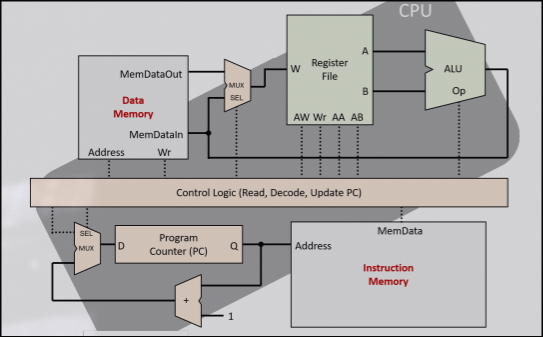
\includegraphics[scale=0.6]{screenshots/2025-10-11_1.png}
\end{center}
how it works: the processor fetch the instruction at the address of the program counter (PC) and launch it to the control logic
\begin{center}
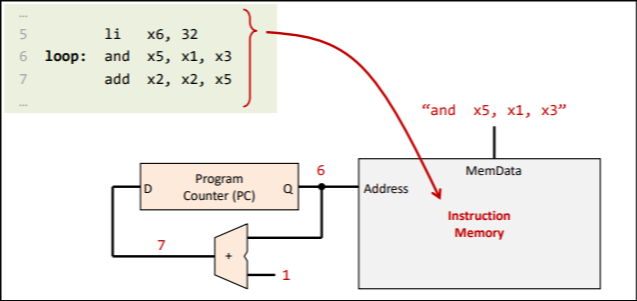
\includegraphics[scale=0.6]{screenshots/2025-10-11_2.png}
\end{center}
After that the instruction has been fetch, it is processed in the Control logic and then read/write etc... into the register file, and give the information (the opcode) to the ALU for it to know which operation to perform.
\begin{center}
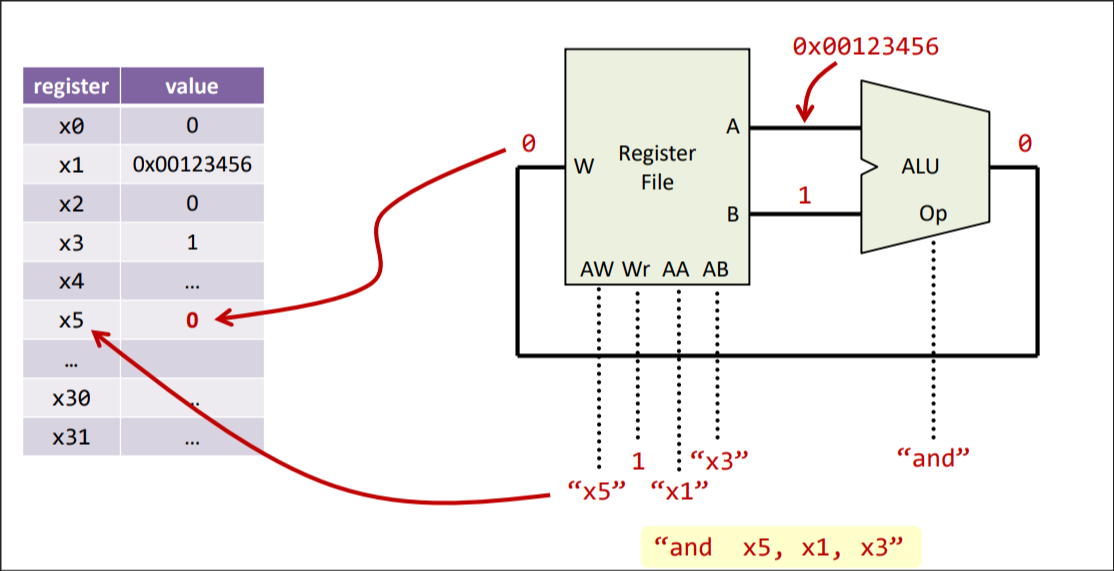
\includegraphics[scale=0.2]{screenshots/2025-10-11_3.png}
\end{center}
\subsubsection{The five classic components of a computer}
For an every day computer you need four other components other than the control components, you need to have a memory to store data (bigger than 32 word registers), you need to take input from the outside worlds (Internet, bluetooth, a keyboard, mouse ...) and also output something to the outside word.  On top of that, you need all of that to communicate $\implies$ you need a data path.
\begin{center}
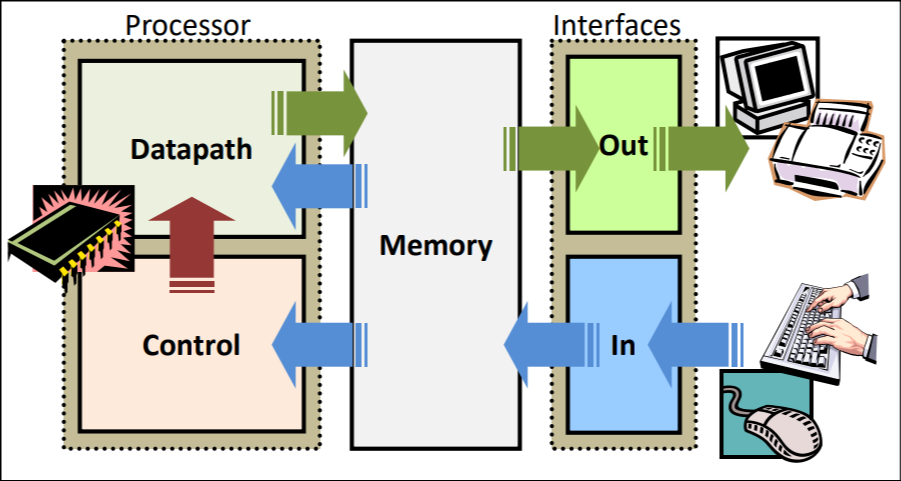
\includegraphics[scale=0.3]{screenshots/2025-10-11_4.png}
\end{center}
Okay, we have memory, we have input output and a place to compute everything, but what do we need to compute? Where is the program that is being executed? At the moment we have a place for the data but not for our program so how do we do it? \\ 
We store the program in the same memory than the one for the data. This is called a \textit{Unified Architecture} (On the other hand, an architecture that have two seperates memory, one for the instruction and one for the data is called a \textit{Harvard Architecture}). This is a \textbf{Key concept to computer science}, our instruction (therefore program) are represented as numbers (juste like data).
\begin{center}
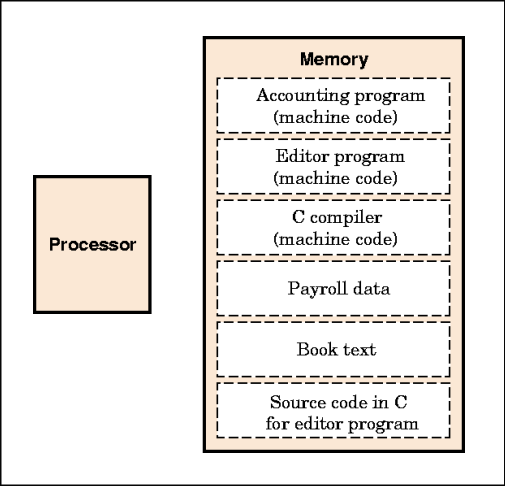
\includegraphics[scale=0.3]{screenshots/2025-10-11_5.png}
\end{center}
   Now a good question to have is: how to decode and encode those instructions and in the mean time, also what makes a good encoding? \\
A good encoding would be one that allows us two minimize the ressource in hardware and also is the fastest. This is where \texttt{RISC-V} comes in the play!! \texttt{RISC-V} is an instruction set architecture as like many others for instance x86, x64 for the most famous and used one.\\ 
The difference between assembly language and high-level language is in the "\textit{translation}", for the assembly language, we use an \important{assembler}, for a high-level language (a compiled one), we use a \important{compiler}:
\begin{itemize}
	\item Assembler can easily translate from code to binary code (this is what the instruction set tells us to do). All we need to do is the look up in the table and translate 
	\item A compiler on the other hand cannot look up in a table, it has to translate the code into Assembly code to be translated, but compiled the code into Assembly is a very hard thing to do, you have to find the best way or at least, try to find the best way to say the same thing but in assembly.
\end{itemize}




	\section{Instruction set architecture: Branches, Function and stack}
	The main goal that ISA does is to put a \textbf{Contract} between the hardware and the software: If you are an hardware person, all you care about is the make your processor the fastest on the ISA. If you are a software person, you don't need to worry about the hardware behind anything, you only care about the software that you are building. This ISA gives a level of abstraction which makes it easier to develop better software/hardware.
	\begin{center}
	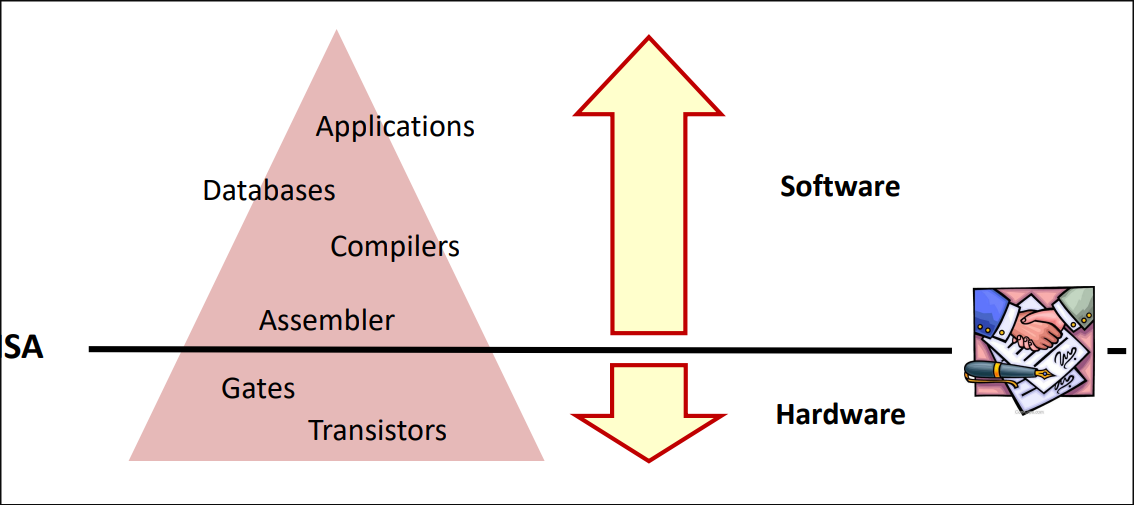
\includegraphics[scale=0.3]{screenshots/2025-10-11_6.png}
	\end{center}
	As we have seen in cs-173, arithmetic and logic operation are quite easy to understand and use in RISC-V. But here are some facts to know about them:
	\begin{itemize}
		\item Immediate constant takes at maximum 12 bits. The reason behind this is that the immediate part of the instruction is directly stored in the instruction, this means that there are 12 bits of the instruction that are reserved for the immediate part. Imagine having for instance a 30 bits immediate, then you would only have 2 bits for: the opcode, result register, input register ... 
		\item A way to go around this is to use the \texttt{.equ, num} and then to use \texttt{lui} directly on \texttt{num}. (this is possible because the assembler will directly translate the one line instruction into a three lines instruction). 
		\item Register \texttt{x0}, this register is \textbf{always} zero (by definition), you can write anything to this resgister, the value in it will always be zero. This can be useful  in a lot of case, it happens quite often that we need a zero in a instruction and the only way to do so would have been to \texttt{li} a register to 0 and then calling the instruction. Therefore, the \texttt{x0} register allows us to save instructions
	\end{itemize}

	\subsubsection{An if-then-else}
	To be able to do an if and else cause will need some branches, for instance if we wanted to translate the code:
	\begin{lstlisting}[language=c]
	if (x5 == 72) {
	   x6 = x6 + 1
	} else {
	   x6 = x6 - 1
	}
	...
	\end{lstlisting}
	Into RISC-V: it would look like this:
	\begin{lstlisting}[language={[RISC-V]Assembler}]
	.text 
		li x7, 72
		beq x5, x7, then_clause
	else_clause:
		addi x6, x6, -1 
		j end_if
	then_clause:
		addi x6, x6, 1 
	end_if:
		...
	\end{lstlisting}
	As you can see jump and branch are really similar however, there is a universal distinction between them:
	\begin{itemize}
		\item Jumps $\to $ \important{unconditional} control transfer instructions
		\item Branch $\to $ \important{conditional} control transfer instructions
	\end{itemize}
	However this is not the case for every assembly languages, for instance in x86, everything is defined as a jump.
	\subsubsection{A Do-while loop}
	\begin{center}
		A do while loop in c
	\end{center}

	\begin{lstlisting}[language=c]
	do {
	   x5 = x5 >> 1 
	   x6 = x6 + 1 
	} while (x5 != 0);
	...
	\end{lstlisting}

	\begin{center}
		A do while loop in risc-v
	\end{center}
	\begin{lstlisting}[language={[RISC-V]Assembler}]
	.text
	loop:
		srli x5, x5, 1 
		addi x6, x6, 1 
		bnez x5, loop 
	...
	\end{lstlisting}
	\subsection{Functios}
	In our high-level code, we usually use function to organized our code (Scala...) (those function can also be called methods, procedure dependeing of the context).\\ 
	What we would like is also to have function in assembly so that we don't have to write the same code always. What a function would look like is:
	\begin{enumerate}
		\item Place arguments where the called function can access them 
		\item jump to the function 
		\item Acquire storage resources the function needs 
		\item Perform the desired task of the function 
		\item Communicate the result value back to the calling program 
		\item realease any local storage resources 
		\item Return control to the calling program
	\end{enumerate}
	That sound pretty hard to do so let's do it step by step. First, the second and seven steps (I know).\\
	What we need is to jump to the function and the return. This is fairly easy to do, all we need is to call the jump instruction. For instance, let's call the function two times. This  would looks like this
	\begin{lstlisting}[language={[RISC-V]Assembler}]
	sqrt:
		...
		j back
	\end{lstlisting}
	And the main would look like this:
	\begin{lstlisting}[language={[RISC-V]Assembler}]
	main: 
		...
		j sqrt 
	back:
		...
		j sqrt 
	back2:
		...
	\end{lstlisting}
	However, isn't there an issue? what would happen if we tried to run this code?\\
	The answer is that this would lead to an infinite loop. the \texttt{sqrt} function doesn't know about the fact that there are more than one back.
	The solution to this problem is to:\\
	when you called the function, you store the current PC $+ 4$  (to go to  the next line) to a register (for instance \texttt{x1}). You then, call the function, do the computation there \textbf{and then} you rejump to the address store in the register \texttt{x1}.

	\begin{parag}{Jump and link}
		


	There is instruction that allows us to do this, those instruction are called jamp and link \texttt{jal}, and the other one is called jump to the address specified in a register \texttt{jr}, however we said before that we only use \texttt{x1} for the return address so why don't we make an instruction that directly jump to this address: \texttt{ret} (which stands for return I think).\\
	However what we have to be careful with here is that the \texttt{x1} register is not preserved accorss the call (this is not something that is known for now but let me explain it shortly). What we will want to do is the call function inside function (have call inside call inside call etc ...) however every time we make a call to a function, the x1 register will be overwritten: every time you jump and link, you store in the return address register the pc $+ 4$. However this is not currently a problem, we will solve it later.
\paragraph{Acquire storage ressource the function needs}
There is a lot of way to do this. The first way to do so is to juste allocate like 10 registers to the current function and the rest to the function that is called. for instance
if we have this code:
\begin{lstlisting}[language={[RISC-V]Assembler}]
main:
	...
	jal sqrt 
	... 

	... 
	jal sqrt
	...
ret 

sqrt: 
	...

	add x5, x7, x8 
	jal round 
	sub x6, x6, x5 
	...
	ret

round:
	...
	addi x10, x11, 3 
	...

	ret
\end{lstlisting}
You see that the round procedure only use the register \texttt{x10} to \texttt{x15}. and that sqrt the one from 2 to 9. We can clearly see that this is not scalable, so we need another solution.
\end{parag}
\subsection{The stack}
The \important{stack} is the solution!! Fisrt what is the stack:\\
\begin{definition}
$ $\\
\begin{itemize}
    \item The stack is a empty region in the memory 
    \item We use the register \texttt{x2} (also called \texttt{sp}) to store the address of the end of the used region
    \item If we are using all variables and we still want to make a call to a function, we need to store in the stack our variable before calling the function and then restore our variable from the stack.
\end{itemize}
\end{definition}
The complexity of this is to understand the order of what is needed to be stored or not. For instance if you have a function that is being called from above. We have to be sure that we don't overwrite the values from the function that is above. to do so, we store the value in the stack and restore them afterward. (only the register that we are changing). to do so we have to dynamically allocate more space in the stack.\\ 
Here is an example:
\begin{lstlisting}[language={[RISC-V]Assembler}]
	...
	addi sp, sp, -8 
	sw x8, 0(sp)
	sw x9, 4(sp)
	...
	#we have here free use of x8 and x9
	...
	lw x9, 4(sp)
	lw x8, 0(sp)
	addi sp, sp, 8
\end{lstlisting}
However, do we need to store all the register? how do we return something, how do we pass arguements to a function. To do so we agree to use some register as arguement, return register, other for return address, stack pointer, temporaries, saved... I strongly advise to go read the RV32i Reference Card.\\
So what do we still need? we are currently able to jump to function, return from the function, acquire storage resources, perform the desired stack of the function, All we need is the arguement and return values.
To do so is very simple, as I said before we can:
\begin{itemize}
    \item Use some particular registers, both for the \important{arguments} and for the return \important{result}.
    \item We can do it ad-hoc ...
		\begin{itemize}
		    \item \texttt{sqrt} gets the arguement in \texttt{x5} and returns the result in \texttt{x6}
		\end{itemize}
	\item Or we can have some convention
		\begin{itemize}
		    \item All function pass arguements in register \texttt{x10} to \texttt{x17} and return the result in \texttt{x10}
		\end{itemize}
		\item Can this be insufficient? \important{More arguments} than allocated registers? What if we have 10 arguements
\end{itemize}

\paragraph{Option 2}
If we don't have enough registers, we can just put them in the task right? we know that the stack is unlimited (in theory), all we would need is to do more work (allocate space, storing, loading etc ...)\\
To do so we can use another register: \texttt{fp} or \texttt{x8} in risc-v which point to the same location as sp on entry. \\
This make the code more readable because:
\begin{itemize}
	\item \texttt{sp} changes inside the function and so do relative offsets 
	\item offests with respect to the \texttt{fp} are \important{fixed}
\end{itemize}
The use of the fp register is \important{optional} and even varies among users and compilers. (I personnaly didn't use it during lab 1, I only used the registers that are reserved).\\
\begin{center}
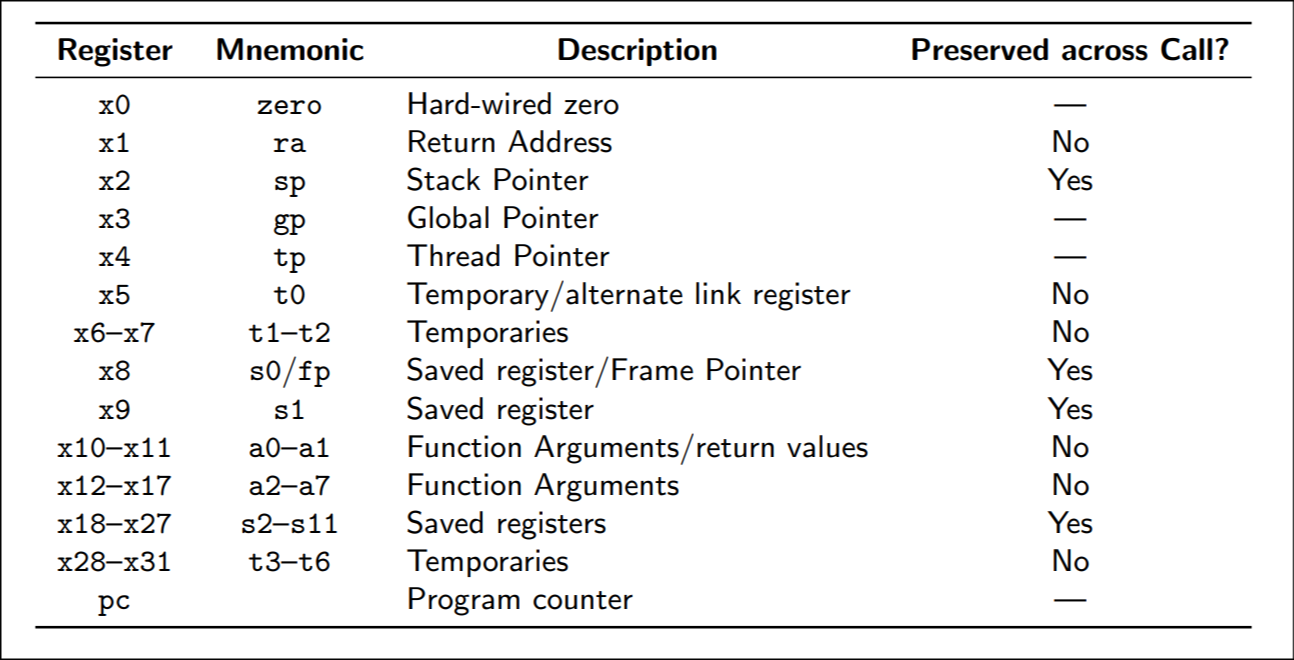
\includegraphics[scale=0.3]{screenshots/2025-10-11_7.png}
\end{center}


















\section{Memory and Addressing Modes}
\subsection{Memory}
Memory is an incredibly important component of a computing system:
\begin{itemize}
    \item We store our \important{programs} in it 
    \item We store our \important{data} in it 
	\item It is often through memory that we will \important{receive data and send out data}
\end{itemize}
	Memory is a reccurent ropic in this course, we have already seen it with the stack however the type of the memory is also an important topic:
	\begin{itemize}
		\item Memory can be \important{very slow} $\implies $ Caches 
		\item Memory is \textit{finite} (relatively small) $\implies $ Virtual memory 
		\item Memory can make an \important{ISA too complex} $\implies $ pipelining
	\end{itemize}
	\paragraph{Types of memory}
	There is a lot of different technologies for memory:
	\begin{itemize}
		\item SRAM, DRAM, EPROM, Flash, etc.
\end{itemize}
Each of those has a variations in \important{capabilities} therefore also in how we use them, memory change by:
\begin{itemize}
	\item Capacity, density 
	\item Speed 
	\item Writable, permanent, reprogrammable
\end{itemize}
\begin{center}
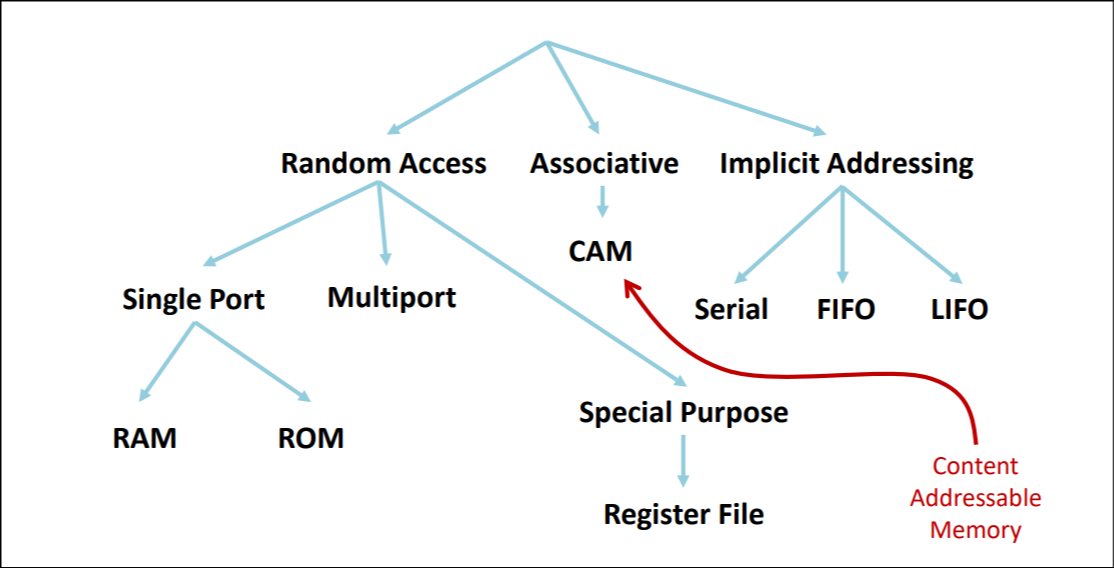
\includegraphics[scale=0.4]{screenshots/2025-10-11_8.png}
\end{center}
We have here all the type of memory that can be used, What we use when we program are Random access memory, this means that the memory can be accessed with an address. In the tree of random access memory we have:
\begin{center}
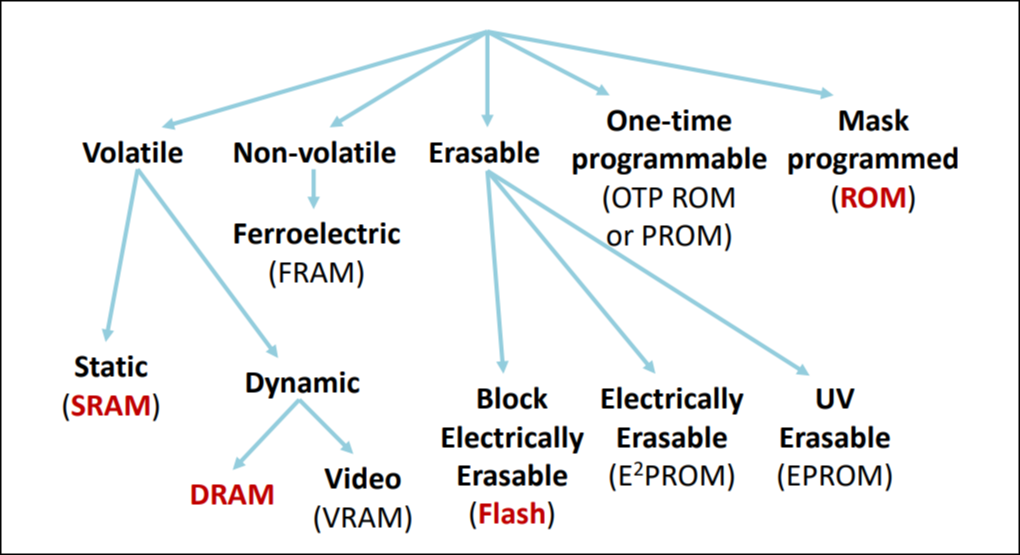
\includegraphics[scale=0.4]{screenshots/2025-10-11_9.png}
\end{center}
The basic structure behind those memory are DFF, (D flip flop). which are stacked one on another in a $n$ times 4 grid. Each flip flop looks like this:
\paragraph{SRAM}
SRAM stands for \important{static random access memory}. It sores data with flips flops which makes it faster than DRAM (which we will see later) but more expensive. We use it for CPU caches and for the register file
\begin{center}
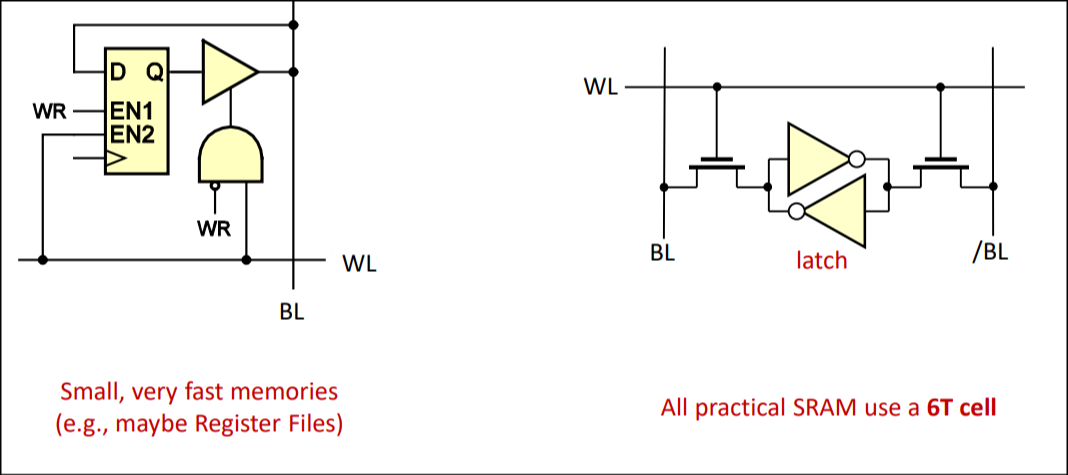
\includegraphics[scale=0.3]{screenshots/2025-10-11_10.png}
\end{center}
So here we have to make a difference between the boolean system and the electrical components. The circuit on the left is a desastre in term of electrical components it has approximatevely 20 transistors which makes it \important{slower} \textbf{and} \important{costlier}. The real way to do SRAM is with the right circuit. However this looks bad, normally it is forbidden to have a closed loop in a circuit! We are forbidden to have a loop in our circuit without a flip flop in it, you cannot have a loop inside a combinational circuit. So this is a big special thing for us however, this "works", it is compatible there is no issue in the circuit. The issue we have is that:\\
Imagine putting a one on the left or right part of the circuit $\implies$ the value cannot be changed, it is stucked there for ever. This looks really good because one \textbf{NOT} gate costs us only two transistors so the memory (loop) costs us only 4 transistors. But we still need to write and read from the memory, to do so we had the two transistors (see on the image) which also us to let the memory live on its own (when the transistors are open) \textbf{or} to be connected to the world. \\
If I want to see what is on the memory I put one in the word line (WL) and I will get the value on the bit line.\\
The question now is how to write? As said earlier, now we have a signal that is stored in there but it is stored for infinity.\\
The only way to write is to "\textit{shout louder than the current signal}".  Imagine we currently have a 1 as the output of the latch and I want to put a 0. If I shout 0 louder than the 1 while connected, it will have a short circuit... and this is bad. \textbf{However} what is going on in fact is the upper not gate will have two inputs, a \textbf{loud} 0 and a quiet 1, the not fate will then take the loudest one thus 0.\\
And now it will take a really short time to the latch to adapt itself to the new value, the short circuit here take the times two the 0 to go trhough two not gates. and then it agrees.\\

On the other hand we have DRAM:
\paragraph{DRAM}
\begin{itemize}
    \item  Dynamic RAMs are the densest (and thus cheapest) form of random access semiconductor memory 
    \item DRAMs store \important{information as charge in small capacitors} part of the memory cell 
    \item First parented in 1968 by Robert Dennard, scaled amazingly over decades and was somehow an important ingredient of the progress of computing systems.
    \item charges \important{leaks off} the capacitors due to parasitic resistance $\implies $ every DRAM cell needs a \important{periodic refresh} (e.g. every \~60ms) lest it forgets information.
\end{itemize}
So imagine, if we don't go in each cell every 60ms then we lose the information, but we have other things to do? So how do we do it? - we have someone else refresh them for us. The memory controller is reponsible for refreshing the contents of the DRAM instead of the CPU.
\begin{center}
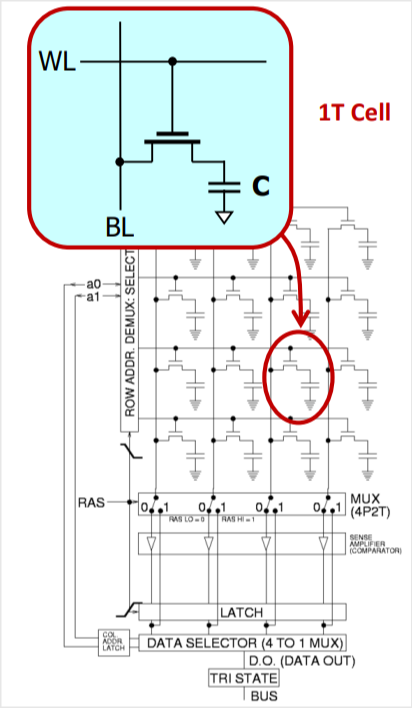
\includegraphics[scale=0.3]{screenshots/2025-10-12.png}
\end{center}
The goal after this is to access those memory celle based on the address we input. The \textit{ideal} way to do so, would be to have one \textbf{big} decoder that treats the adress and directly output the information in the memory celle like this:
\begin{center}
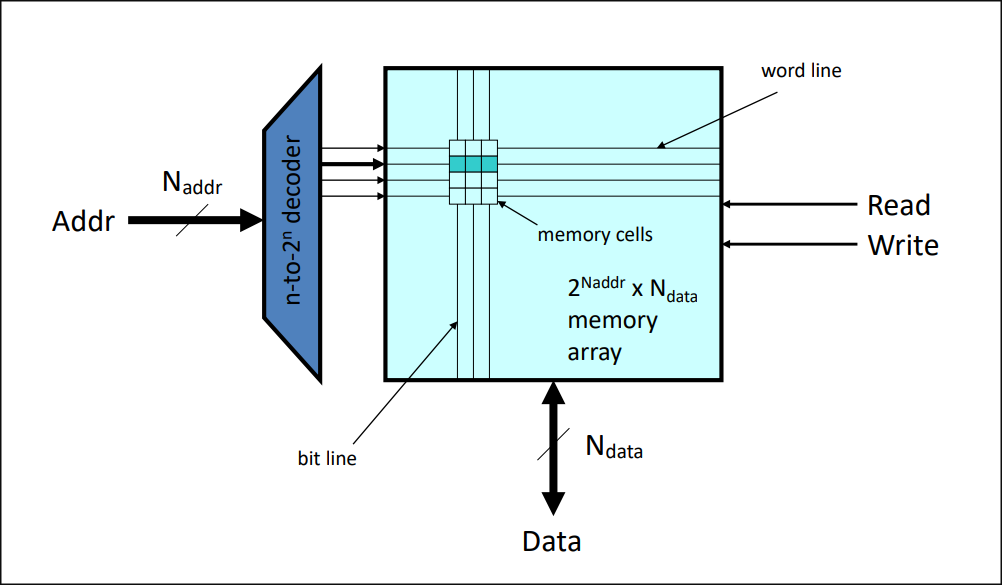
\includegraphics[scale=0.2]{screenshots/2025-10-12_1.png}
\end{center}
However life is not always that easy, and there is a lot of way to get the memory celle based on the address, here are some example:
\begin{center}
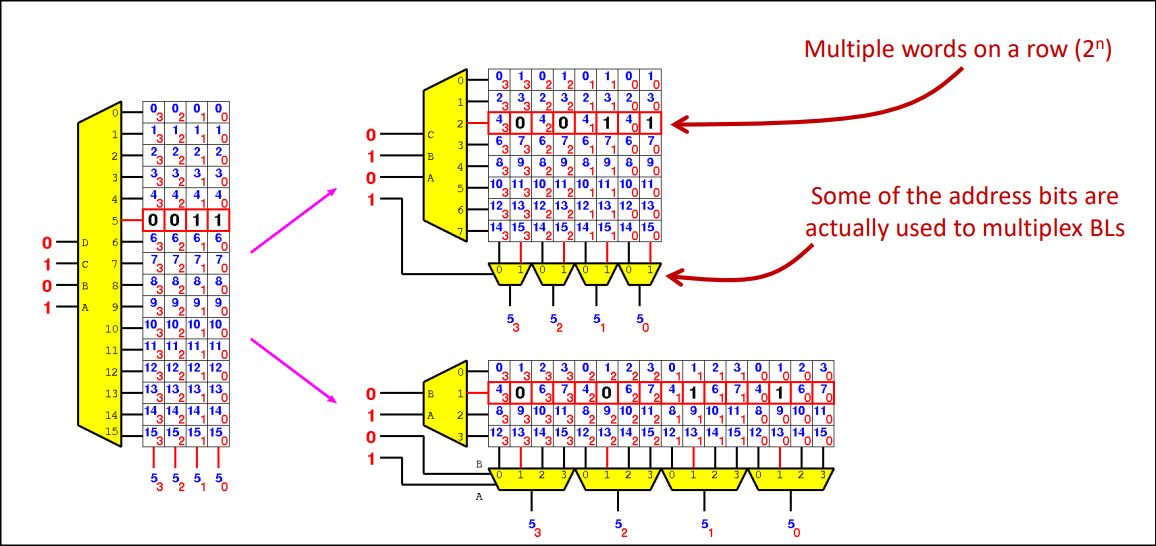
\includegraphics[scale=0.4]{screenshots/2025-10-12_2.png}
\end{center}
Here we have 3 ways to do so:
\begin{itemize}
    \item On the left, We have the same way as the \textit{ideal} decoder with one byte per row 
    \item However we can also split up into a grid with more than one \textbf{big} multiplexer. This implies that there will be multiple word by row and that the bytes are not necesserly ordered.
\end{itemize}
The best physical way to create a Random access memory is in a square to minimize parasitic capacitance of BL (bit line) and WL (word line). We want to having it into the most squared possible form because:
\begin{itemize}
	\item When a word line is activated (row), the bit line carries the data (bit) stored in the selected memory cell to the output circuitry (like a multiplexer or sense amplifier).
	\item Activating a word line selects all the bits (across bit lines) in that row — this is your selected "word."
\end{itemize}
Therefore by having the smallest length, we get shorter lines $\implies $ lower parasitic capacitance $\implies$ faster access, lower power, and more reliable operation.
\begin{center}
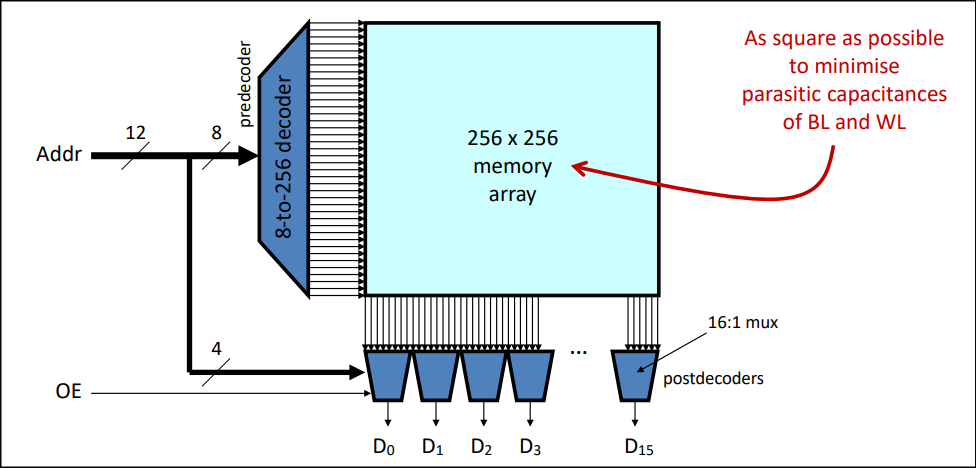
\includegraphics[scale=0.3]{screenshots/2025-10-12_3.png}
\end{center}

\begin{framedremark}

Every time we are looking for a memory cell, we need to charge all row and then all column, the goal here is to minimize the number $x =r + c$ by a fixed area $A$ (where $A$ is the number of cell):\\
We have that
\begin{align*} A = rc \\
				\frac{A}{c} = r
\end{align*}
Which implies that $x = \frac{A}{c} + c$, we are minimizing  ($x' = 0$) this:
\begin{align*} 
	x' = -\frac{A}{c^2} + 1 \\
	\frac{A}{c^2} = 1 \\
	c^2 =  A \implies c = \sqrt{A}
\end{align*}
And because we know that $A =  rc \implies r =  c =  \sqrt{A}$ which is a square.

\end{framedremark}
\paragraph{Static RAM typical interface}
This is the typical synchronous SRAM that we have already seen before:
\begin{center}
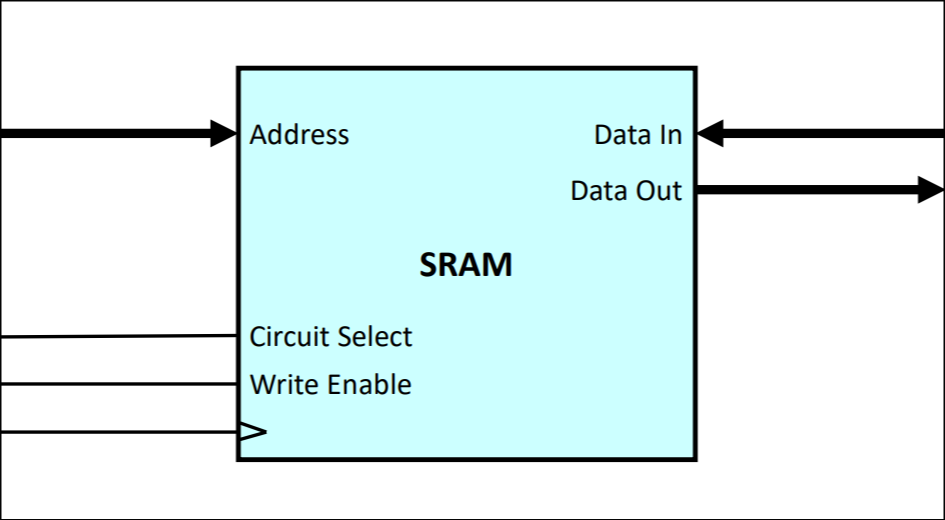
\includegraphics[scale=0.2]{screenshots/2025-10-12_4.png}
\end{center}
However we don't always has to be synchronous, we can also be asynchronous for a Read cycle which works like this:
\begin{parag}{Asynchronous read cycle}
    

\begin{itemize}
    \item Enable the memory $\to$ assert the address $\to $ wait for the data 
		\begin{itemize}
		    \item Data out is available after a combinational delay $T_{acc} = $ Access Time 
		\end{itemize}
		\item Maximum frequency is limited by the minimum $T_{cyc}$ (time for a cycle, time for us to be able to change the address)
\end{itemize}

\begin{center}
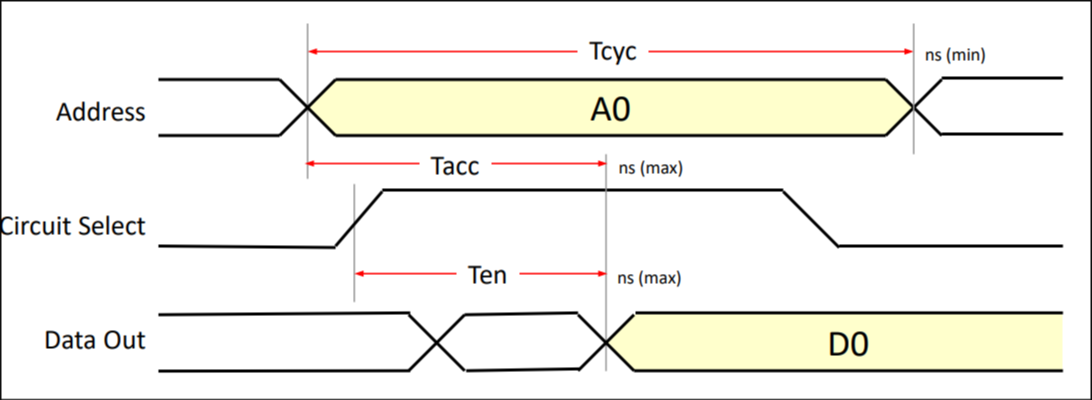
\includegraphics[scale=0.25]{screenshots/2025-10-12_6.png}
\end{center}

\end{parag}
\begin{parag}{synchronous SRAM Read cycle}
    

Here this is the other way around, we always wait a rising edge of the clock to do anything. Everything here is working like a flip flop:
\begin{itemize}
    \item Everything is relative to the clock signal
    \item Latency is the number of cycles between the address asserted and data available
		\begin{itemize}
			\item Often one as in this diagram but in some cases (large memories) more
		\end{itemize}
\end{itemize}


\begin{center}
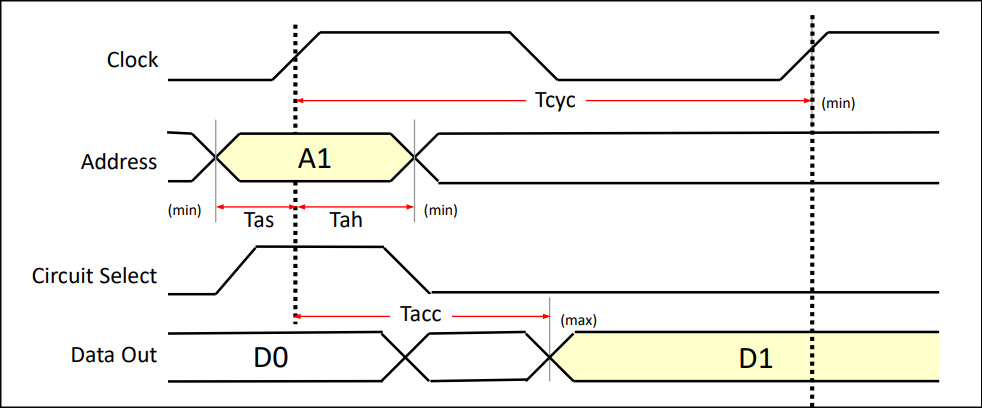
\includegraphics[scale=0.25]{screenshots/2025-10-12_7.png}
\end{center}
\end{parag}
\subsubsection{Load and store instrucitons}
Now that we have seen how it works, we want to see how to implement a load from the memory into the register file. For instance the following intrsuction:
\begin{lstlisting}[language={[RISC-V]Assembler}]
lw x5, (123456)
\end{lstlisting}
This is not a RISC-V instruction but bear with us. (I am not sure that's a saying...)


\begin{center}
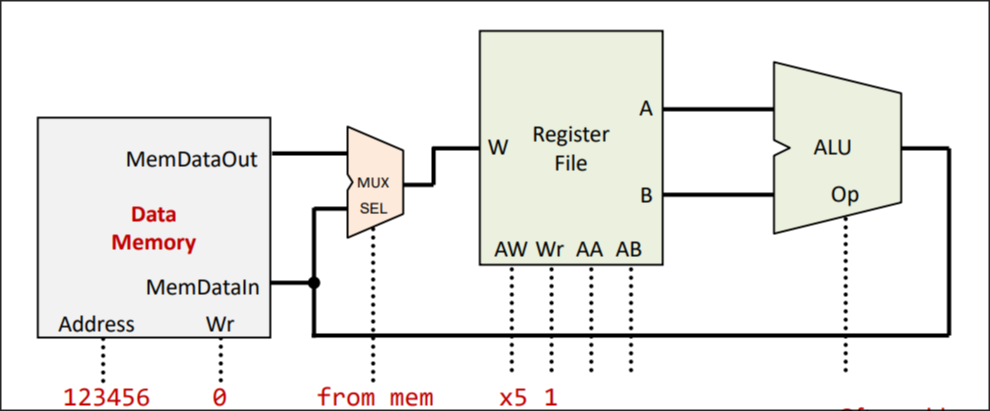
\includegraphics[scale=0.3]{screenshots/2025-10-12_8.png}
\end{center}
What we have changed here is the left part now instead of having a loop like $\text{ALU} \to \text{Register file} \to \text{ALU}$ we break it at the first "$\to$" and add a multiplexer there to be able to interact with the memory. \\

For the store instruction, instead of using the \texttt{MemDataOut} path, we use the \texttt{MemDataIn}.\\
The main diffrence is this:
\begin{center}
    


\begin{tikzpicture}[
    block/.style = {draw, minimum width=2.4cm, minimum height=1cm, align=center},
    arrow/.style = {thick, -{Latex}},
    node distance=1.8cm and 1.8cm
]

%% LOAD PATH

\node[block] (regfileL) {Register File\\(base)};
\node[block, right=of regfileL] (aluL) {ALU\\(base + offset)};
\node[block, right=of aluL] (memL) {Memory};
\node[block, right=of memL] (outregL) {Register File\\(destination)};

\draw[arrow] (regfileL) -- (aluL);
\draw[arrow] (aluL) -- (memL);
\draw[arrow] (memL) -- node[above]{\scriptsize{MemDataOut}} (outregL);

\node[above=0.5cm of aluL] {Load Instruction};

%% STORE PATH

\node[block, below=2.5cm of regfileL] (regfileS1) {Register File\\(base)};
\node[block, right=of regfileS1] (aluS) {ALU\\(base + offset)};
\node[block, right=of aluS] (memS) {Memory};

\node[block, below=1.5cm of aluS] (regfileS2) {Register File\\(value)};
\draw[arrow] (regfileS1) -- (aluS);
\draw[arrow] (aluS) -- (memS);
\draw[arrow] (regfileS2) -- node[right]{MemDataIn} (memS);

\node[above=0.5cm of aluS] {Store Instruction};

\end{tikzpicture}
\end{center}
\begin{framedremark}
	I had some trouble understand how does the value just pop, but if I understand it right, the register value is stored from the register file into \texttt{B} here. We use the \texttt{A} port as a address base. This is how it works:
\begin{enumerate}
    \item IF, Fetch instruction ( \texttt{sw x2, 8(x1)})
    \item ID, Read \texttt{x1} and \texttt{x2} from register file 
    \item EX, ALU compute \texttt{x1 + 8} (address) 
    \item MEM, Store \texttt{x2} to memory at computed address 
    \item WB, Nothing (no register to write for store)
\end{enumerate}
\end{framedremark}

\paragraph{Why RISC-V instructions are so simple?}%
\label{par:Why RISC-V instructions are so simple?}

\begin{framedremark}
Here are some example of some instruction that would look correct in RISC-V but is not (for addition):
\begin{itemize}
    \item Based or Indexed
		\begin{lstlisting}[language={[RISC-V]Assembler}]
	add x0, x1, i5(x2)		#x0 = x1 + mem[x2 + i5]
		\end{lstlisting}
	\item Auto-increment or -decrement
		\begin{lstlisting}[language={[RISC-V]Assembler}]
	add x0, x1, (x2+) 		#x0 = x1 + mem[x2]
		\end{lstlisting}
	\item PC-relative
		\begin{lstlisting}[language={[RISC-V]Assembler}]
	add x0, x1, 123(pc)		#x0 = x1 + mem[pc + 123]
		\end{lstlisting}
\end{itemize}
However those instruciton \important{does not exist} in RISC-V.\\
RISC-V is designed to have  two world: one for accessing memory, and one for the logic/arithmetic etc. We cannot mix them together.\\
However in x86/x64 we can do this:
\begin{lstlisting}[language={[x64]Assembler}]
	ADD DWORD PTR [EBX + ESI*4 + 16], EAX
\end{lstlisting}
This means:
\begin{itemize}
    \item The \texttt{DWORD} means double word which means that we are working on 64 bits number.
	\item The \texttt{ADD} that has only two operand, the reason why, is that the goal of x86 in 1979 was to be the most compact possible, at that time the memory was limited and to be able to write program you had to be careful of the size of the program that you are writing. So they added the constraints that the output of the instruction is stored in the first operand. \\ this means we take something in the memory at \texttt{[EBX + ESI*4 + 16]}, add it with \texttt{EAX} and then store it in \texttt{[EBX + ESI*4 + 16]}. 
\end{itemize}
	 this feels pretty slow and pretty confusing, just try to map this into the CPU we created before, this would look like this:
		\begin{center}
		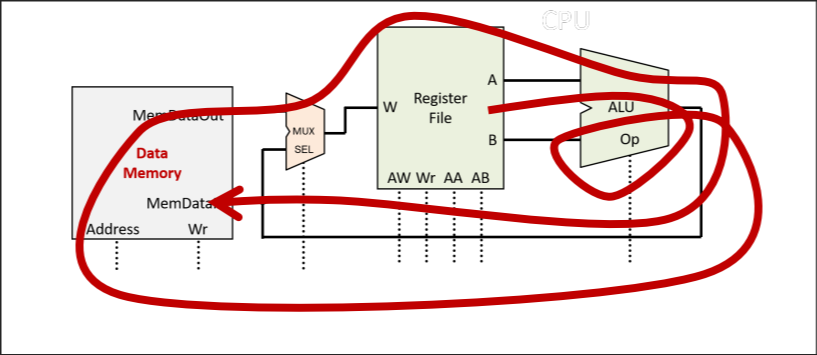
\includegraphics[scale=0.2]{screenshots/2025-10-12_9.png}
		\end{center}
We would need to go like four times to the ALU, the fact is that \important{this is possible} however it makes it hard to optimize the processor.
\end{framedremark}
The question behind all this is how does intel can still be as famous as they are now with instruction that looks like this and that cannot really be optimized? There is still the majority of the processor to this day that are intel processor (even if amd is better...), we will see this in a couples of weeks.
\subsubsection{Byte addressed memory}

Almost all ISA today are use byte addressed memory. byte are quite important, disks are organized in bytes, network packets are bytes, \important{ascii} are byte. A lot of data are represented as byte so using an word addressed memory wouldn't be very efficient here, we would either loose a lot of time looking for the right byte, or loosing a lot of space by putting byte in word address (losing the three other bytes).\\
The solution is to no change the way memory is placed \textbf{but} \important{changing the label}.
\begin{center}
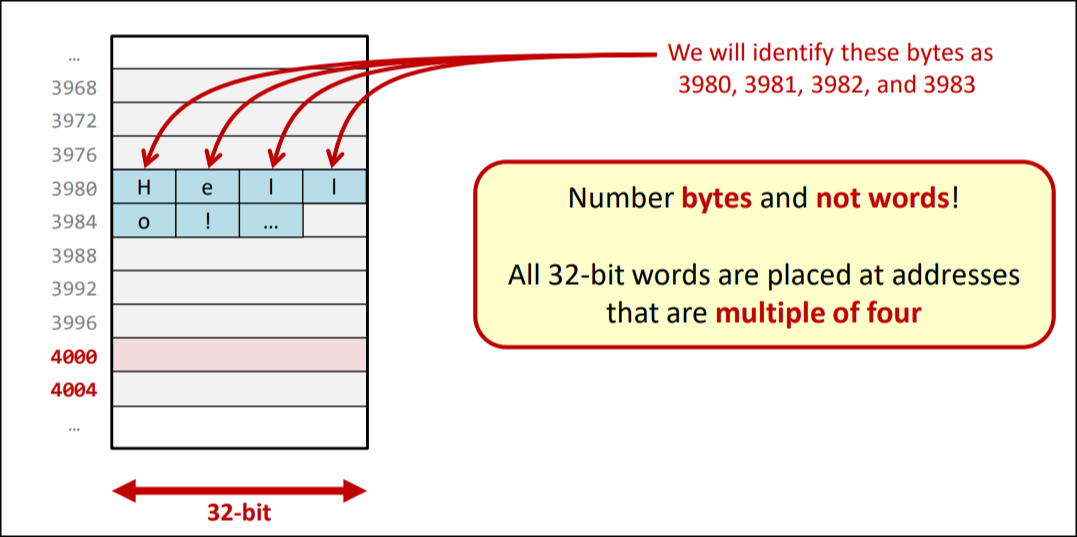
\includegraphics[scale=0.3]{screenshots/2025-10-12_10.png}
\end{center}
\paragraph{Loading a word (\texttt{lw}) and Instruction}%
For instance, if we are interested in word, we cannot look for the word at address 3981, this would'nt be a word.
\begin{center}
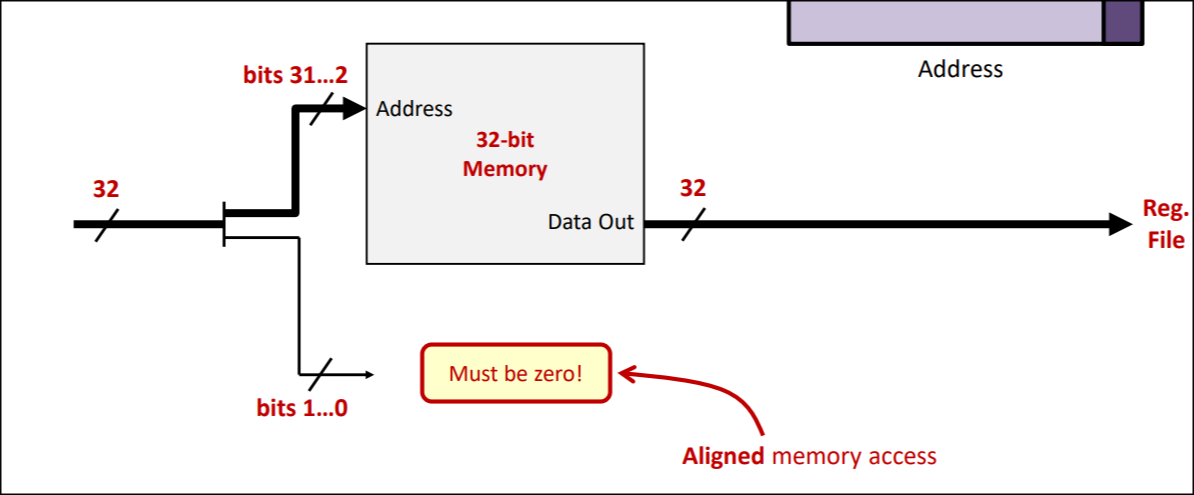
\includegraphics[scale=0.25]{screenshots/2025-10-12_11.png}
\end{center}
As said before when loading a word, it has to be a multiple of 4 so we only care about the 30 most significant bits. The two least significant bits is checked wether there are zero or not and if there are not zero, we would like to \important{throw an exception} which we will see how in a couple of weeks.

\paragraph{Loading byes (\texttt{lb})}%
Here what we are doing is the same as what we did before, we are looking for a word (which is the 30 first bits), and then in the word we choose which 8 bits we wants, this would look like this:
\begin{center}
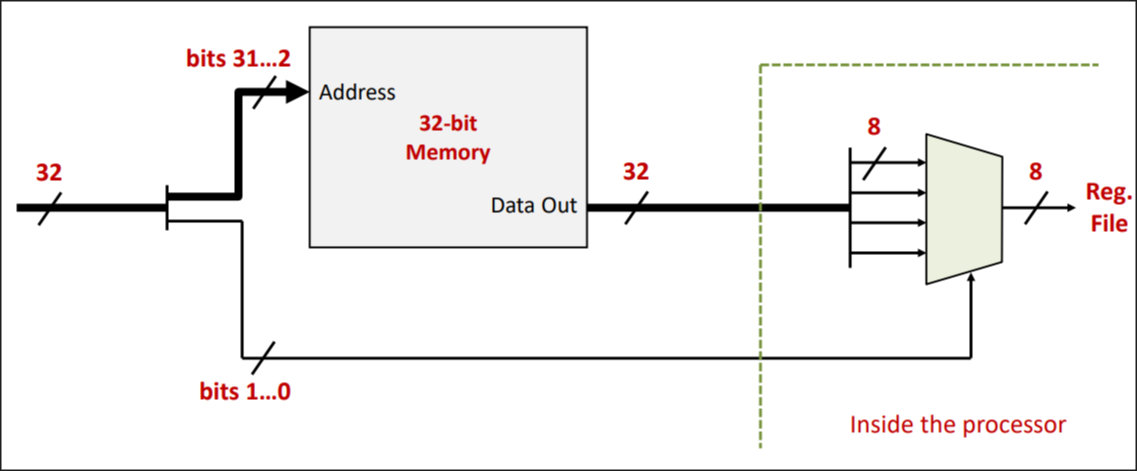
\includegraphics[scale=0.25]{screenshots/2025-10-12_12.png}
\end{center}

Remember when we changed the shape of the memory, how we choose which bit to take; we are doing  the \important{same} here too. The difference is that this part is only in the processor, circuit wise this change nothing.\\
What is good here is that by just adding a multiplexer we can add a lot of instruction in the ISA.

\section{Arrays and data structures}
Data structures is one of the main concept in computer science, even in this course we have already talk about it (the stack).\\
\begin{parag}{Arrays in high-level languages}
	\begin{lstlisting}[language=Scala]
val myData: Array[Short] = Array(10407, -16533, -22715, 123133, 12512)
    \end{lstlisting}
\end{parag}
Here we have a sequence of number that are indexed, the question however is how do we store them.\\
We have a lot of ways to do so (three), we can have a pointer to the first element, and the having the other following this one. With this methode the issue is when does the array stops?\\
One way to do so is to put a \textit{null} element at the end of the array so that we know that this is the end of the array.  The definition of string are in fact an array of char with the 0 char at the end.\\
Another way with this is just to to do nothing. Having a pointer to the start of the array and the hoping t hat the programmer knows what is his doing. \texttt{C} Arrays for instance are built like this.\\
A whole other way is to have, at the start of the array the length of the array. You have a pointer at the start of the array which is the length of the array and then you do your computing as usual
\begin{center}
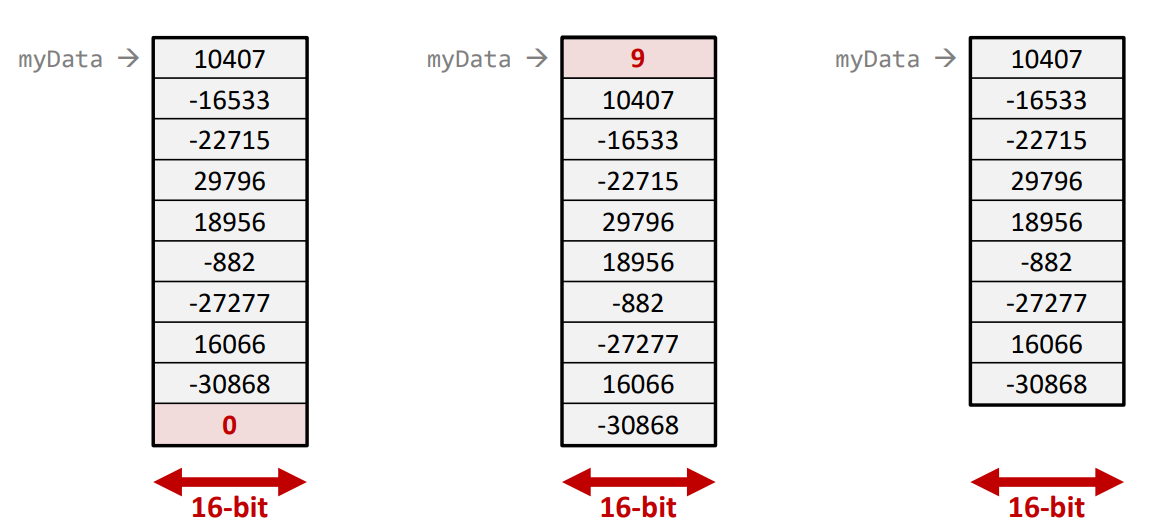
\includegraphics[scale=0.3]{screenshots/2025-10-21.png}
\end{center}
\begin{parag}{Adding Positive elements}
    To add all the positie elements in an array of signed 16-bit integers we would:
	\begin{itemize}
	    \item At call time, \texttt{a0} points to the array (and, in type 3, \texttt{a1} is the length)
	    \item At return time, \texttt{a0} contain the result
	\end{itemize}
	The result for the type 3 (written in \texttt{c}):
	\begin{lstlisting}[language=c]
short add_positive(short myData[], int N) {
	short  sum = 0;
	for (int i = 0; i < N; i++) {
		if (myData[i] > 0) {
			sum += myData[i];
		}
	}
	return sum;
}
	\end{lstlisting}
\end{parag}
\begin{parag}{Adding positive elements (Type 1)}
    For the first type let us write the code for this in RISC-V:
	\begin{lstlisting}[language={[RISC-V]Assembler}]
add_positive:
	li t0, 0  #t0 will hold the sum (initialized to 0)

next_short:
	lh t1, 0(a0) # Load short (half-word) at address a0 into t1
	beqz t1, end  # If t1 is 0 (null short) we are done
	bltz t1, negative  # if t1 is negative ignore
	add t0, t0, t1  #Add t1 to the sum (t0)

negative:
	addi a0, a0, 2  # move array pointer (a0) by sizeof(short) to the next element
	j next_short  # repeat the loop
end:
	mv a0, t0  # move the sum (t0) into a0 as the return value
	ret # Return the caller
	\end{lstlisting}
	
	
\end{parag}

\begin{parag}{Adding positive element Type 2}
	\begin{lstlisting}[language={[RISC-V]Assembler}]
addi_positive:
	li 01, 0 #t0 will hold the sum (initialized to 0)
	lh t1, 0(a0) # t1 will count the elemetnts to process
	add a0, a0, 2  # Move array pointer (a0) to the first real element

next_short:
	beqz t1, end  # If t1 is 0 (no more elements), we are done
	lh t2, 0(a0) # Load short (half-word) at address a0 into t2
	bltz t2, negative # If t2 is negative, ignore
	add t0, t0 t2  # Add t2 to the sum (t0)

negative:
	addi a0, a0, 2 # Move array pointer (a0) by sizeof(short)
	addi t1, t1, -1 # Decrement the counter of elements to process
	j next_short  # repeat the loop
end:
	mv a0, t0 # Move the sum (t0) into a0 as the return value
	ret # Return to caller
\end{lstlisting}

\end{parag}



\begin{parag}{Adding positive element Type 3}
	\begin{lstlisting}[language={[RISC-V]Assembler}]
addi_positive:
	li 01, 0 #t0 will hold the sum (initialized to 0)
	mv t1, a1 # t1 will count the elemnts to process (a1)

next_short:
	beqz t1, end  # If t1 is 0 (no more elements), we are done
	lh t2, 0(a0) # Load short (half-word) at address a0 into t2
	bltz t2, negative # If t2 is negative, ignore
	add t0, t0 t2  # Add t2 to the sum (t0)

negative:
	addi a0, a0, 2 # Move array pointer (a0) by sizeof(short)
	addi t1, t1, -1 # Decrement the counter of elements to process
	j next_short  # repeat the loop
end:
	mv a0, t0 # Move the sum (t0) into a0 as the return value
	ret # Return to caller
\end{lstlisting}

\end{parag}

\begin{parag}{Adding positive elements (variation on c)}
	Let us add positive elements in an array of signed 16-bits integers:
	\begin{itemize}
	    \item At call time, \texttt{a0} points to the arrays and \texttt{a1} is the length of the arr
	    \item At return time \texttt{a0} contains the result
	\end{itemize}
	Write it by incrementing the index of the array:\\
	\begin{lstlisting}[language=c]
int i = 0;
while (i < N) {
	if (myData[i] > 0) {
		...
	}
	i++
}
	\end{lstlisting}
	This is equivalent to:
	\begin{lstlisting}[language=c]
int i;
for (i = 0; i < n; i++) {
	if (myData[i] > 0) {
		...
	}
}
	\end{lstlisting}
	
	Here we see that we have a variable \texttt{i}  which is incremented by one, therefore, the way of doing this if we were to be compiled would be by having a variable that is incremented by 1 in very loop \textbf{then} be multiplied by the sizeof the data (2 bytes).
	\begin{lstlisting}[language={[RISC-V]Assembler}]
addi_positive:
	li t0, 0 #t0 will hold the sum (initialized to 0)
	mv t1, 0 # t1 will hold the array index

next_index:
	beqz t1, end  # If index >= number of elements , we are done
	slli t2, t1, 1  # t2 = offset of the element as index (t1) * sizeof(short)
	add t2, a0, t2 # Address of the element = myData (a0) + offset(t2)
	lh t3, 0(t2) # load short (half-word) at address a0 into t3
	bltz t3, negative #if t3 is negative, ignore
	add t0, t0, t3 # Add t3, to the sum (t0)

negativ:
	addi t1, t1, 1 #Increment the counter of element to process
	j next_index  # repeat the loop
end:
	mv a0, t0 # Move the sum (t0) into a0 as the return value
	ret # Return to caller
	\end{lstlisting}
	
	\begin{subparag}{Which is better}
	    We have now two different way to do the same type (type 3), however which one is faster? this question can be easily answers: the first one that we have written has less intrustion $\implies$ faster. (this is not always that simple)\\
		But this points out an issue, we need \important{good compiler}, we need a compiler that can translated our code into the fastest assembly possible.
	\end{subparag}
\end{parag}


\begin{parag}{Linked list}
    Another way to store data is with a linked list:
	\begin{center}
	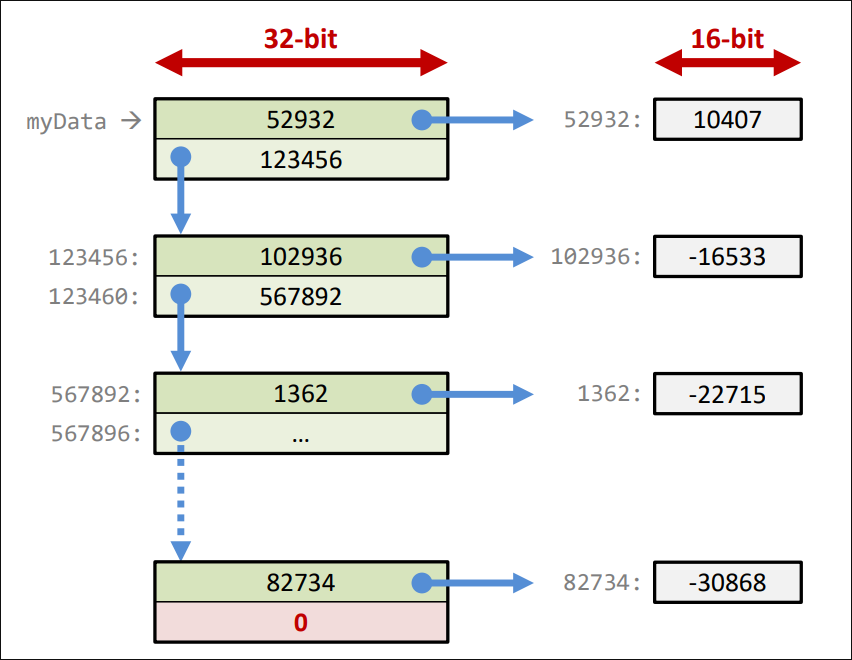
\includegraphics[scale=0.3]{screenshots/2025-10-21_1.png}
	\end{center}
	As we can see here this is the same principle as what we did before, we store for each element the current address of the value \important{and} the address of the next value. To  iterate through this list all we have to do is to go to the current value get the value via the address and then take the next iteration with the second address.\\
	What is good about this is that:
	\begin{itemize}
	    \item  Insert element in the array is very easy
	\end{itemize}
	However there is a lot of bad thing here:
	\begin{itemize}
	    \item For each value we have to use 64 bits of addresses which is a lot 
		\item iterate through the list seems nice however are all the instruction truly equal?	
	\end{itemize}
	For  instance imagine we wanted to recreate the same code as the one we wrote for the other arrays:
	\begin{lstlisting}[language={[RISC-V]Assembler}]
add_positive:
	li t0, 0 # t0 will hold the sum
next_element:
	beqz a0, end # If address of next element (a0) is zero, we are done
	lw t1, 0(a0) # Load address of actual data into t1
	lh t1, 0(t1) # Load short (half-word) at address t1 into t1
	bltz t1, negative # if t1 is negative, ignore 
	add t0, t0, t1  #  Add t1 to the sum (t0)

negative:
	lw a0, 4(a0) # Load address of next element into a0
	j next_index
end: 
	mv a0, t0 # Move the sum (t0) into a0 as the return value
	ret # Return to caller
	\end{lstlisting}
	
	As we can see here: this is not much more complex. but is it more efficient: no. The instruction of loading and storing are way slower than the other instruction, the fact that this way of computing leads to a lot more of load makes it way slower.
	
	
\end{parag}







\section{1.e: Instruction Set architecture Arithmetic}
\begin{parag}{Notation}
    \begin{itemize}
        \item Number (represented on a specific no. of digits/bits)
			\begin{align*} A =  A^{\left(n\right)}  =  A^{\left(m\right)}\end{align*}
		\item  Number (in binary or decimal)
			\begin{align*} A = A_{10} =  A_2 = A_{2c} \end{align*}
			\item Individual digits (bits)
				\begin{align*} a_{n-1}, a_{n-2}, \ldots, a_2, a_1, a_0 \end{align*}
				\item Digit string (representation)
					\begin{align*} <a_{n-1}a_{n-2}\cdots a_2 a_1 a_0> \end{align*}
    \end{itemize}
\end{parag}
\begin{parag}{Numbers}
    we usually care for three types of numbers:
	\begin{itemize}
	    \item \important{Integers} (signed and unsigned)
		\item Fixed point
			\begin{align*} 0.12, 3.14, 1013141212512.5124213 \end{align*}
			\begin{itemize}
			    \item Essentially integers with \important{implicit $10^{k}$ or $2^k$ scaling}
			    \item Extremly important in practice (most signal processing is fixed point)
			\end{itemize}
		\item \important{Floating point}	
			\begin{align*} 3.14E3, -2.4E-1 \end{align*}
	\end{itemize}
	\begin{framedremark}
	As we have seen in it fds, we feel like fixed point are just some useless number representation but this is \important{false}. As said before, in signal processing we use a lot of number that needs to be \textit{pointed} (not integers), but it also need to be \important{fast} as for us to be able to watch a live twitch or a youtube video... We need to do a lot of computation the fastest way possible. Floating point are pretty bad at this, addition using floating is much more slower than integers addition, we know that fixed point are just integers disguised as rational number. That's the reason why we use fixed point representation.
	\end{framedremark}
\end{parag}
\begin{parag}{Unsigned Integers}
    \begin{align*} A = \sum_{i = 0}^{n - 1} a_iR^i \end{align*}
\end{parag}
\begin{framedremark}
For the next part of this course I am gonna skips this because it is a big review of what we have already seen in fds, I am just going to write what I find intresting \textbf{for me} which is not necessarly the most important thing.
\end{framedremark}
\begin{parag}{Addition is unchanged from unsigned}
    As we can see (remember of the table) addition for signed number (in two's complement) and unsigned number is the same, this allows us to have \important{only} two instructions (\texttt{add} and \texttt{sub}) without any \texttt{addu} like instruction.\\
	This is one of the reason why we use 2's complement as the universal representation of signed integers today.
\end{parag}


\begin{parag}{Overflow in hardware}
    In hardware, \important{carry out} is the only missing bit from the \important{complete} result\\
	We can think of overflows as a \important{tuncation} problem:
	\begin{center}
	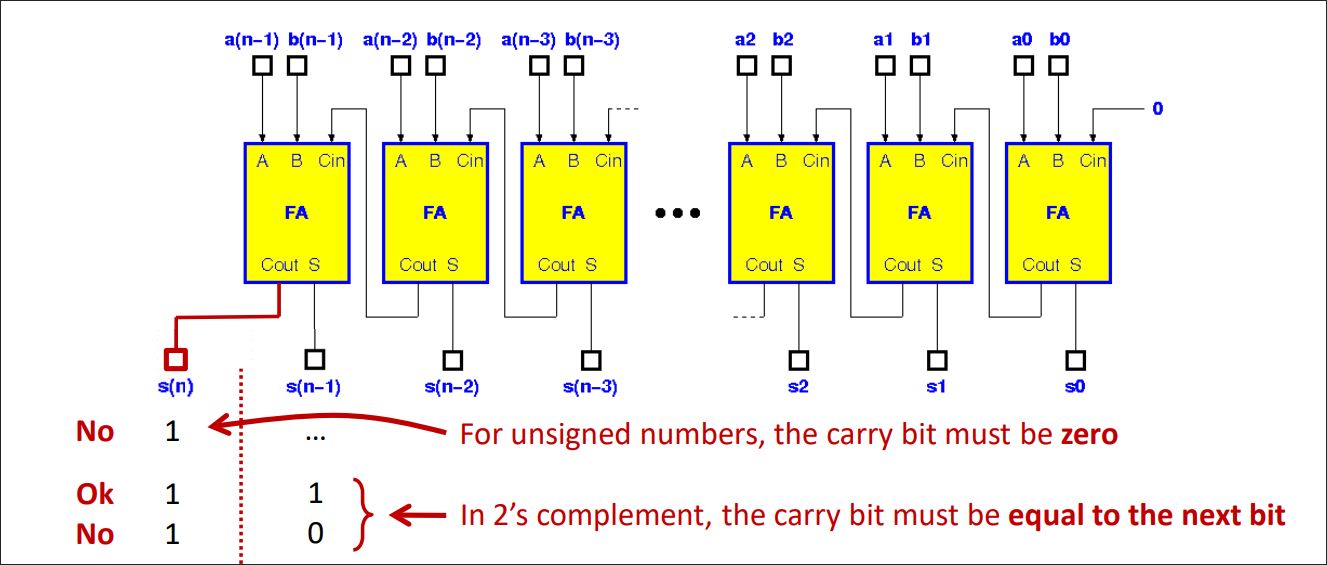
\includegraphics[scale=0.3]{screenshots/2025-10-21_2.png}
	\end{center}
\end{parag}
\begin{parag}{Overflow in software}
    Some architecture (e.g., \important{x86}) gives us the \important{carry bit} in a special register (a \important{flag})
	\begin{center}
	    \textrightarrow overflow detection is the same as in hardware
	\end{center}
	Other modern architecture gives us \important{only the result} of the addition (e.g., \important{RISC-V}). The detection is usually based on the following observations:
	\begin{itemize}
	    \item If addition of \important{opposite sign number} $\implies$ magnitude can only reduce $\to$\important{no overflow possible}
	    \item If addition of \important{same sign number}$\implies$ overflow is possible but the sign of the result will appear wrong.
	\end{itemize}
	
	
	\end{parag}
\begin{parag}{$A + \overline{A} = -1$}
	As we have seen here
	\begin{align*} -A = \overline{A} + 1\end{align*}
	To prove it:
	\begin{align*} &\left(-a_{n-1} 2^{n-1} + \sum_{i =  0}\
		^{n-2}a_i2^i\right) + \left(-\overline{a_{n-1}}2^{n-1} + \sum_{i = 0}^{n-2}\overline{a_i}2^i\right) \\ &= - \left(a_{n-1} + \overline{a_{n-1}}\right) \cdot 2^{n-i} + \sum_{i = 0}^{n-2}\left(a_i + \overline{a_i}\right) \cdot 2^i =  -2^{n-1} + \sum_{i = 0}^{n-2}  2^i\\ &=  -1
\end{align*}
    
\end{parag}
\begin{parag}{Two's complement Add/Subtract Units}
    With this proprety it becomes very easy to compute subtraction as it is just the use of the addition part but with the inverse + 1. This can be done by having a $c_{in}$ at the beggining of the adder and to have a multiplexer to choose between the $b_i$ or $\neg b_i$
	\begin{center}
	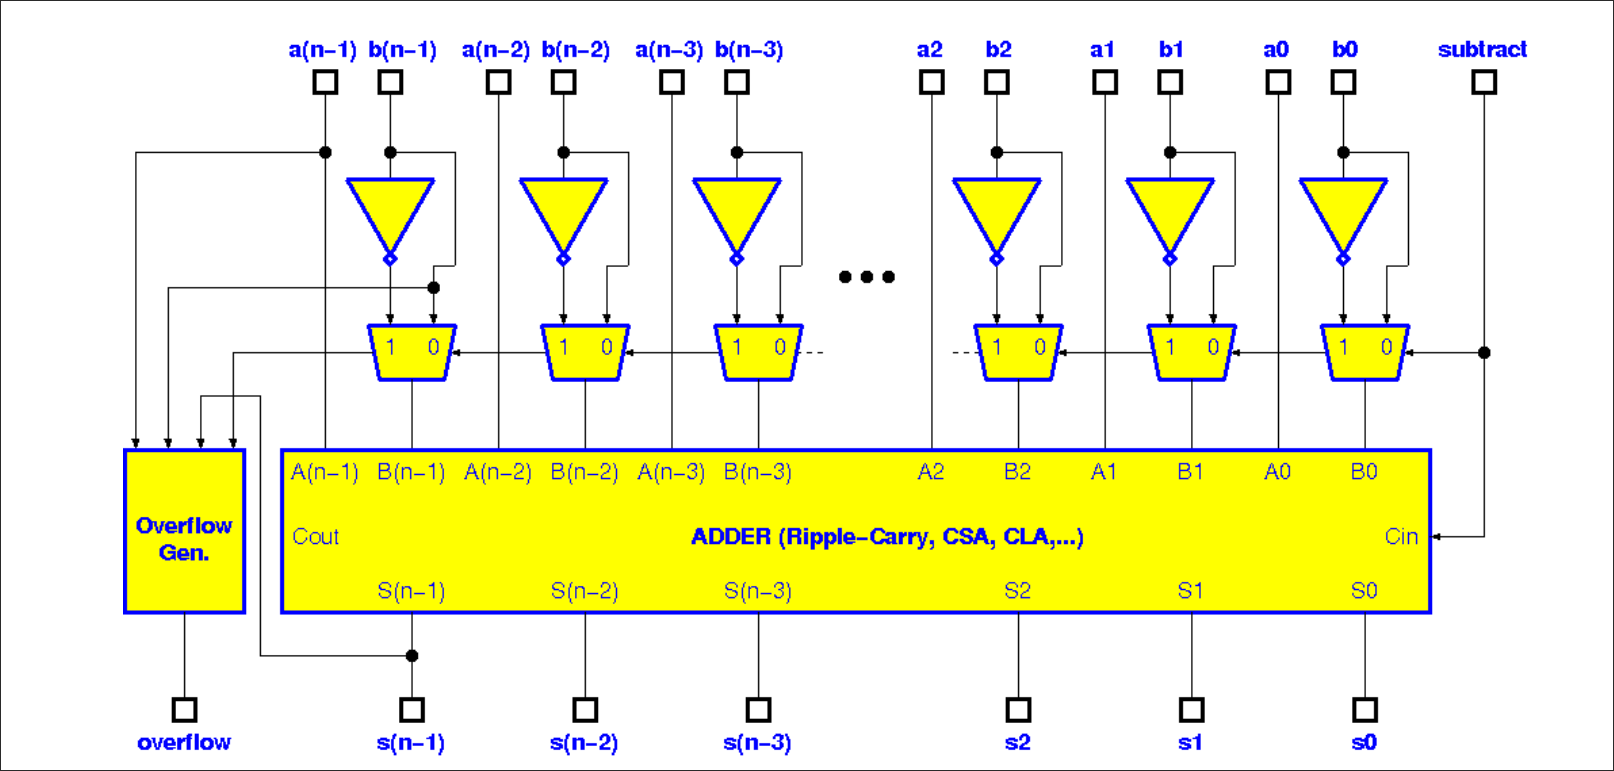
\includegraphics[scale=0.2]{screenshots/2025-10-21_3.png}
	\end{center}
	as we can see this allows us to put the substraction and addition into the same module.
\end{parag}








\chapter{Processors, I/Os, and Exceptions}
\section{2a. Multicycle Processor}
In this section, we will more go into the detail of the \important{hardware} behind the cpu. Especialy multicycle processor.\\
As seen before, the CPU has more than one part:
\begin{center}
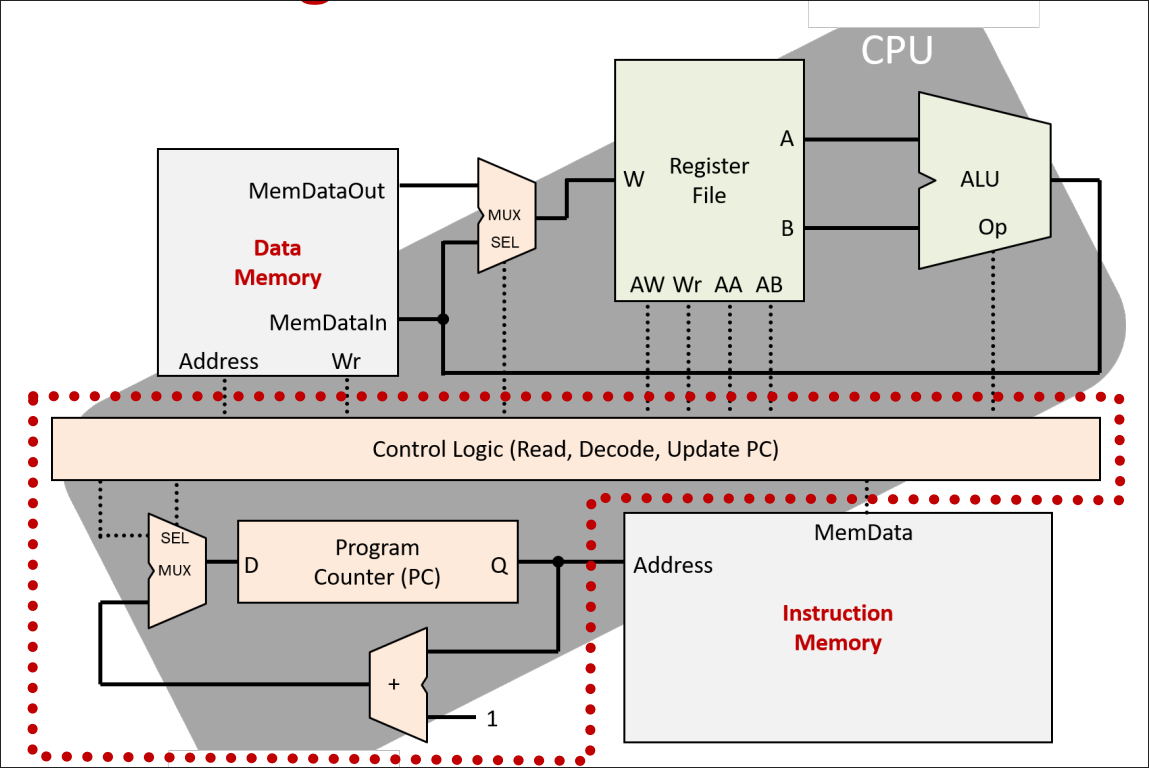
\includegraphics[scale=0.2]{screenshots/2025-10-21_5.png}
\end{center}
However the red part (les pointilles rouges) here is in fact a \important{big finite-state machine}. This means that we can create a state diagram for it.
\begin{parag}{Single cycle processor} For instance the state diagram of a single-cycle processor is very easy: 
\begin{center}
\begin{tikzpicture}[
    state/.style=
	{circle, mininum size=9cm, draw, align=center, ->, >, >=stealth', auto, semithick },
    >=Stealth
]

\node[state]  at (0, 0)(execute) {Execute an\\instruction};
\node[state, right=3cm of execute]at (1, -2) (halt) {Halt};

\draw (execute) edge[loop above] node {PC $\leftarrow$ PC + 4} (exectute);
\draw (halt) edge[loop above] node {not} (halt.west);

\draw[->] (execute) edge[bend left] node {\tt break} (halt);

\end{tikzpicture}
\end{center}
\begin{subparag}{Remark}
    If someone knows how to makes the break here above or below the line I will be curious how.
\end{subparag}
There is only two state which means that every instruction is done at a seperate time (single cycle). This directly implies that the longest \important{combinational path} determines the operating frequncy: \important{critical path}.\\
If we wanted to increase frequency then the critical path would be halved into another cycle.
\end{parag}
\begin{parag}{Two-cycle Processor}
    let us look at the finite state machine of a two cycle processor:
	\begin{center}
	    
	
\begin{tikzpicture}[
    state/.style=
	{circle, mininum size=9cm, draw, align=center, ->, >, >=stealth', auto, semithick },
    >=Stealth
]

% Nodes
\node[state]  at (0, 0)(execute) {Start an\\instruction};
\node[state, right=3cm of execute]at (1, -2) (halt) {Halt};
\node[state, below=2cm of execute] (complete) {Complete the \\ instruction};

% Arrows
% % Loop back arrows
% \draw (execute) edge[bend left] node {not \important{break}} (complete);
% \draw (complete) edge[bend right] node {} (execute);
%
% Break arrow to halt
\draw[->] (execute) edge[bend left] node {\tt break} (halt)
	(execute) edge[bend left] node {not break} (complete)
	 (complete) edge[bend left] (execute);
 \draw[->] (halt) edge[loop below] (halt);
\end{tikzpicture}
\end{center}
The question we must ask now is: Did we gain anything?\\
At the moment not really, before we had 1 instruction \important{per cycle} at frequncy $F$. Now, we have 1 instruction every \important{two cycles} at frequncy $2F$.
\end{parag}
\begin{parag}{Not all paths are born equal}
    That's something sad to say but not all path are born equal, some are slower than other, and this is okay (graine de sarrasins). For instance the \texttt{andi} instruction is much faster than the \texttt{lw} instruction.
\end{parag}
\begin{parag}{Multi cycle Processor}
    




\begin{tikzpicture}[
    stage/.style={
        circle, draw, fill=gray!10,
        minimum size=2cm, align=center
    },
    arrow/.style={
        -{Stealth}, thick
    },
    note/.style={
        rectangle, rounded corners,
        draw=red!70!black, fill=yellow!20,
        very thick, inner sep=10pt, align=left
    }
]

% Nodes (pipeline stages)
\node[stage] (fetch1) {Fetch1};
\node[stage, right=1.8cm of fetch1] (fetch2) {Fetch2};
\node[stage, below right=1.4cm and 1.4cm of fetch2] (decode) {Decode};
\node[stage, below left=1.4cm and 1.4cm of decode] (load1) {Load1};
\node[stage, above left=1.4cm  and 4.6cm of load1] (load2) {Load2};
\node[stage, above left=1.4cm and 1.4cm of load1] (execute) {Execute};

% Arrows between stages
\draw[arrow] (fetch1) edge[bend left] (fetch2);
\draw[arrow] (fetch2) edge[bend left] (decode);
\draw[arrow] (decode) edge[bend left] node[right]{Memory} (load1);
\draw[arrow] (load1) edge[bend left] (load2);
\draw[arrow] (load2)  edge[bend left](fetch1);
\draw[arrow] (decode)  edge[bend left] node[below]{ALU/Branch} (execute);
\draw[arrow] (execute)  edge[bend left](fetch1);

\end{tikzpicture}
\\
The goal here is:
\begin{enumerate}
    \item \important{not} to have \important{too many} stages 
    \item To have paths as \important{balanced} as possible
\end{enumerate}
\end{parag}
\begin{parag}{Mealy or Moore?}
    
\end{parag}
\begin{tikzpicture}[
    block/.style={
        rectangle, rounded corners, draw, thick,
        minimum width=2.6cm, minimum height=1.6cm, align=center
    },
    arrow/.style={-Stealth, thick},
    mybox/.style={
        draw, dashed, rounded corners,
        inner sep=10pt, thick
    },
    labelnode/.style={font=\footnotesize\sffamily}
]

%%% --- MEALY MACHINE (TOP) ---
\node[block, fill=red!10, draw=red!60!black] (next) {Next-State\\Logic\\$f_l[\dots]$};
\node[block, fill=blue!10, draw=blue!70!black, right=2.8cm of next] (state) {State\\Memory};
\node[block, fill=cyan!10, draw=cyan!70!black, right=2.8cm of state] (output) {Output\\Logic\\$g_l[\dots]$};

% Inputs/outputs
\node[left=1.2cm of next] (inputs) {Inputs};
\node[right=1.2cm of output] (outputs) {Outputs};
\node[below=1.1cm of next] (clock1) {Clock};

% Arrows
\draw[arrow] (inputs) -- (next);
\draw[arrow] (next) -- node[above,labelnode]{excitation} (state);
\draw[arrow] (state) -- node[above,labelnode]{current state} (output);
\draw[arrow] (output) -- (outputs);

% Feedback arrows (Mealy)
\draw[arrow, red!70!black, very thick] (inputs.north) to[out=70,in=140,looseness=0.8] (output.west);
\draw[arrow, blue!70!black, very thick] (state.east) to[out=-20,in=270,looseness=0.8] (next.south);
\draw[arrow, blue!70!black, thick] (clock1) -| (state.south west);

% Group box
\node[mybox, fit=(next)(state)(output)] (mealybox) {};
\node[below left=0cm and -0.1cm of mealybox.north west, labelnode] {Mealy Machine};

\pgfdeclarelayer{background}
\pgfsetlayers{background,main}
%%% --- MOORE MACHINE (BOTTOM) ---
\node[block, fill=red!10, draw=red!60!black, below=3.2cm of next] (next2) {Next-State\\Logic\\$f_l[\dots]$};
\node[block, fill=blue!10, draw=blue!70!black, right=2.8cm of next2] (state2) {State\\Memory};
\node[block, fill=cyan!10, draw=cyan!70!black, right=2.8cm of state2] (output2) {Output\\Logic\\$g_l[\dots]$};

% Inputs/outputs
\node[left=1.2cm of next2] (inputs2) {Inputs};
\node[right=1.2cm of output2] (outputs2) {Outputs};
\node[below=1.1cm of next2] (clock2) {Clock};
% Group box
\begin{pgfonlayer}{background}
    
\node[below left=0cm and -0.1cm of moorebox.north west, labelnode] {Moore Machine};
\node[mybox, fill=yellow!15, opacity=0.5, fit=(next2)(state2)(output2)] (moorebox) {};
\end{pgfonlayer}{background}



% Arrows
\draw[arrow] (inputs2) -- (next2);
\draw[arrow] (next2) -- node[above,labelnode]{excitation} (state2);
\draw[arrow] (state2) -- node[above,labelnode]{current state} (output2);
\draw[arrow] (output2) -- (outputs2);

% Feedback arrows (Moore)
\draw[arrow, blue!70!black, thick] (state2.east) to[out=-20,in=270,looseness=0.8] (next2.south);
\draw[arrow, blue!70!black, thick] (clock2) -| (state2.south west);

\end{tikzpicture}
I spent an hour on this so please appreciate.\\
\begin{parag}{$\;$}
    The definition of the mealy fsm is that the output depeneds on the \important{input and state}. On the other hand, the definition of the moore fsm is that the output depends on the \important{state only}. \\
	As a human the moore machine is \textbf{way} easier to develop test, etc. We \textbf{always} want to implement a fsm as a moore machine. And good news: it is always possible (almost)\\
	All we have to do is to retard the current output to the next cycle and put our output as a \textit{state} of the fsm. This way: the next output (which becomes the current) is just a \important{state}.

\end{parag}
\subsection{Building the circuit}

    What we are going to do now is to build the circuit. To do so, we'll do it step by step, adding progressiely what we need.\\
	First, we need an instruction register which store the current instruction (so that it doesn't die after one cycle). We will also need a Controller and the \texttt{pc}.\\

\textbf{I-Type instructions Need \texttt{RF} and \texttt{ALU}}\\
	Type I is the instruction with immediate, this means that there is only one value as input (that's why I put value and not values).
    To be able now to \texttt{add}, \texttt{sub}, etc. We need three things:
	\begin{itemize}
	    \item Value to be computed
	    \item Somewhere to compute
	    \item Value to store the result
	\end{itemize}
	The value to be computed and the value to store the result are in the same place: the \important{register file}. The location where we'll compute the instructions are in the ALU (Arithmetic Logic unit)\\

\textbf{R-Type}\\
	we'll go over instructions with two values as input. To do so, we'll use the same ALU as the one before and we'll just add a multiplexer to choose from the immediate and the register value.\\

\textbf{U-Type instructions write an immediate}\\
    We now need to store immediate instead of the result of the ALU. Therefore, those instructions will need a multiplexer \important{after} the \texttt{ALU} in order to choose to write either the result of the \texttt{ALU} or the immediate.\\

\textbf{Load and Store produces a memory address}\\
    For those we will need to output the address. At  the moment the only \textit{load} that we did is on the program with the \texttt{pc}. However now we will also need to load from the memory data. In order to do this, we will need to choose to load either the pc or the output of the \texttt{ALU} as an address $\implies$ we add a multiplexer.\\

\textbf{Loads write the read data into \texttt{RF}}\\
    So now we can access the memory however after accessing the memory we get a \texttt{rdata} which we still need to manage. To do so we will treat it as it is an output from the \texttt{ALU} by \important{adding} a multiplexer. After this output, we will need a signal to know wether we are choosing from memory or from the ALU \texttt{sel\_mem}.\\

\textbf{Stores send an operant to memory}\\
	Now the instruction we want to implement is the \texttt{sw t0, 16(t1)} instruction. For this instruction, we will choose the \texttt{b} signal as the \texttt{t0} and the \texttt{a} as the address(as we did before). Therefore we need to connect the b into the memory with the new signal \texttt{wdata}. The difference between the store and the load is the \texttt{we} (write enable) signal that serve the memory to know wether we are reading or writing into it.\\

\textbf{Branches need to write an offset to the \texttt{PC}}\\
	 To implement the instruction \texttt{beq t0, t1, 1234}, what we do is to change the \texttt{pc} based on a condition, this condition will be compute in the \texttt{ALU}, the \texttt{alu} will output in his lsb wether or not the \texttt{PC} will be updated.\\
	  If the branch is succesful, we want to replace the current \texttt{PC} by the immediate which leads us to add a path from the controller into the \texttt{PC}, a new branch of the \texttt{imm} signal. The controller has to also informed the \texttt{PC} wether or not we have to enable the writting.\\

	Here we have two clauses:
	\begin{enumerate}
	    \item \texttt{branch\_op} \textrightarrow informs us of if we are in a branch operation 
	    \item \texttt{alu\_res} which is the lsb of the \texttt{ALU} as said before
	\end{enumerate}
	If those two signal are up $\implies$ we enable the write of the \texttt{PC}.
    \begin{framedremark}
    As we can see now, the \texttt{PC} is no longer just a simple register, it contains some logic to compute new values.
    \end{framedremark}
\textbf{jump and link need to store \texttt{PC + 4} in the \texttt{RF}}\\
    To do so, we therefore need another output from the \texttt{PC} which can be stored into the register file based on a signal \texttt{sel\_mem} (whic has to be 0, the inverse of what we have used for before) and the \texttt{sel\_pc} signal.\\
	\begin{center}
	    
	
\scalebox{0.3}{
\begin{circuitikz}
\tikzstyle{every node}=[font=\large]
\draw  (-3.25,30.5) rectangle (3,20.5);
\draw  (-1.25,29.75) rectangle  node {\LARGE Controller} (-1.25,29.75);
\draw  (1.75,29) -- (1.75,29) -- (2.25,29) -- (2.25,29) -- cycle;
\node [font=\Large] at (2,29.75) {sel\_imm};
\node [font=\Large] at (2,28.5) {branch\_op};
\node [font=\Large] at (1.75,28) {rf\_we};
\node [font=\Large] at (1.75,27.5) {sel\_addr};
\node [font=\Large] at (1.75,27) {sel\_b};
\node [font=\Large] at (2,26.5) {sel\_mem};
\node [font=\Large] at (1.75,26) {pc\_en};
\node [font=\Large] at (1.75,25.5) {pc\_sel\_pc\_base};
\node [font=\Large] at (1.5,24.75) {pc\_add\_imm};
\node [font=\Large] at (1.5,24.25) {pc\_sel\_alu};
\node [font=\Large] at (1.75,23.5) {sel\_pc};
\node [font=\Large] at (2,23) {we};
\node [font=\Large] at (2,22.5) {op\_alu};
\node [font=\Large] at (0.75,21) {imm};
\node [font=\Large] at (-1,21) {ir\_en};
\node [font=\Large] at (-2.25,24) {instruction};
\node [font=\Large] at (-2.5,25.5) {rst\_n};
\node [font=\Large] at (-2.5,27.25) {clk};
\draw (3,29.75) to[short] (4.25,29.75);


\draw (7.25,29.75) to[short] (7.5,29.75);
\draw (7.25,29.25) to[short] (7.5,29.25);
\draw (7.5,29.75) node[ieeestd and port, anchor=in 1, scale=0.89](port){} (port.out) to[short] (9.25,29.5);
\draw [ line width=1.7pt](3,29.75) to[short] (7.5,29.75);
\draw [ line width=1.7pt](6.75,29.25) to[short] (7.25,29.25);
\node [font=\Large] at (6,29.25) {alu\_res};
\draw [ line width=1.7pt](3,26) to[short] (10.75,26);
\draw [ line width=1.7pt](10.75,26) to[short] (10.75,29);
\draw [ line width=1.7pt](9.25,29.5) to[short] (10.75,29.5);
\draw (12.5,29.5) to[short] (12.75,29.5);
\draw (12.5,29) to[short] (12.75,29);
\draw (12.75,29.5) node[ieeestd or port, anchor=in 1, scale=0.89](port){} (port.out) to[short] (14.5,29.25);
\draw [ line width=1.7pt](10.75,29) to[short] (12.5,29);
\draw [ line width=1.7pt](10.75,29.5) to[short] (12.75,29.5);
\draw [ line width=1.7pt ] (16.75,31.75) rectangle (23.5,18.5);
\draw [ line width=1.7pt ] (20.5,24.75) rectangle  node {\Huge PC} (20.5,24.75);
\node [font=\Large] at (17.75,31) {clk};
\node [font=\Large] at (17.5,30.25) {rst\_n};
\node [font=\Large] at (17.75,27.5) {};
\node [font=\Large] at (18.25,26.75) {sel\_pb\_base};
\node [font=\Large] at (18.25,26) {add\_imm};
\node [font=\Large] at (18,24.75) {imm};
\node [font=\Large] at (17.75,24.25) {sel\_alu};
\node [font=\Large] at (17.75,23.5) {alu};
\node [font=\Large] at (17.25,29.5) {en};
\draw [ line width=1.7pt](14.5,29.25) to[short] (16.75,29.25);
\draw [ line width=1.7pt](16.75,30.25) to[short] (15.5,30.25);
\draw [ line width=1.7pt](16.75,31.25) to[short] (15.5,31.25);
\draw [ line width=1.7pt](3,25.75) to[short] (15,25.75);
\draw [ line width=1.7pt](16.75,26.75) to[short] (15,26.75);
\draw [ line width=1.7pt](15,26.75) to[short] (15,25.75);
\draw [ line width=1.7pt](16.75,26) to[short] (15.5,26);
\draw [ line width=1.7pt](3,25) to[short] (15.5,25);
\draw [ line width=1.7pt](15.5,26) to[short] (15.5,25);
\draw [ line width=1.7pt](3,24.25) to[short] (16.75,24.25);
\node [font=\Large] at (22.25,19.25) {addr};
\draw [ line width=1.7pt ] (3.25,12.75) rectangle (17.75,4.75);
\draw [ line width=1.7pt ] (-6.25,16) rectangle (-2.25,10.75);
\draw [ line width=1.7pt ] (-4.5,13.75) rectangle  node {\Huge IR} (-4.5,13.75);
\draw [ line width=1.7pt ] (10,8.75) rectangle  node {\Huge Register File} (10,8.75);
\node [font=\Large] at (16.75,11.25) {a};
\node [font=\Large] at (16.75,6.75) {b};
\draw [ line width=1.7pt](21.75,8.25) -- (22.25,8.25);
\draw [ line width=1.7pt](21.75,7.75) -- (22.25,7.75);
\draw [ line width=1.7pt] (22.25,8.75) -- (22.25,7.25) -- (23.25,7.75) -- (23.25, 8.25) -- (22.25,8.75);
\draw [ line width=1.7pt](23.25,8) -- (23.75,8);
\draw [ line width=1.7pt](22.75,9.25) -- (22.75,8.64);
\node [font=\Large] at (22.75,8) {};
\draw [ line width=1.7pt](17.75,6.75) to[short] (21.75,6.75);
\draw [ line width=1.7pt](21.75,7.75) to[short] (21.75,6.75);
\draw [ line width=1.7pt](21.75,8.25) to[short] (19.75,8.25);
\draw [ line width=1.7pt](19.75,8.25) to[short] (19.75,15);
\draw [ line width=1.7pt](19.75,15) to[short] (6.25,15);
\draw [ line width=1.7pt](0.75,20.5) to[short] (0.75,15);
\draw [ line width=1.7pt](6.25,15) to[short] (0.75,15);
\draw [ line width=1.7pt](16.75,25) to[short] (16,25);
\draw [ line width=1.7pt](16,25) to[short] (16,15);
\draw [ line width=1.7pt](16.75,23.5) to[short] (15,23.5);
\node [font=\Large] at (14.25,23.75) {alu\_res};
\node [font=\Large] at (22,9.5) {sel\_b};
\draw [ line width=1.7pt ] (24.75,12.25) rectangle (28.5,6.5);
\draw [ line width=1.7pt ] (26.75,9.75) rectangle  node {\Huge ALU} (26.75,9.75);
\draw [ line width=1.7pt](23.75,8) to[short] (24.75,8);
\draw [ line width=1.7pt](17.75,11.25) to[short] (24.75,11.25);
\draw [ line width=1.7pt](26.75,12.25) to[short] (26.75,14.75);
\node [font=\Large] at (26,14.75) {op\_alu};
\draw [ line width=1.7pt](28.5,9.5) to[short] (32.5,9.5);
\draw [ line width=1.7pt](32.5,9.75) -- (33,9.75);
\draw [ line width=1.7pt](32.5,10.25) -- (33,10.25);
\draw [ line width=1.7pt] (33,9.25) -- (33,10.75) -- (34,10.25) -- (34, 9.75) -- (33,9.25);
\draw [ line width=1.7pt](34,10) -- (34.5,10);
\draw [ line width=1.7pt](33.5,8.75) -- (33.5,9.64);
\node [font=\Large] at (33.5,10) {};
\draw [ line width=1.7pt](32.5,10) to[short] (32.5,9.5);
\draw [ line width=1.7pt](32.5,10.25) to[short] (30.5,10.25);
\node [font=\Large] at (30.5,10.75) {imm};
\node [font=\Large] at (33.25,8.5) {sel\_imm};
\draw [ line width=1.7pt](38.25,9.5) -- (38.75,9.5);
\draw [ line width=1.7pt](38.25,10) -- (38.75,10);
\draw [ line width=1.7pt] (38.75,9) -- (38.75,10.5) -- (39.75,10) -- (39.75, 9.5) -- (38.75,9);
\draw [ line width=1.7pt](39.75,9.75) -- (40.25,9.75);
\draw [ line width=1.7pt](39.25,8.5) -- (39.25,9.39);
\node [font=\Large] at (39.25,9.75) {};
\draw [ line width=1.7pt](34.5,10) to[short] (38.25,10);
\draw [ line width=1.7pt](22.25,18.5) to[short] (22.25,16);
\draw [ line width=1.7pt](22.25,16) to[short] (29,16);
\draw [ line width=1.7pt](29,16) to[short] (29,8.75);
\draw [ line width=1.7pt](29,8.75) to[short] (29,7.5);
\draw [ line width=1.7pt](29.25,7.5) to[short] (31.75,7.5);
\draw [ line width=1.7pt](29.5,7.5) to[short] (29,7.5);
\draw [ line width=1.7pt](32.25,7.25) -- (32.75,7.25);
\draw [ line width=1.7pt](32.25,7.75) -- (32.75,7.75);
\draw [ line width=1.7pt] (32.75,6.75) -- (32.75,8.25) -- (33.75,7.75) -- (33.75, 7.25) -- (32.75,6.75);
\draw [ line width=1.7pt](33.75,7.5) -- (34.25,7.5);
\draw [ line width=1.7pt](33.25,6.25) -- (33.25,7.14);
\node [font=\Large] at (33.25,7.5) {};
\draw [ line width=1.7pt](31.75,7.75) to[short] (32.75,7.75);
\draw [ line width=1.7pt](31.75,7.5) to[short] (31.75,8);
\draw [ line width=1.7pt](34.25,7.5) to[short] (38,7.5);
\draw [ line width=1.7pt](38,7.5) to[short] (38,9.5);
\draw [ line width=1.7pt](38,9.5) to[short] (38.75,9.5);








\node [font=\Large] at (33.25,6) {sel\_mem};



\draw [ line width=1.7pt](40,9.75) to[short] (43.75,9.75);
\draw [ line width=1.7pt](43.75,9.75) to[short] (43.75,4.5);
\draw [ line width=1.7pt](43.75,4.5) to[short] (23.5,4.5);
\draw [ line width=1.7pt](23.5,4.5) to[short] (19.75,4.5);
\draw [ line width=1.7pt](19.75,4.5) to[short] (19.75,2);
\draw [ line width=1.7pt](19.5,2) to[short] (1.75,2);
\draw (39,6.5) to[short] (39,6.75);
\draw (39.5,6.5) to[short] (39.5,6.75);
\draw (39,6.75) node[ieeestd or port, anchor=in 1, scale=0.89, rotate=90](port){} (port.out) to[short] (39.25,8.75);
\node [font=\Large] at (39.75,6.25) {sel\_pc};
\draw [ line width=1.7pt](33.25,6.5) to[short] (39,6.5);
\draw [ line width=1.7pt](29.25,9.5) to[short] (29.25,17.25);
\draw [ line width=1.7pt](30.25,17.25) -- (30.75,17.25);
\draw [ line width=1.7pt](30.25,17.75) -- (30.75,17.75);
\draw [ line width=1.7pt] (30.75,16.75) -- (30.75,18.25) -- (31.75,17.75) -- (31.75, 17.25) -- (30.75,16.75);
\draw [ line width=1.7pt](31.75,17.5) -- (32.25,17.5);
\draw [ line width=1.7pt](31.25,16.25) -- (31.25,17.14);
\node [font=\Large] at (31.25,17.5) {};
\draw [ line width=1.7pt](29.25,17.25) to[short] (30.25,17.25);
\draw [ line width=1.7pt](22.25,17.75) to[short] (30.5,17.75);
\node [font=\Large] at (31.25,16) {sel\_addr};
\draw [ line width=1.7pt](32.25,17.5) to[short] (36.75,17.5);
\node [font=\Large] at (4.25,11.75) {clk};
\node [font=\Large] at (4,10.75) {aa};
\node [font=\Large] at (4,9.75) {ab};
\node [font=\Large] at (3.75,8.75) {aw};
\node [font=\Large] at (4,7.75) {wren};
\node [font=\Large] at (4,6.5) {wrdata};
\draw [ line width=1.7pt](1.75,2) to[short] (1.75,6.5);
\draw [ line width=1.7pt](1.75,6.5) to[short] (3.25,6.5);
\draw [ line width=1.7pt](1,7.75) to[short] (3.25,7.75);
\draw [ line width=1.7pt](0.5,8.75) to[short] (3.25,8.75);
\draw [ line width=1.7pt](-2.25,14.75) to[short] (2,14.75);
\draw [ line width=1.7pt](2,14.75) to[short] (2,10.75);
\draw [ line width=1.7pt](2,10.75) to[short] (3.25,10.75);
\draw [ line width=1.7pt](1,14.75) to[short] (1,9.75);
\draw [ line width=1.7pt](1,9.75) to[short] (3.25,9.75);
\draw [ line width=1.7pt](2.5,11.75) to[short] (3.25,11.75);
\draw [ line width=1.7pt](-0.75,14.75) to[short] (-0.75,10.5);
\draw [ line width=1.7pt](-1.5,14.75) to[short] (-1.5,18.25);
\draw [ line width=1.7pt](-1.5,18.25) to[short] (-4.75,18.25);
\draw [ line width=1.7pt](-4.75,18.25) to[short] (-4.75,23.75);
\draw [ line width=1.7pt](-4.75,23.75) to[short] (-3.25,23.75);
\draw [ line width=1.7pt](-9.25,27.75) to[short] (-3.25,27.75);
\draw [ line width=1.7pt](-9.75,25.5) to[short] (-3.25,25.5);
\draw [ line width=1.7pt](-8,15) to[short] (-6.25,15);
\draw [ line width=1.7pt](-7.75,12) to[short] (-6.25,12);
\end{circuitikz}
}
	\end{center}
	I know it is very ugly but this was \important{loong to do}. (for those intrested I used \url{https://tikzmaker.com}, to do it)

\begin{parag}{Detail complex combinational modules}
	As you can guess each part of those module has more into them, for instance the \texttt{ALU} has 4 sub modules (which we will implement in the first part of the second lab).
    \begin{center}
    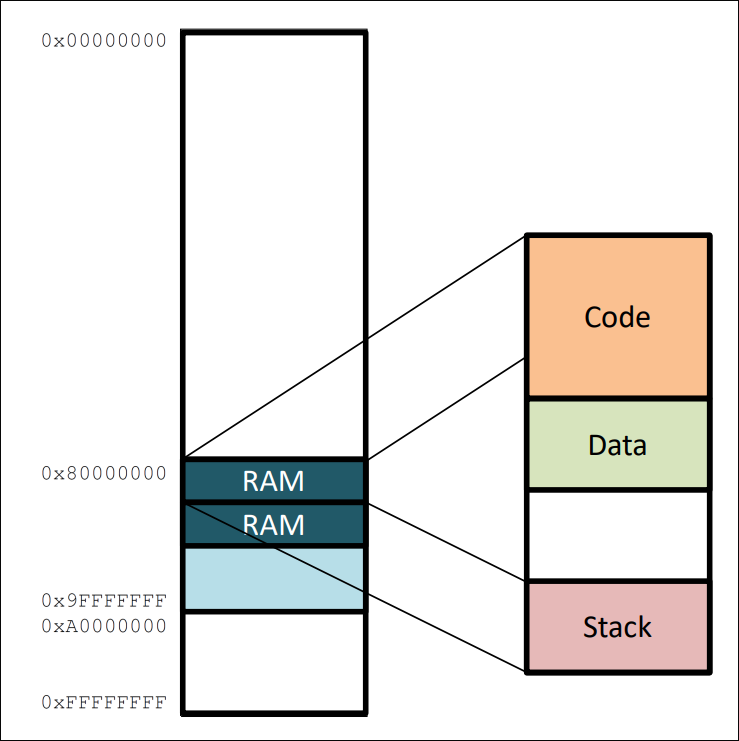
\includegraphics[scale=0.2]{screenshots/2025-10-22_3.png}
    \end{center}
\end{parag}


\section{2b. Processor, Inputs and Outputs}

\begin{parag}{The cpu}
    As said before, the cpu is a very \important{sequential} component (but from now on we may omit the \important{clock} in diagrams). Therefore here we only have one data bus for read and write in our processor. The question we have is how can we handle input and ouput with only one data bus?
\end{parag}
\begin{parag}{Memory}
    At the moment we only need to speak about memory, connecting the cpu with the memory is pretty \textit{easy} as seen before
	\begin{center}
	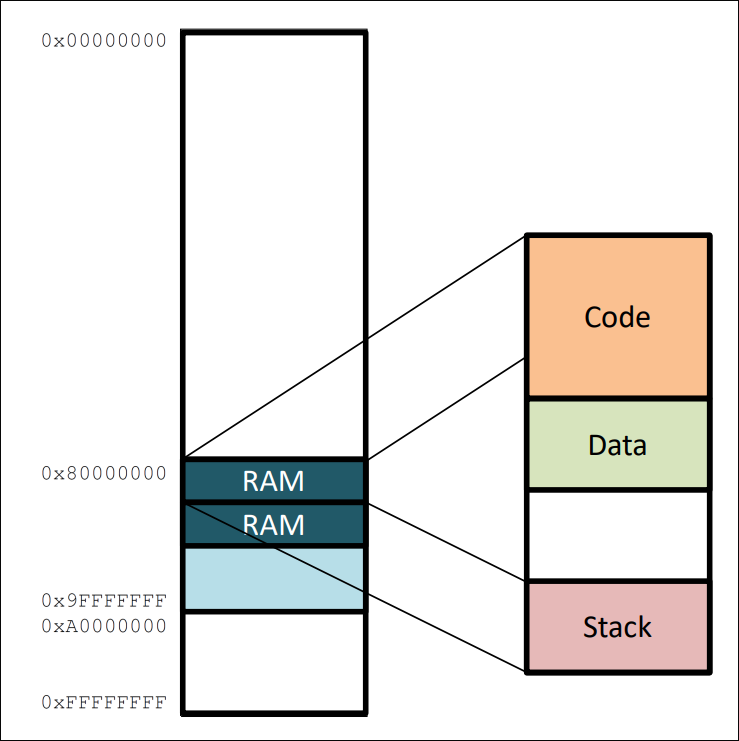
\includegraphics[scale=0.3]{screenshots/2025-10-22_3.png}
	\end{center}
	We assume that the ram begins at the  address \texttt{0x80000000} and then add what is needed to be added:
	\begin{center}
	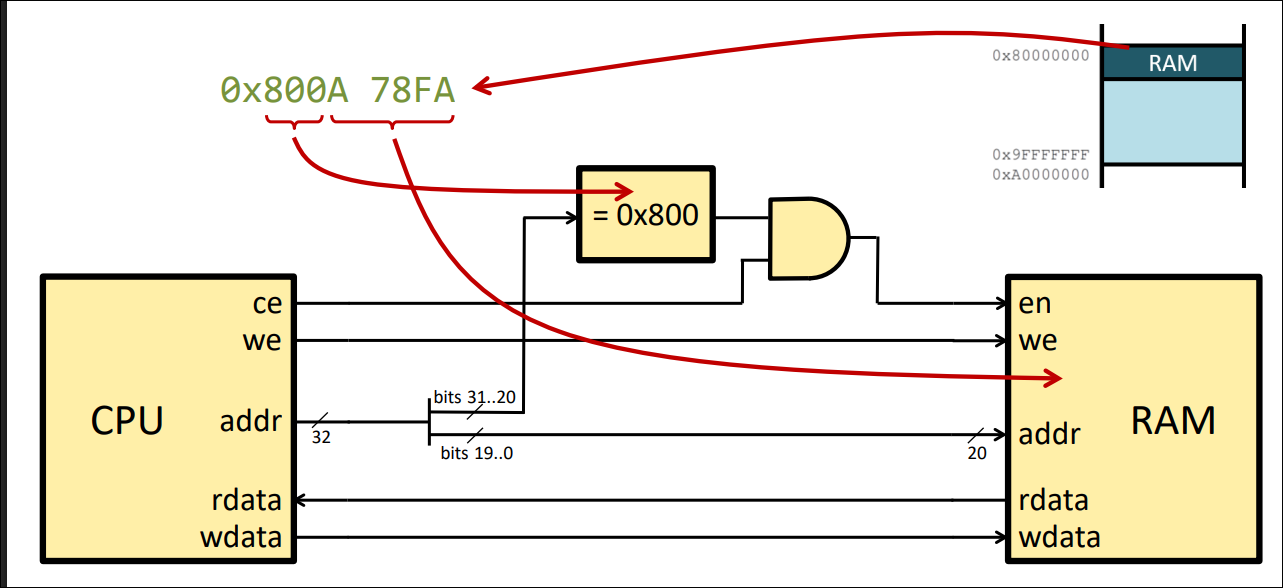
\includegraphics[scale=0.25]{screenshots/2025-10-22_4.png}
	\end{center}
\end{parag}
\begin{parag}{Input and Outputs device}
    As said before we only have 5 classic components of a computer, from where can we get our I/Os then? the way of doing this, is to use memory, we say that the device are just some value in memory with a certain address. However for this we have somme issue:\\
	Some device are way \important{faster} than other for instance here's a table of some examples:
\end{parag}
	\begin{table}[h!]
\centering
\begin{tabular}{|l|l|l|}
\hline
\textbf{Type} & \textbf{Peripheral} & \textbf{Data Rate} \\ \hline
\multirow{2}{*}{Human Interaction} & Keyboard & $\sim$kbps \\
 & Mouse & $\sim$kbps \\ \hline
\multirow{3}{*}{Generic} & Serial Port (RS-232) & 115.2 kbps (max) \\
 & Parallel Port (LPT) & 150 kbps \\
 & USB 4.0 & 20--40 Gbps \\ \hline
\multirow{2}{*}{Generic (Wireless)} & Bluetooth 5.0 & 2 Mbps \\
 & PCIe 4.0 & 16 Gbps per lane \\ \hline
\multirow{2}{*}{Storage} & SATA III (HDD/SSD) & 6.0 Gbps \\
 & NVMe (PCIe 4.0) & 64 Gbps (4-lane) \\ \hline
\multirow{3}{*}{Networking} & Ethernet (10BASE-T) & 10 Mbps \\
 & 10 Gigabit Ethernet (10GBASE-T) & 10 Gbps \\
 & Wi-Fi 6 (802.11ax) & Up to 9.6 Gbps \\ \hline
\multirow{2}{*}{Displays} & VGA (analog video) & 0.6--1.5 Gbps (approx.) \\
 & HDMI 2.1 & 48 Gbps \\ \hline
\multirow{3}{*}{Optical Discs} & CD-ROM & 150 KB/s (1x) -- 7.68 MB/s (52x) \\
 & DVD-ROM & 1.32 MB/s (1x) -- 21.1 MB/s (16x) \\
 & Blu-ray & 4.5 MB/s (1x) -- 54 MB/s (12x) \\ \hline
\end{tabular}
\caption{Approximate data rates for common peripheral interfaces.}
\end{table}
\begin{parag}{Accessing I/Os: Port Mapped I/O (PMIO)}
    The way for this is to create a \important{new interface} similar to the memory one.\\
	We add the to CPU the port \texttt{ctrl-IO} and \texttt{port} Which serves as circuit enable and output enable. (this way, we'll know when accessing memory or I/O).\\
	It implies that we can create new instructions (e.g., \important{x86} but seldom used):
	\begin{itemize}
	    \item \texttt{IN register, port}
		\item \texttt{OUT port, register}
		\item For instance \texttt{IN al, Keyboard}
	\end{itemize}
\end{parag}
\begin{parag}{Accessing I/Os: Memory Mapped I/O (MMIO)}
    In this way, we don't make any difference between memory and I/Os.
	\begin{center}
	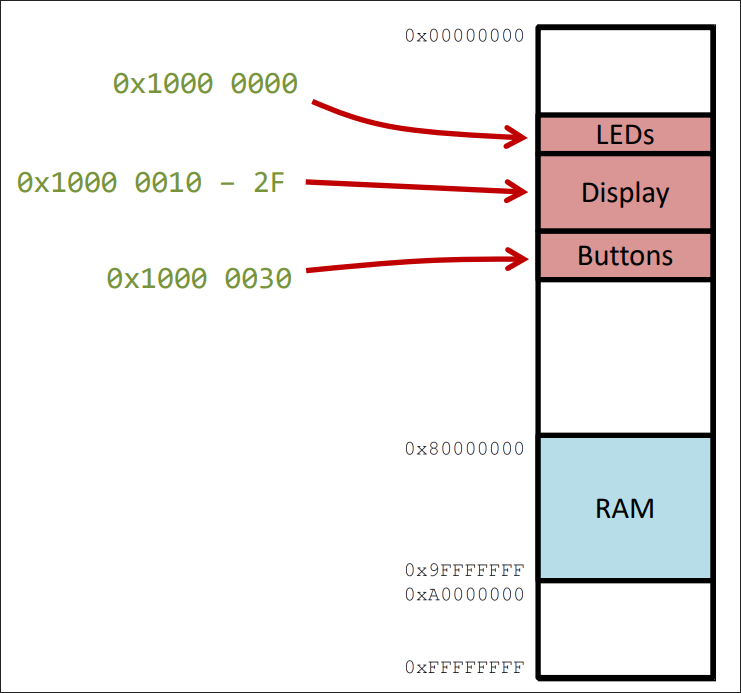
\includegraphics[scale=0.2]{screenshots/2025-10-22_5.png}
	\end{center}
	This means that there are no special hardware needed in the cpu $\implies$ no special instructions needed. For intsance in our example if we wanted to write a new value in the led:
	\begin{lstlisting}[language={[RISC-V]Assembler}]
lui t0, 0x10000 # pointer to I/Os
sw t1, 0(t0) # write LEDs
	\end{lstlisting}
	This means that we have a big data bus and depending on the value \important{the bus} choose between the Memory and the I/Os:
	\begin{center}
	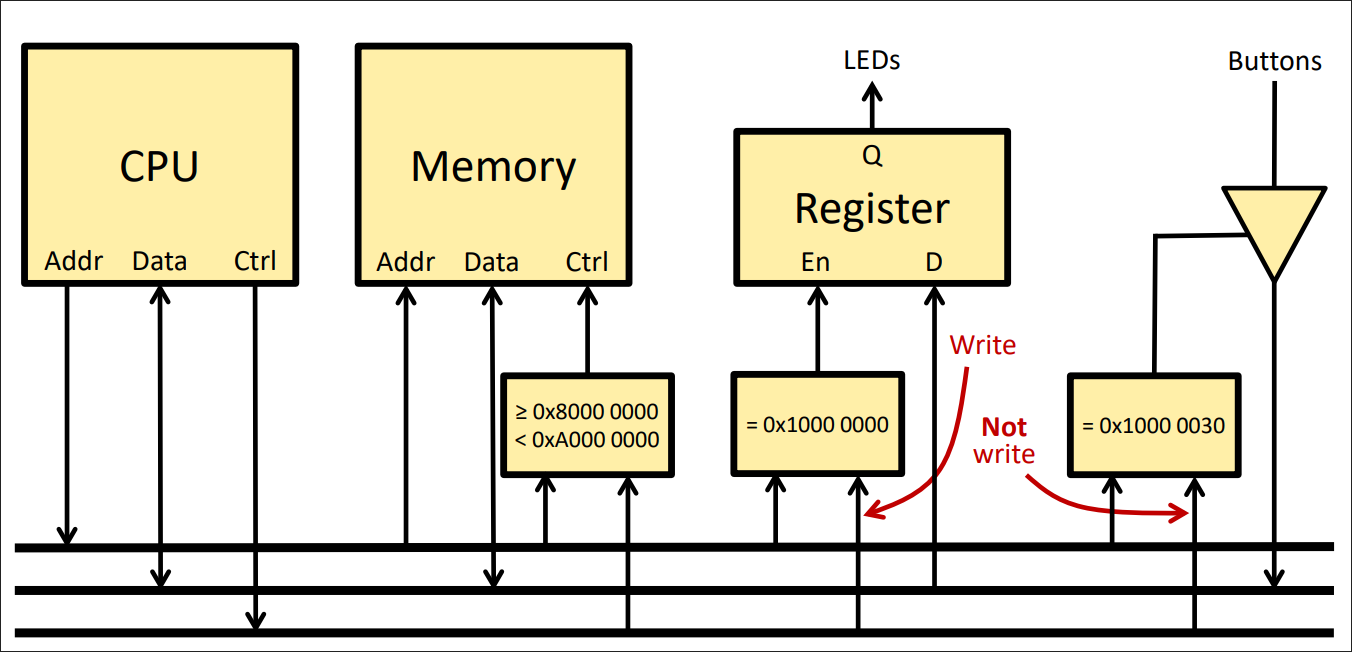
\includegraphics[scale=0.2]{screenshots/2025-10-22_6.png}
	\end{center}
\end{parag}
\begin{parag}{Example: A/D converter}
    An A/D converter is a device that \important{converts an analog signal into a digital signal}. What we need is:
	\begin{enumerate}
	    \item \important{Start} (\texttt{START}): input; when active \textrightarrow begins a new conversion
	    \item \important{Data Valid} (\texttt{/DV}): output when active \textrightarrow D7-D0 are valid
	    \item \important{Data} (D7-D0): output; last conversion result
	\end{enumerate}
	\begin{center}
	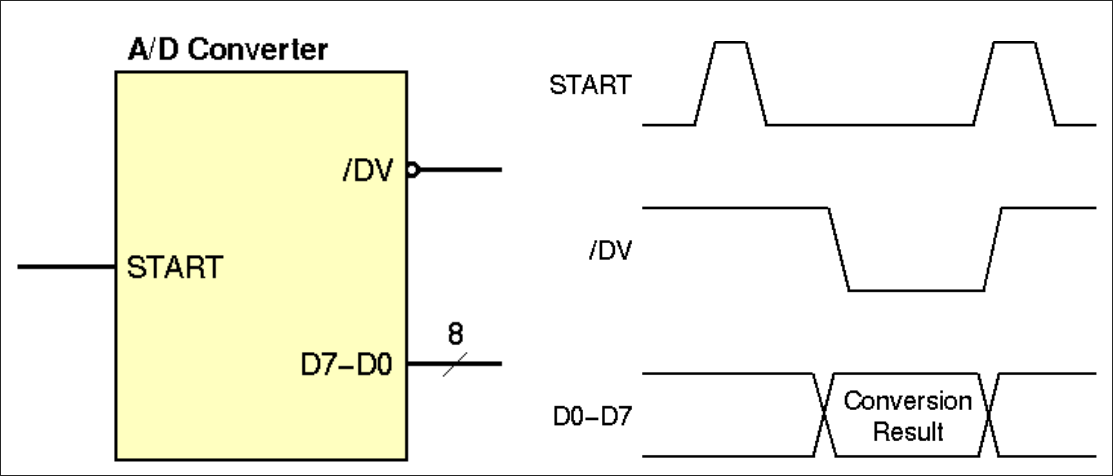
\includegraphics[scale=0.2]{screenshots/2025-10-22_7.png}
	\end{center}
	
\end{parag}


\begin{parag}{Example: Simple bus interface}
    Suppose that a 8-bit processor has the following signals:
	\begin{itemize}
	    \item \important{Address} (A23-A0): output; address bus
		\item \important{Data} (D7-D0): input data bus 
		\item \important{Adress Strobe} (/AS) output, signals the presence of a valid address on the Address bus during a memory access cycle
		\item \important{Read/Write} (R/W): output; signal the direction of the data flow
		\item \important{Data Acknowledge} (/DTACK): input; must be activated at the end of a memory access, when the written data have been latched or the read data are ready
	\end{itemize}
	This is similar but not identical to the MC6800
	\begin{framedremark}
	ChatGPT on the mc68000:\\
	The MC68000 (also called the Motorola 68000) is a 16/32-bit microprocessor that was very popular in the late 1970s and 1980s. It was used in systems like the original Apple Macintosh, Amiga computers, and early Sun workstations. In your example, it’s mentioned as a reference because the bus signals are similar to those on the 68000, but not exactly the same.\\
	\textbf{in short}: the MC68000 is just a classic CPU used as a reference for teaching how these buses work.
	\end{framedremark}
	
\end{parag}
The goal now for us is to create a circuit that is able to connect the A/D converter to the processor (the MC68000). For this we will use a \important{memory mapped interface}. \\
We want: 
\begin{itemize}
    \item \important{any access} (\texttt{R} or \texttt{W}) to address \texttt{0xFFFF0} starts a \important{new conversion}
    \item The \important{data valid} signal can be read by the processor at address \texttt{0xFFFF4} (bit 0)
    \item The \important{result of the conversion} can be read by the processor at address \texttt{0xFFFF8}
\end{itemize}
Here's a little diagram of the state
\begin{center}
	    
	
\begin{tikzpicture}[
    state/.style=
	{circle, mininum size=0cm, draw, align=center, ->, >, >=stealth', auto, semithick },
    >=Stealth
]

% Nodes
\node[state]  at (0, 0)(execute) {Start memory\\ access};
\node[state] at (-4, 0)(left){};
\node[state] at (4, 0)(right){};

% Arrows
% Loop back arrows
\draw (execute) edge[loop above] node {\texttt{/DTACK} == 1} (exectute);
\draw[->] (execute.west) edge[bend left] node {\texttt{/DTACK} == 0} (left);

\draw[->] (right) edge[bend left] node {\texttt{mem\_type} == 1} (execute.east);
\end{tikzpicture}

\end{center}

To be able to construc the circuit we have to be careful about the timing diagram here; the fact that the ADDR and the /AS responds only at the clock edge gives us the information that we will need a \textit{register} which stores the DTACK signal and then output the As and ADDR signal after. This big register here is the \important{processor}.
\begin{center}
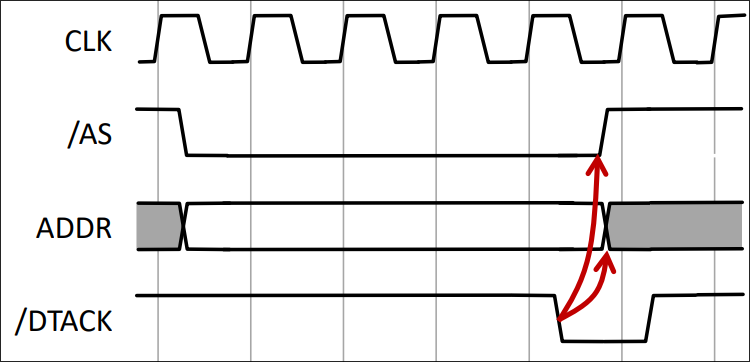
\includegraphics[scale=0.25]{screenshots/2025-10-22_8.png}
\end{center}
	\begin{figure}[h!]
	    \centering
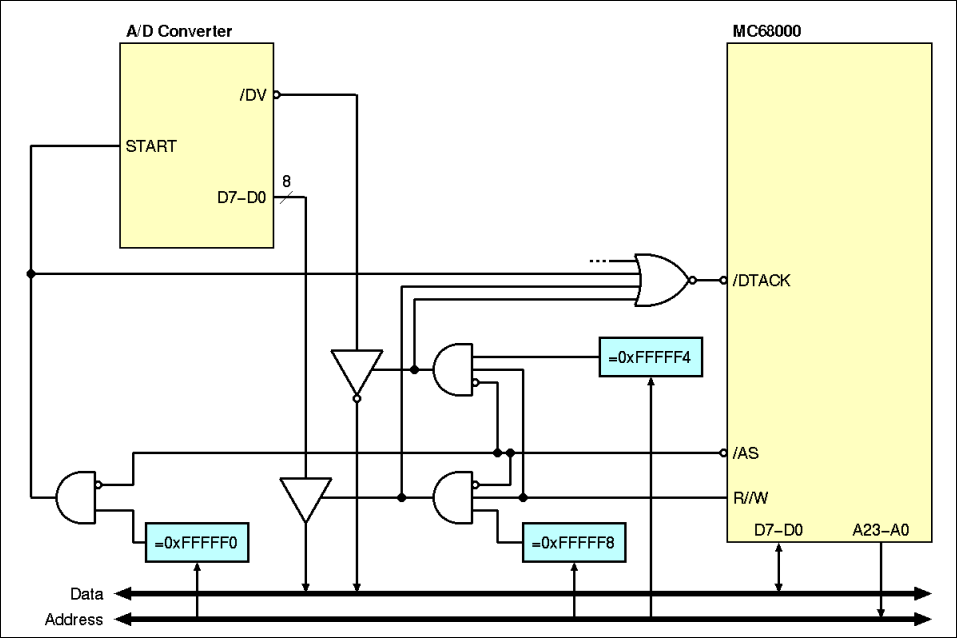
\includegraphics[scale=0.3]{screenshots/2025-10-22_9.png}
\caption{A/D converter circuit}
	\end{figure}
	
\begin{framedremark}
Here we can see that we have two tri-state buffer, but why? It is pretty rare for us to see tri-state buffer so why are they useful here?\\
The answer is that they serve as a multiplexer between the DV and D7-D0, you can look at it and if you think about it, the two tri-state buffers really serve as a \textit{decentralized} multiplexer.
\end{framedremark}

\begin{parag}{A/D converter: software}
    Let us now loot at it as a software person which is pretty easy because of the MMIO:
	\begin{lstlisting}[language={[RISC-V]Assembler}]
read_adc: 
	lui t1, 0xfff 
	addi t1, t1, 0xff0 #t1 = 0xfffff0
	sw zero, 0(t1) # start conversion 
poll:
	lw t0, 4(t1) # t0 = DV signal 
	beqz t0, poll  # wait until done

end:
	lw a0, 8(t1) # a0 = A/D output 
	ret
	\end{lstlisting}
\end{parag}




\begin{parag}{Programmed I/Os}
    \important{Many peripherals} are more developped programmable systems and have a set of registers which the processor reads and writes (a) to \important{send} and \important{receive data} and (b) to \important{issue commands} and \important{read the status}.
	\begin{center}
	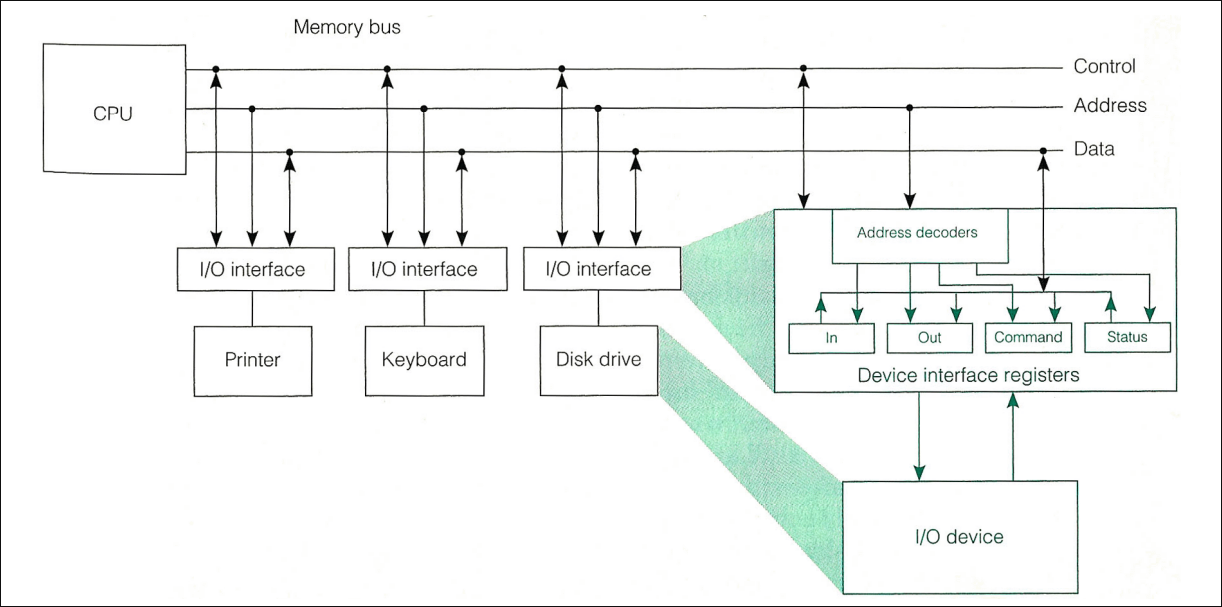
\includegraphics[scale=0.2]{screenshots/2025-10-22_10.png}
	\end{center}
\end{parag}

\subsection{A Classic UART}

\begin{parag}{Definition}
    A \important{UART} means: Universal Asynchronous Receiver-Transmitter\\
	This is one of the \important{simplest and most common communication} peripherals, it is typically used today to connect terminals to embedded devices. Our UART has a \important{simple programmed I/O interface} with four registers:
	\begin{itemize}
	    \item A \important{control register} for the processor to configure the UART 
			\begin{itemize}
				\item Bit 7 must be set to 1 for the UART to be enabled
				\item Bits 2..0 configure the communication speed (e.g., 0b001 for 9600 baud)
			\end{itemize}
		\item a \important{status register} for the processor to check the status of the UART
			\begin{itemize}
				\item Bit 1 is 1 if there are data available
				\item Bit 0 is 1 if the UART is ready to send data
			\end{itemize}
			\item A \important{data input} register where the received  data are available to the processor
			\item A \important{data output} register where the processor places data to send
	\end{itemize}

\end{parag}

\begin{lstlisting}[language={[RISC-V]Assembler}]
UART_CTRL_ADDR = 0x10000000 # UART status register address
UART_ENABLE_BIT = 0x80 # Enable bit (bit 7)
UART_SPEED_9600 = 0x01 # Speed setting for 9600 baud (4 bits, [3:0])
UART_STATUS_ADDR = 0x10000004 # UART status register address
TX_READY_BIT = 0x01 # Transmitter ready bit (bit 0)
UART_DATAIN_ADDR = 0x10000008 # UART data input (receive) register address
UART_DATAOUT_ADDR = 0x1000000C # UART data output (send) register address
send_string:
	li t0, UART_CTRL_ADDR # Get UART control address
	li t1, UART_STATUS_ADDR # Get UART status address
	li t2, UART_DATAOUT_ADDR # Get UART data address
	li t3, UART_ENABLE_BIT # Get enable bit (0x80)
	li t4, UART_SPEED_9600 # Get speed setting (0x01)
	or t4, t3, t4 # Combine enable and speed bits
	sw t4, 0(t0) # Configure using the UART control register
next_char:
	lb t5, 0(a0) # Load first byte of the string
	beqz t5, finish # If byte is zero (null terminator), finish
check_tx_ready:
	lw t6, 0(t1) # Load UART status register
	andi t6, t6, TX_READY_BIT # Check if TX_READY_BIT is set
	beqz t6, check_tx_ready # If not ready, loop back and check again
	sw t5, 0(t2) # Store the character in UART data register
	addi a0, a0, 1 # Increment string pointer (move to next char)
	j next_char # Jump back to send the next character
finish:
	ret # Return when the string is done
\end{lstlisting}
	
	

\begin{parag}{I/O polling}
    Everything we did here is nice however there is still some issue: \important{polling}\\ The issue with polling is that the cpu is \textit{waiting} until the polling is done which is slowing down the cpu (a lot). Moreover, how do we even know if a peripheral has data for us (key pressed, packet arrrived, etc.)? we are not able to polled everything. \\
	For something like a keyboard which would only need to check every ms (approximatively) it would be \textit{okay} however imagine a usb or an ethernet cable this is not managable.
	\begin{center}
	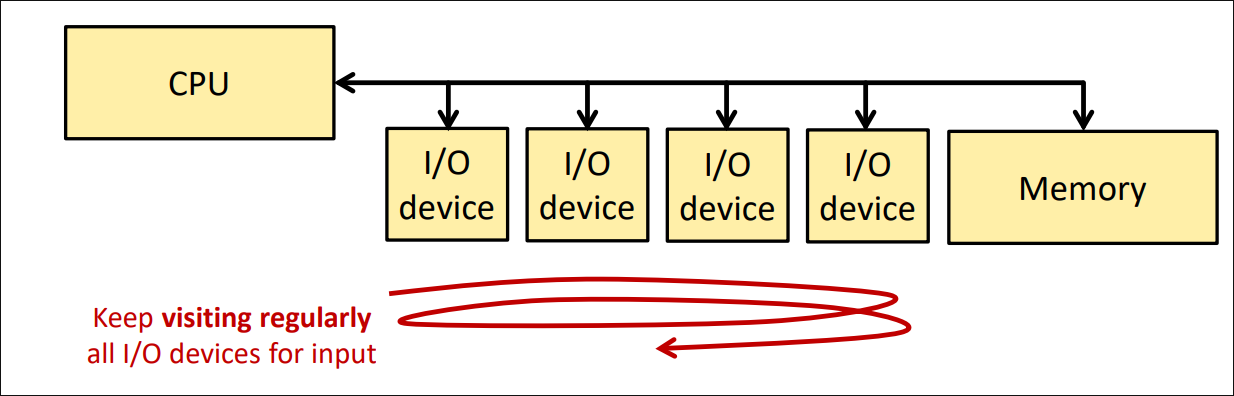
\includegraphics[scale=0.2]{screenshots/2025-10-22_11.png}
	\end{center}
\end{parag}



\section{2c: Interrupts}
The solution of our previous problem is interrupts! Instead of waiting for each I/O to responds, we can do our work and \important{when a I/O} \textit{shouts} we do what he want us to do. We have them \important{ask} for \important{attention}\\
\begin{parag}{Seen this already in some languages}
	We maybe, have already seen this mecanics in some languages:
	\begin{itemize}
	    \item Callbacks, Action, or \important{Event Listeners} (PPO), signals, promises, Futures, Hooks
	\end{itemize}
	However does are done by the \important{compiler}/ \important{interpreters}. Here, we are dealing with the cpu directly so how can we do this?
\end{parag}
\begin{parag}{The basic Idea of I/O interrupts}
    \begin{center}
    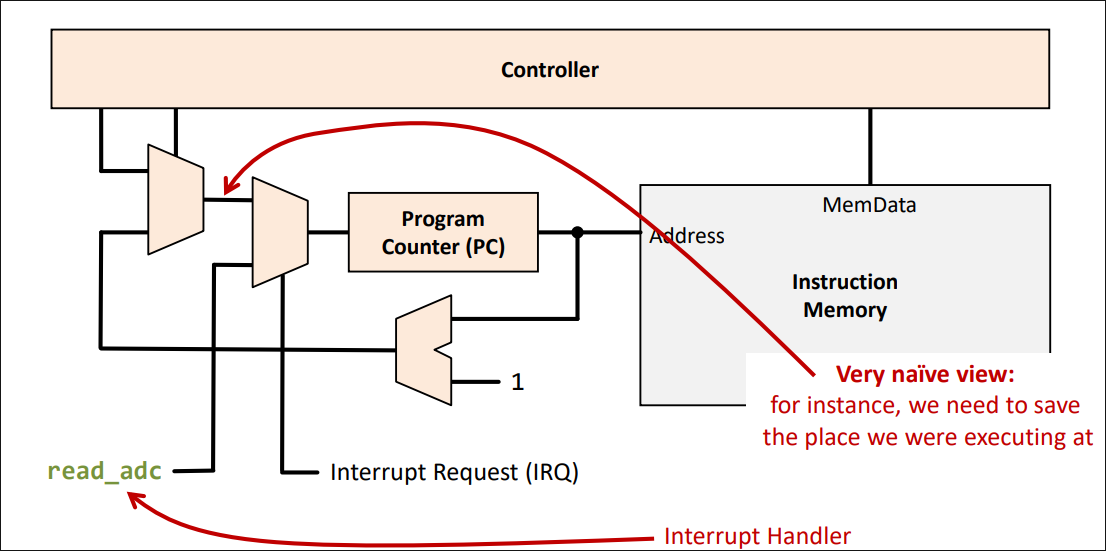
\includegraphics[scale=0.3]{screenshots/2025-10-22_12.png}
    \end{center}
	We use the \texttt{read\_adc} address which is where we handle the I/O interrups. The interrupt request serve to trigger the interruption.\\
	However the is several issues to take care of and behaviours to define:
	\begin{itemize}
	    \item We need to know \important{who needs attention} -- we do not have only one peripheral
			\begin{itemize}
				\item After interrupt, \important{the software checks all peripherals} in turn (polling), or 
				\item \important{I/O peripheral sends identification}
			\end{itemize}
		\item \important{Different priorities} need to be expressed -- some peripheral can wait long, some cannot
		\item \important{Impact on current execution}: Current instruction(s) can complete? One? Five? Twenty? What ahhpens of the program that was executing?
	\end{itemize}
	\begin{subparag}{How do many peripheral connect to a single IRQ}
	    In order to do so, we have more than one way, the easiest and most intuitive is a or with $n$ inputs.\\
		On the other hand, what we also can do is to use tri-state buffers, one for each IRQ$_n$.
	\end{subparag}
	\begin{center}
	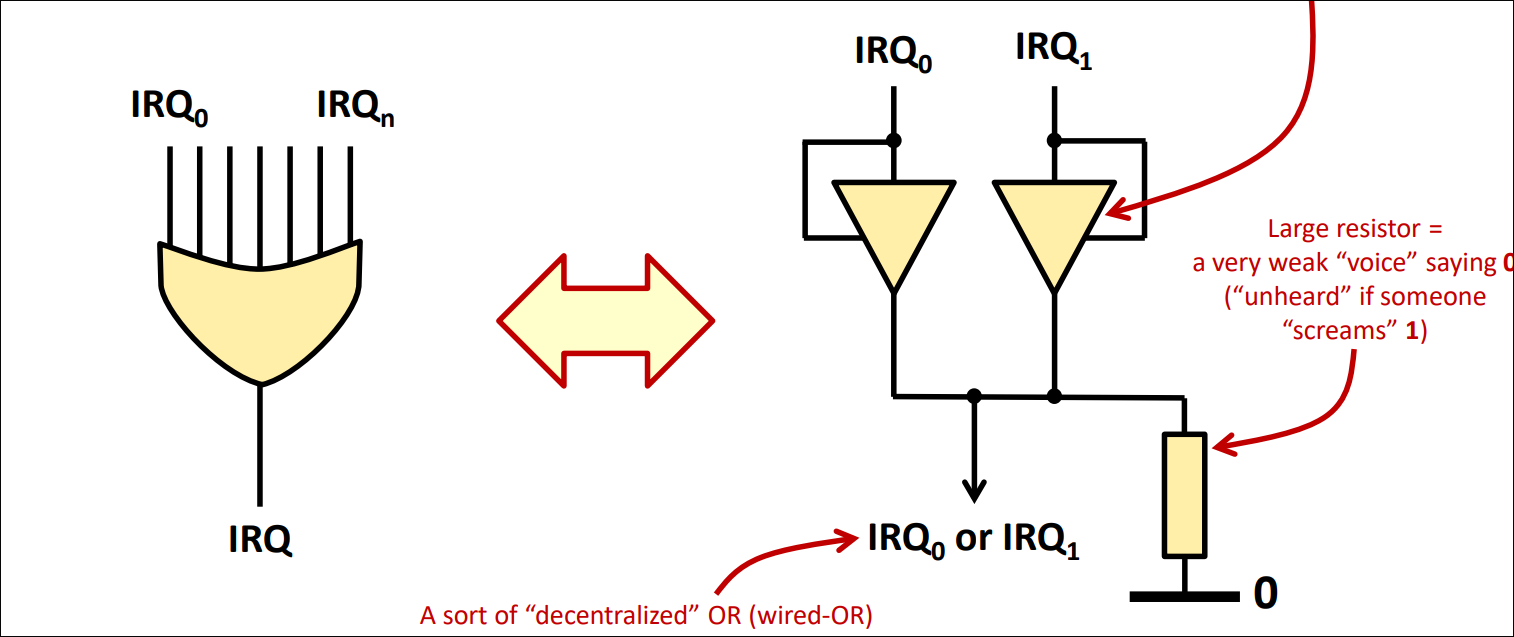
\includegraphics[scale=0.2]{screenshots/2025-10-22_13.png}
	\end{center}
	\begin{subparag}{Example sequence}:
	    \begin{enumerate}
	        \item peripheral asks for attention through IREQ
	        \item Processor signals when it is ready to serve peripheral through IACK "\textit{acknowledges}" the interrupt)
	        \item peripheral signals its identity
	        \item Processor takes appropriate action --transfer control to the appropriate Exception handler
	        \item Processor reverts to the interrupt task
	    \end{enumerate}
	
	\end{subparag}
\end{parag}
		\begin{figure}[h!]
		    \centering
			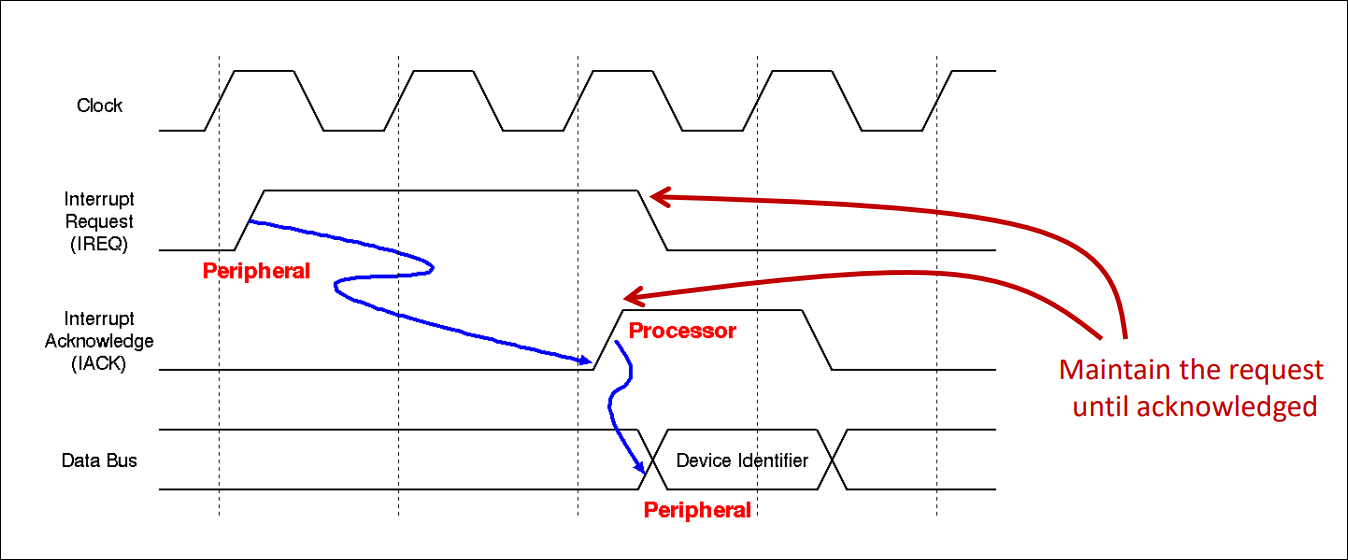
\includegraphics[scale=0.2]{screenshots/2025-10-22_14.png}
			\caption{tiaming diagram}
		\end{figure}
\begin{framedremark}
	On the software side, it works with the same code we used before for polling. However, the \texttt{read\_adc} function is now called by the interrupt handler. The interrupt handler stores the address of the program that manages all interrupt requests, and from there, it launches the program that handles the ADC.
\end{framedremark}
\begin{framedremark}
It is a very good practice to just look at the timing diagram and "\textit{guess}" how the circuit would look like.
\end{framedremark}
\begin{parag}{I/O Interrupt priorities}
    \important{Daisy chain arbitration} is one of the simplest methods:
	\begin{itemize}
	    \item Anyone places request (IREQ, Request)
	    \item Acknowledge line (IACK, Grant) passed from one device to the next 
	    \item Device which wants access, intercepts the signal and hides it from successice devices 
	    \item Simple but (1) slow and (2) hard priorities (meaning hard in like hardcode something).
	\end{itemize}
	\begin{center}
	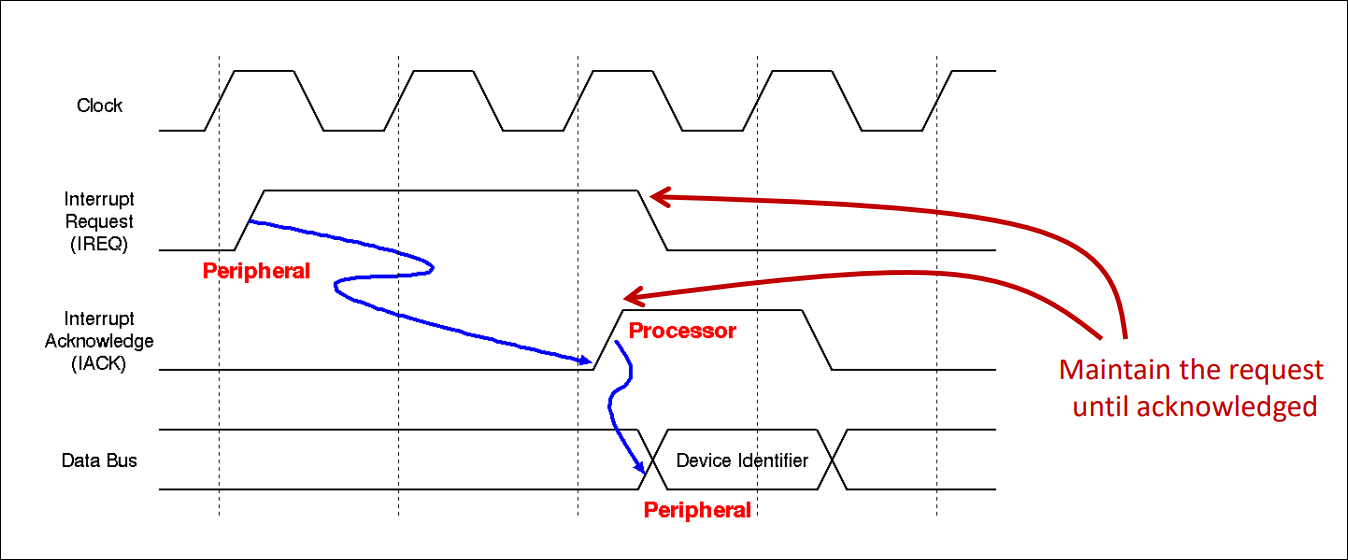
\includegraphics[scale=0.2]{screenshots/2025-10-22_14.png}
	\end{center}
\end{parag}
\begin{parag}{Interrup controller}
	More sophisticated methods involve special hardware:\\
	An \important{interrupt controller}  may be expected to:
	\begin{itemize}
		\item Propagate only one \texttt{IREQ} at a time to the processor 
			\begin{itemize}
			    \item Select the one with highest fixed priority
			    \item Select the one with equal priority which has been served last.
			\end{itemize}
			\item Propagate the returned \texttt{IACK} to the appropriate peripheral
			\item Inhibit certain devices from sending \texttt{IREQ}s 
			\item Allow nesting, that is higher priority \texttt{IREQ} to propagate while lower priority interrupts are being served.
	\end{itemize}
	\begin{center}
	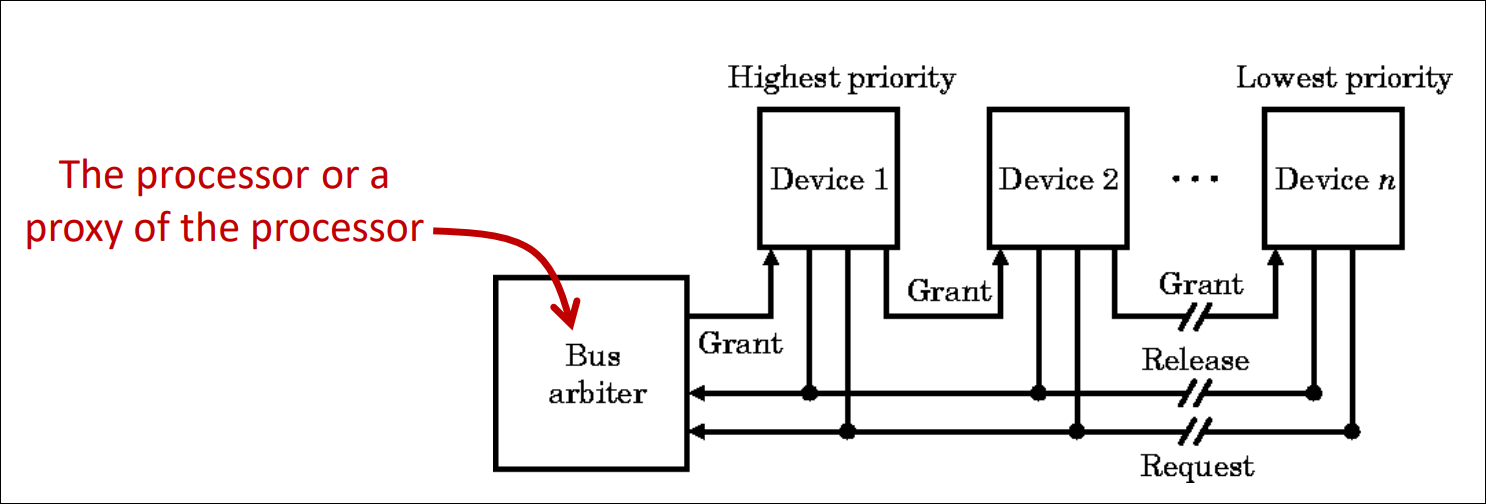
\includegraphics[scale=0.2]{screenshots/2025-10-22_15.png}
	\end{center}
\end{parag}

\subsection{Direct Memory Access (DMA)}

Even when using interrupts, the processor can spend a significant amount of time transferring data to and from input/output devices. This is especially problematic when dealing with high-throughput peripherals such as disks or network interfaces, where large amounts of data need to be moved. To address this inefficiency, the concept of Direct Memory Access (DMA) is introduced. With DMA, a dedicated hardware peripheral takes over the task of transferring data between memory and the I/O devices. This allows the CPU to continue executing other instructions while the data transfer occurs in parallel. By offloading these memory operations to the DMA controller, overall system performance is improved, and the CPU is no longer tied up managing large data transfers.\\
This idea shortly is:
\begin{itemize}
	\item Let’s have a \important{special peripheral} perform the needed data transfers from and to memory (R/W) and free the processor to continue computation
\end{itemize}
\begin{parag}{Without DMA}
    What we used to do before is:
	\begin{enumerate}
	    \item The peripheral launch a interrupt request
	    \item The Processor load the data from the peripheral
	    \item The processor store the data into the memory
	\end{enumerate}
	This processor can be done for like 1,000,00 times.
\end{parag}
\begin{parag}{With the DMA}
    The idea now is to:
	\begin{enumerate}
	    \item The peripheral launch a interrupt request
	    \item The processor launch it back to the DMA (with the needed informations)
	    \item The DMA load 
	    \item The DMA store it to the memory
	\end{enumerate}
	We do the same thing as before except the \textit{boring} part of load store, load, store, load, store ... is done by the DMA.
	\begin{center}
	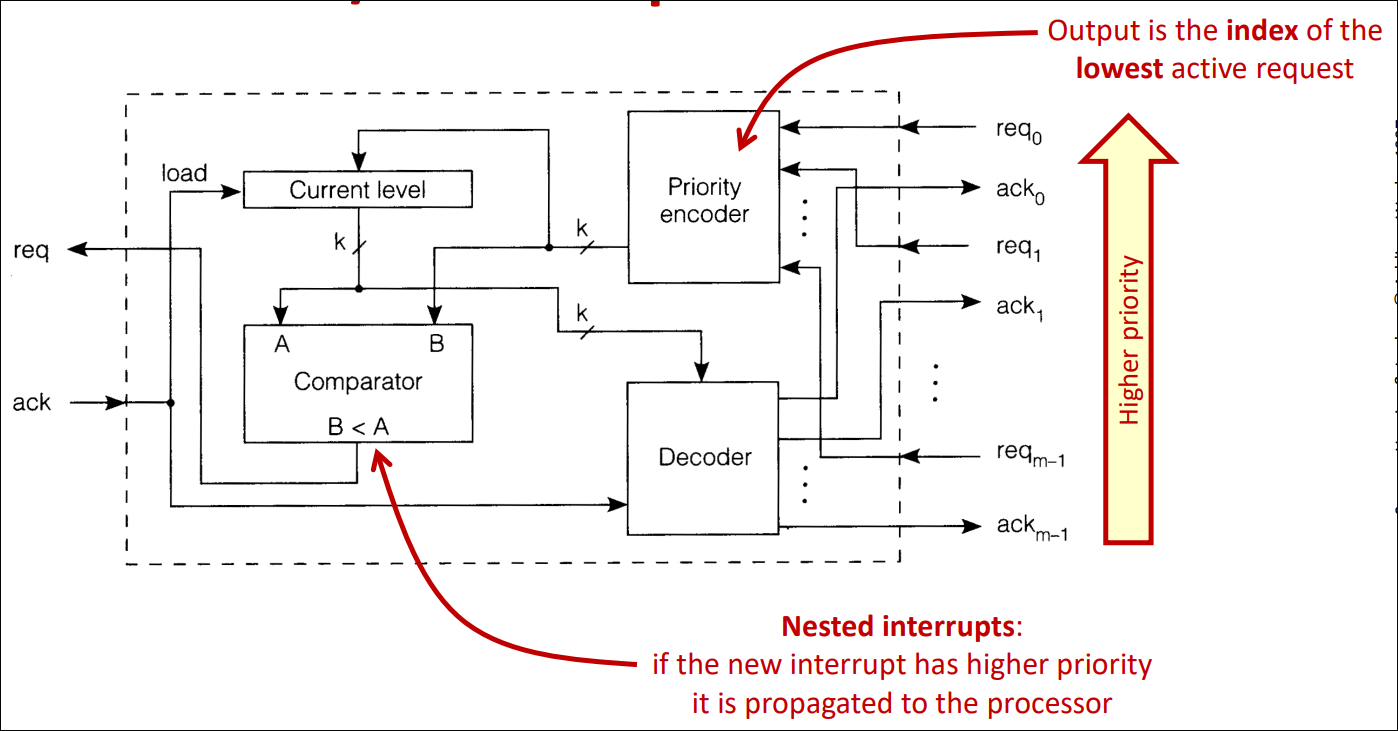
\includegraphics[scale=0.2]{screenshots/2025-10-22_16.png}
	\end{center}
	\begin{framedremark}
	I put only one screen here but there were like a nice way of introducing it in the slide so I'll just say it there, this is the 2.c. interrupts slide 14 to 24.
	\end{framedremark}
\end{parag}
\begin{parag}{Direct Memory Access}
   \begin{definition}
   A minimal DMA is:
   \begin{itemize}
       \item An \important{increment register} (how many bytes/words to transfer at a time)
       \item A couple of \important{address pointers} (source address pointer and destination address pointer), incremented by the above constant at every transfer 
       \item A \important{counter} (total number of bytes/words to transfer).
   \end{itemize}
   \end{definition} 
   \begin{subparag}{Example}
       Here an example of a sequence:
	   \begin{enumerate}
	       \item The processor tells the DMA controller (a) which device to access, (b) where to read or write the memory, and (c) the number of bytes to transer.
	       \item The DMA controller becomes bus master and performs the required accessses controlling directly the address and control busses.
	       \item The DMA controller sends an interrupt to the processor to signal succesful completion or erros
	   \end{enumerate}
	   
   \end{subparag}
\end{parag}



\begin{parag}{Timer and Periodic DMA Operations}
    In some cases, we want DMA transfers to happen at regular intervals without the CPU constantly supervising them. This is where a \important{timer} comes in. A timer is a hardware peripheral that counts up (or down) automatically and can generate an \important{interrupt} when it reaches a programmable maximum value. By configuring a timer, the CPU can schedule periodic DMA operations, such as reading data from a sensor every millisecond or streaming data from a peripheral continuously. This mechanism allows the DMA to start transfers on its own, triggered by the timer interrupt, freeing the CPU from constantly checking or initiating these operations.
\end{parag}

\begin{parag}{Bus Control and Processor Cooperation}
    During a DMA transfer, the DMA controller must temporarily take control of the memory bus, becoming the \important{bus master}. The processor must \important{relinquish control of the bus} during this period, but it can continue executing instructions that do not require bus access, such as computations using registers. Once the DMA completes the transfer, it sends an interrupt to the processor to signal successful completion or report any errors. This cooperation ensures that both CPU and DMA operate efficiently without conflicts on the memory bus.
\end{parag}

\begin{parag}{Advantages of DMA}
    Using DMA brings several benefits to a system:
    \begin{itemize}
        \item It offloads repetitive memory transfer tasks from the CPU, reducing workload.
        \item It increases system throughput, especially for large data blocks from high-speed peripherals.
        \item It allows the CPU to focus on computation or other tasks while data transfers happen in parallel.
        \item It reduces the time the CPU spends in \important{busy-waiting} loops checking for I/O readiness.
    \end{itemize}
\end{parag}

\begin{parag}{Example Sequence with Timer and DMA}
    An example sequence of operations with a timer and DMA could be:
    \begin{enumerate}
        \item The timer reaches its programmed max value and generates an interrupt.
        \item The processor acknowledges the timer interrupt and instructs the DMA controller to start a transfer from a peripheral to memory.
        \item The DMA controller becomes the bus master and performs the required memory accesses, reading from the peripheral and storing into memory.
        \item Once the transfer is complete, the DMA sends an interrupt to the processor to indicate completion.
        \item The CPU resumes normal execution, potentially until the next timer-triggered DMA transfer.
    \end{enumerate}
    This sequence illustrates how CPU, DMA, timer, and peripherals interact to efficiently handle high-throughput data transfers.
\end{parag}







\lecture{10}{2025-10-11}{Processor and converter}{}
\section{Exceptions}
We we still need to do one thing which is more in the hardware side: how can we handle running multiple programs at the same time? The goal is to \textit{fool} the user into believing that the programs are running at the same time.\\
The idea on how to do that is to execute each program in small delta time, we run a program for 10ms then we stored all the value of the register somewhere, run the other program for 10 ms, store the registers value, restore the first registers values etc.\\
Another issue is also privacy on computer with multiple users, a user should not be able to go the packet that was coming because maybe this packet was for another user. What we need here is a \textit{superuser} (which will be the os) that can check at who the packet is and wether or not gives it. We need to forbid some users to do a I/Os access
\begin{center}
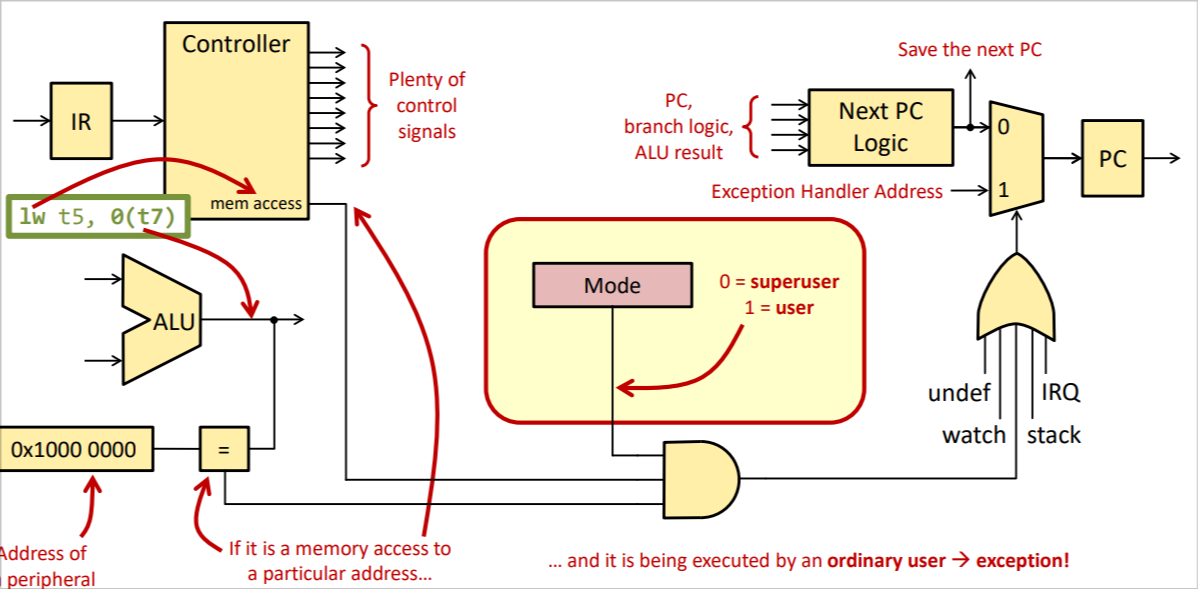
\includegraphics[scale=0.3]{screenshots/2025-10-15.png}
\end{center}
We check is the value is a memory access and it is at the place that I care $\implies$ I launch an exception. The \texttt{Mode} register is the information which allows us to know if we are the superuser or not, the implementation is \important{trivial}: adding an input at the and gate. We \important{need} two Mode otherwise we are cooked, Some questions that I found intresting during the lecture was: "\textit{isn't juste hardcode in the hardware? Why do we have only one Mode not like three or four?}".\\
But here we need an instruction to change from a mode to another, we need to be able to go    
\begin{align*} \text{user} \longleftrightarrow \text{superuser}   \end{align*}
However this is dangerous, imagine being a user being able to go to superuser and using the code of the user, when changing of user mode, we will also have to change the code that we are currenlty running.\\
But here using an exception is just a \textit{cosmetic} way of doing it, this is not an exception as the the pure sens of it.
\begin{parag}{Levels of Priviledge = Processors modes}%
\begin{itemize}
    \item Distingush \important{at least} two Processor \important{mode} :
		\begin{itemize}
		    \item \important{user mode} for the user's programs 
		    \item \important{Kernet, Supervisor, Executive}, etf for the os (kernel)
		    \item RISC-V has up to three: Machine, Supervisor, User
		\end{itemize}
		\item Have a part of the \important{processor state readable by all}, but only \important{writable with highest levels or priviledge}; at least a ;
			\begin{itemize}
			    \item Current \important{mode register}
			    \item Other configuration register (we will see some when discussing the memory hierarchy)
			\end{itemize}
			\item Method to \important{switch mode} back and forth
				\begin{itemize}
					\item A \important{dedicated instruction} to trigger a \important{software exception} and an instruction to \important{reset}
					\item RISC-V has ecal (system call) and mret sret (return from exception).
				\end{itemize}
\end{itemize}
\end{parag}
\subsubsection{Processor tasks on Exceptions}
What the processor should or could do when an exception is raised (depending on processors and type of exceptions):
\begin{itemize}
    \item Mask further interrupts 
    \item Save EPC
    \item Save information on the reason for the exception
    \item Modify privilege level (exception handler srun in some privileged mdoe)
    \item Free up some registers (e.g., copying them to shadow registers, where supported)
    \item Jump to the handler
\end{itemize}
Most or all these tasks are \important{reverted implicitly} with special instructions on exit
\begin{itemize}[noitemsep]
	\item \texttt{mret} in RISC-V reverts the privilege level and the interrupt enable
\end{itemize}
Some have to be \important{reverted explicitly by the handler}
\begin{itemize}
    \item Programmers may want to unmask further interrupts \important{as soon as it is safe}
\end{itemize}
\begin{parag}{Priorities}%
\label{par:Priorities}
We have seen that hardware \important{interrupt controllers} can help managing priotities (which interrupts is more urgent to serve?). Yet, this only affects the order IRQs are presented to the processor. But we may also want to \important{serve a high-priority interrupt while serving a lower priority one}\\
Alas, there is only one \texttt{mepc} and \texttt{mcause} register, and this is why, as soon as the processor takes an interrupt, it \important{must disable further interrupts}... What can we do?\\
\begin{itemize}
    \item Save critical information about the interrupt (\texttt{mepc, mcause, mstatus}) on some \important{same stack}, so that CSRs can be overwritten by further interrupts.
    \item Manually \important{reenable interrupts} (\texttt{mstatus}) without returning from the handler
\end{itemize}
\begin{framedremark}
The idea behind this is the same as the one when calling function and memory, we first though of having a \textbf{static} memory like here. however this won't works with recursive function for instance. What we do instead is to dynimcally allocate memory space in the stack. This is the same principle here.
\end{framedremark}
\end{parag}
\begin{parag}{Writing the handlers is very \important{very} tricky}%
\label{par:Writing the handlers is very \important{very} tricky}
Writing exception  handler is a \important{difficult task}!
\begin{itemize}
    \item Maybe the \important{stack cannot be used} (e.g., the exception results from a stack overflow)
    \item Maybe the \important{exception handler cannot be interrupted} (e.g., the handler uses static locations to save data including \texttt{mscratch}) and is therefore a nonreentrannt procedure)
    \item Maybe the \important{system cannot withstand not serving interrups} for a long time (e.g., I/Os buffers fill up)
\end{itemize}
Buggy \important{device drivers} from venders of peripherals (invoked by the interrupt handler of the operating system and running in some privileged mode) are often responsible for operating system instability.\\
\begin{framedremark}
This is why microsoft \important{formally verifies} and \important{certifies} device drivers.
\end{framedremark}
\end{parag}
\begin{parag}{Processor design Issue with Exceptions}%
\label{par:Processor design Issue with Exceptions}
Handling excpetions is \important{one of the biggest challenges} of high-performance processor design\\ Great difficulties in determining the exact state of execution and supporting a \important{precise restart mechanism}\\ 
Older processors did not support at all precise exceptions -- \important{Every exception was a terminations one,} and thus things were easy. We will seel this more in detail later in CS-200 and in eletive courses.\\
Now let us go back from what we have seen last week.
We debated if we could do something better, at the moment, to have access to the data, we were deciding when to read the data with the signal (DTACK) 

\begin{center}
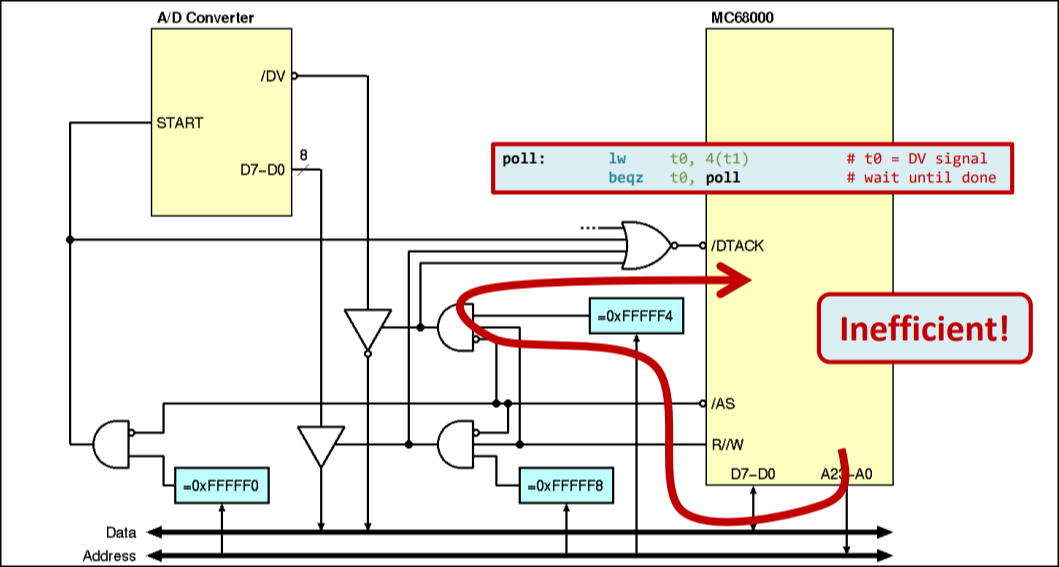
\includegraphics[scale=0.3]{screenshots/2025-10-17.png}
\end{center}
However this is pretty ineficient, the processor has to always check weither the signal is active or not instead of doing real work.\\
The goal here is to improve the interface to the A/D converter so that:
\begin{itemize}
    \item Any access (R or W) to address \texttt{oxFFFFF0} starts a new conversation 
    \item Upon completion, the A/D converter raises an interrup through the appropriate interrupt request signal of the proccessor.
    \item The result of the conversion can be ready by the processor at address\texttt{oxFFFFF8}
\end{itemize}
Suppose that our 8-bite preoccessor has an internal interrupt controller with various \texttt{IREQ}/\texttt{IACK} signap pairs for I/O interrupt requets\\
We have been assigned for our ADC these:
\begin{itemize}
    \item \texttt{IREQ3}: input,, dedicated to our peripheral to request attention
    \item \texttt{IACK3} output; used by the processor to signal to our peripheral that the request is acknowledged and is being served
\end{itemize}
\begin{center}
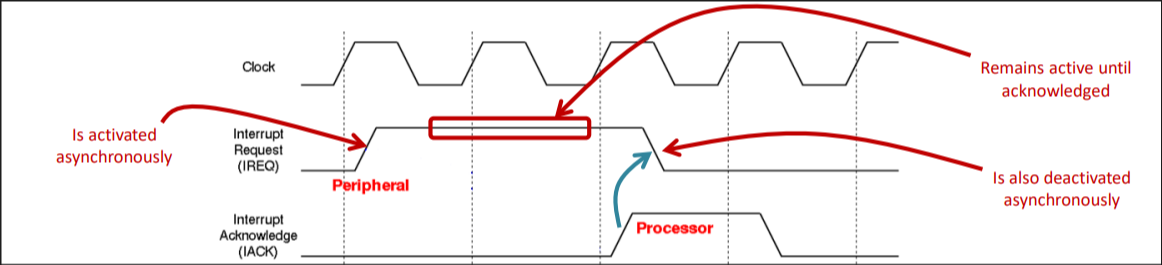
\includegraphics[scale=0.3]{screenshots/2025-10-17_1.png}
\end{center}
There is two main things here to acknowledged:\\
First, what we can see is that between the IREQ and the processor responds, we don't have a clock edge, this means that the acknowledged is only combination logic here.\\
On the other hand, we also see here that the IREQ here stays up until it is acknowledged, this means that we need to store the "up state"  for more than one clock cycle. What does this means? $\implies $ \important{flip flop}, we will ne a flip flop that store this information for us. What is weird about this flip flop is that the input that is store in it is 1, not the input value. The one deciding when it goes up or not is the A/D converter. This is looking very ugly\ldots 
\begin{center}
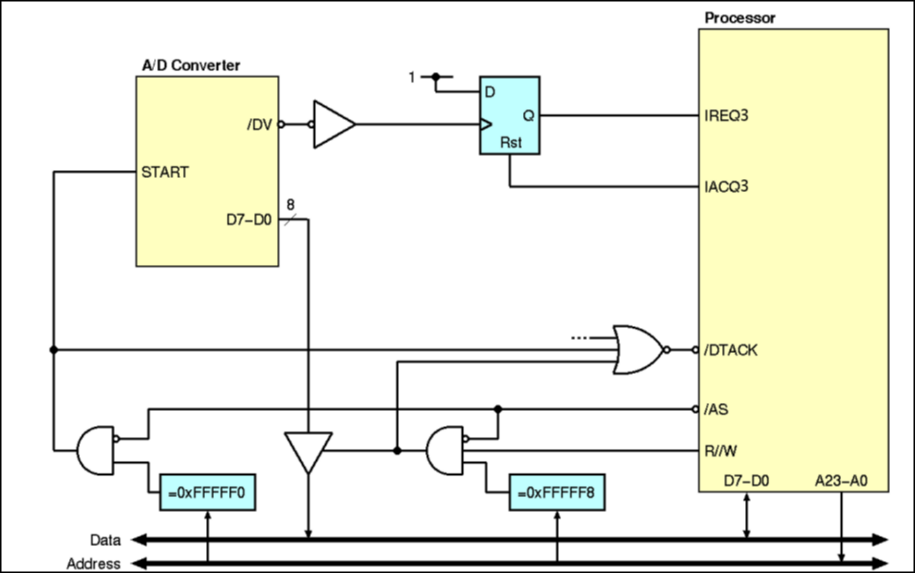
\includegraphics[scale=0.3]{screenshots/2025-10-17_2.png}
\end{center}
But why is this an error in any other context forbidden?\\
$\implies $ any flip flop \important{must} be connected to the clock of the system.

\end{parag}

\begin{parag}{A/D converter: startADC}
	this is a pretty trivial task to do
	\begin{lstlisting}[language={[RISC-V]Assembler}]
	startADC:	lui t0, 0xfff
				addi t0, t0, 0xff0 # to = 0xfffff0
				sw zero, 0(t0)

				ret
	\end{lstlisting}
\end{parag}
\begin{parag}{Handler}
    On the other hand the handler part is a bit harder.\\
	For instance the handler:\\
	
	\begin{lstlisting}[language={[RISC-V]Assembler}]
startADC:	addi sp, sp, --
			..
			..
			csrr t0, mcause

			..
			jal readADC
			jal buffer #we need to store the information somewhere for other to have access to it
			..
			mret
	
	\end{lstlisting}
	\begin{framedremark}
	The \texttt{mcause} is the register which stores the machine external interrupt
	\end{framedremark}
	So the real part for this is:
	\begin{lstlisting}[language={[RISC-V]Assembler}]
handler:	addi sp, sp, -120 # save all registers but zero and sp
			sw x1, 0(sp)
			sw x3, 4(sp)
			.. etc ..
			sw x31, 116(sp)

			csrr s0, mcause # Read exception cause
			bgez so, handleException #branche if not an interrupt (MSB = 0, looks like zero or a positive number..)
			slli s0, s0, 1 # Get rid ofthe MSB of s0, so that what is left is the cause
			srli s0, s0, 1 
			li s1, 11 
			bne s1, s2, handleOtherInts # Branch if not an external interrupt

			jal readADC  # return a0 = ADC result 
			jal insertIntoBuffer  # Gets a0 = value to add to a circular buffer

restore:	lw x1, 0(sp)
			lw x3, 4(sp)
			.. etc ..
			lw x31, 116(sp)

			addi sp, sp, 120
			mret
	\end{lstlisting}
	
\end{parag}
\begin{parag}{A/D converter: insertIntoBuffer}
	\begin{lstlisting}[language={[RISC-V]Assembler}]
.section .data 	
		.equ bufferSize, 1024 #define buffer size 
		.equ bufferBytes, bufferSize * 4 # compute the total size in bytes for the buffer 

bufferPointer: 	.word 0  # Initializse the pointer index to 02d
buffer: 		.space bufferBytes  # Allocate space for bufferSize * wordsize bytes

.section .text 
insertIntoBuffer: 	
	la t0, la t0 bufferPointer # Load address of budderPointer into t0
	lw t1, 0(t0) # Load current buffer pointer into t1
	la t2, buffer  # Load base address of the buffer into t2
	slli t3, t1, 2  # Multiply
	add t4, t2, t3 
	sw a0, 0(t4)
	addi t1, t1, 1 
	li t5, bufferSize - 1 
	and t1, t1, t5 
	sw t1, 0(t0)

	ret
\end{lstlisting}
\end{parag}









\lecture{12}{2025-10-17}{Example of I/O/s and Exceptions}{}
Today's lecture is an example of what we did the previous weeks.
\begin{parag}{Parti 1a: Connecting an Input Peripheral}
	Consider an hypothetical processor with the following buses and control signals
	\begin{itemize}
		\item \texttt{A[31:1]} $\to $ Address bus 
		\item \texttt{D[31:1]} $\to $ Data bus 
		\item \texttt{AS} $\to $ Address Strobe (active when a valide address is present on \texttt{A[31:0]})
		\item \texttt{WR} $\to$ Write (active with an ASS when performing a write cycle)
	\end{itemize}
	\begin{subparag}{Bus protocol}
	\begin{center}
	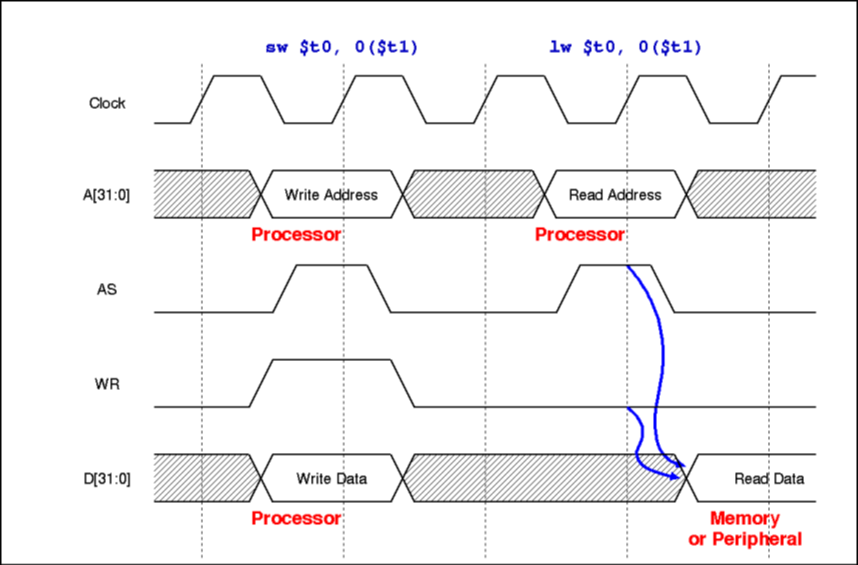
\includegraphics[scale=0.3]{screenshots/2025-10-17_3.png}
	\end{center}
    Here this is something that is very useful for us to read
	\end{subparag}
	\begin{subparag}{What do we want?}
	    \begin{itemize}
			\item Connect to the processor \important{10 buttons numbered from 0 to 9}
			\item Each button outputs a logic '1' if presse '0' otherwise 
			\item The processor must read the \important{state of the buttons} with a read from memory location \texttt{0xFFFF'FFF0}: '0' indicates no button pressed '1' indecates a button pressed 
			\item The processor must read the \important{number of the button pressed} with a read from memory location \texttt{0xFFFF'FFF4}.
	    \end{itemize}
	\end{subparag}
	The question now is: what do we need to do?\\
\end{parag}
\begin{parag}{Circuit}
    The first thing we need to do is to OR all the button together (so that if at least one of the button is pressed, the result woudd be one). Then we need to know which button is pressed. To do so, we need to decoode the buttons outputs into a 4 bits number $\implies $ we add a $2^n$ decoder. \\

	\begin{framedremark}
For the rest of the course I think the video is better than this because I cannot really explain it well while "drawing". 
	\end{framedremark}
\end{parag}



\chapter{Memory Hierarchy}
\lecture{12}{2025-10-17}{}{}
What we want now is to go back to memory and spent quite a lot of time on this topic. What we will change here is that we will care about the performance of the memory we are building.

\section{Caches}
The question we have is what is the problem with memory:
\begin{center}
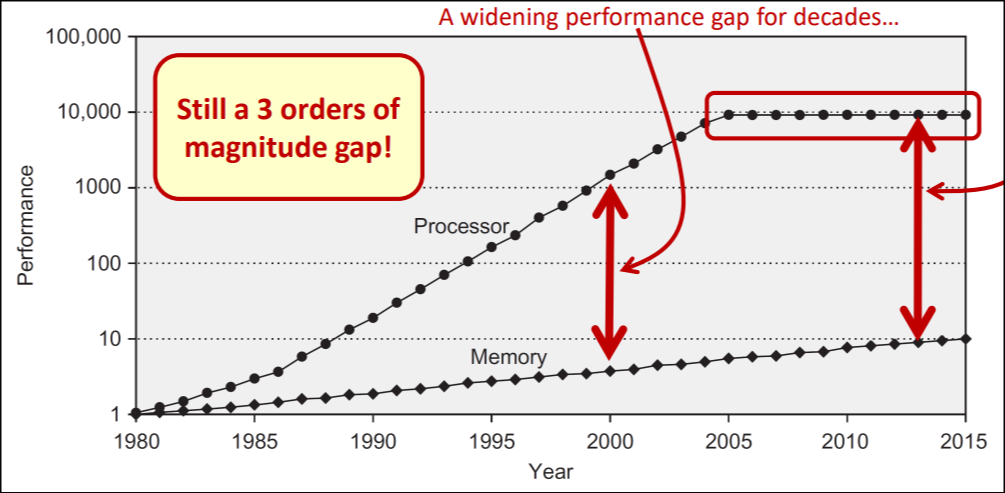
\includegraphics[scale=0.2]{screenshots/2025-10-17_6.png}
\end{center}
Processor has been improved a \important{lot} in comparisaison of memory. What memory means here is DRAM.\\
The issue is that we want a big memory and a fast processor which cannot really work well together, we need to \important{so something} ourself.\\
What we can do is to use other type of memory which is \important{faster but expensive} 
\begin{tikzpicture}[
    box/.style = {draw, minimum width=2.8cm, minimum height=1cm, align=center, font=\small},
    label/.style = {font=\footnotesize, align=center}
  ]

  % Processor node
  \node[box] (processor) {Processor};

  % Child nodes
  \node[box, below left=of processor, xshift=-1.5cm] (dram) {DRAM};
  \node[box, below=of processor] (sram1) {SRAM};
  \node[box, below right=of processor, xshift=1.5cm] (sram2) {SRAM};
  \node[box, below=of sram2, yshift=-0.8cm] (sram3) {SRAM};

  % Arrows from processor to memory
  \draw[->] (processor) -- (dram);
  \draw[->] (processor) -- (sram1);
  \draw[->] (processor) -- (sram2);
  \draw[->] (sram2) -- (sram3);

  % Annotations
  \node[label, below=0.1cm of dram] {30--50ns\\10--100GB};
  \node[label, below=0.1cm of sram1] {10--20ns\\1--10MB};
  \node[label, below=0.1cm of sram2] {3--10ns\\100KB};
  \node[label, below=0.1cm of sram3] {$<$1ns\\10KB};

\end{tikzpicture}


\begin{center}
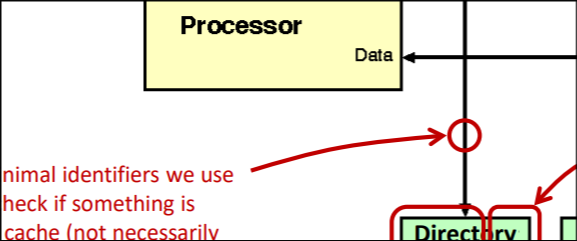
\includegraphics[scale=0.3]{screenshots/2025-10-17_7.png}
\end{center}


So the fact is: this is not only a technology issue even though we are not able to make \texttt{DRAM} faster. It's not even an issue with \texttt{SRAM} cost, it wouldn't be too costly to make \texttt{SRAM} bigger, the issue is that even though SRAM is pretty maleable, when expanding it, it becomes 2 to 3 degree of magnitude slower (in terms of clock cycles).

\begin{parag}{What memory to use?} The question is where do we put our data, in which memory.\\
	For instance let us took a look at this code:
	\begin{lstlisting}[langage=c]
i = 0;
sum = 0;
while (i < 1024) {
	sum = sum + a[i];
	i = i + 1; 
}
	\end{lstlisting}
	
	\begin{itemize}
	    \item Intruction corresponds to line 3-5 that are \important{read over and over}should be in fast memory
	    \item if variable \texttt{i} and \texttt{sum} are stored in memory, they are also \important{used often} and should be stored in fast memory
	    \item One would like to anticipate the future and load the \important{following} instructions and vector elements.
	\end{itemize}
\end{parag}
\begin{parag}{Spatial and Temporal locality}
    There is two important criteria for the choice of the placement:
	\begin{itemize}
	    \item \textbf{Temporal locality}
			\begin{itemize}
			    \item Data that have been \important{used recently}, have likelyhood of being used again (Code: loop, function, ...) (Data: local variables and data structures)
			\end{itemize}
			\item Spatial locality
				\begin{itemize}
				    \item Data which \important{follow in the memory other data} that are currently used are likelyhood to be used in the future (Code are usually sequential, Data: array)
				\end{itemize}
	\end{itemize}
	However, this is not perfect, this is onlyl a probablistic model. We are only making guess and hoping there were right so that we can win some time.
\end{parag}

\begin{parag}{Our placment policy most be:}
    \begin{subparag}{Invisible to the programmer}
        \begin{itemize}
            \item One could analyse data structures and program semantics to detect heabily used vairables/arrays and thus decide placment $\to$ OK in some context (emebedded) but we want to have the programmers not to go through this hassle 
            \item To do so, we will add \important{hardware} to help
        \end{itemize}
    \end{subparag}
	\begin{subparag}{Extremly simple and fast}
		The decision are made in the hardware, they need to be simple. The goal is to accesst memory very fast, in the order of a ns or less:  \important{not much time} to make a complex decision...
	\end{subparag}
\end{parag}


\subsubsection{Cache: The idea}
The main difference between this and the tree make before is that now as a \important{programmer} I don't know which memory I am using, I am at a level of abstraction above which makes it easier for me to develop software.\\
The idea behind the cache is the fololowing:\\
The processor makes a request for an address, we first check if the address is in the dirc





\end{document}
